% !TeX spellcheck = en_US
% !TeX encoding = UTF-8

\documentclass[aps, 10pt, a4paper]{article}

\usepackage{graphics, graphicx, graphics}
\usepackage{fancyvrb, enumerate}
\usepackage{amsmath, amssymb, amscd, amsfonts}
\usepackage{geometry}
\usepackage{multirow}
\usepackage{url}
\usepackage{tikz}
\usepackage{listings, listing}
\usepackage{color}
\usetikzlibrary{shapes, arrows, calc, positioning}

\definecolor{codegreen}{rgb}{0, 0.6, 0}
\definecolor{codegray}{rgb}{0.5, 0.5, 0.5}
\definecolor{codepurple}{rgb}{0.58, 0, 0.82}
\definecolor{backcolour}{rgb}{0.95, 0.95, 0.92}

\lstdefinestyle{mystyle}
{
    backgroundcolor=\color{backcolour},   
    commentstyle=\color{codegreen},
    keywordstyle=\color{magenta},
    numberstyle=\tiny\color{codegray},
    stringstyle=\color{codepurple},
    basicstyle=\footnotesize,
    breakatwhitespace=false,         
    breaklines=true,                 
    captionpos=b,                    
    keepspaces=true,                 
    numbers=left,                    
    numbersep=5pt,                  
    showspaces=false,                
    showstringspaces=false,
    showtabs=false,                  
    tabsize=2,
    frame=single
}
\lstset{style=mystyle}

\tikzstyle{decision} = [diamond, draw, fill=blue!20, text width=4.5em, text badly centered, node distance=3cm, inner sep=0pt]
\tikzstyle{block} = [rectangle, draw, fill=blue!20, text width=5em, text centered, rounded corners, minimum height=2em]
\tikzstyle{line} = [draw, -latex']
\tikzstyle{cloud} = [draw, ellipse, fill=red!20, node distance=5em, minimum height=2em]
\tikzset
{
    -|-/.style=
    {
        to path=
        {
            (\tikztostart) -| ($(\tikztostart)!#1!(\tikztotarget)$) |- (\tikztotarget)
            \tikztonodes
        }
    },
    -|-/.default=0.5,
    |-|/.style=
    {
        to path=
        {
            (\tikztostart) |- ($(\tikztostart)!#1!(\tikztotarget)$) -| (\tikztotarget)
            \tikztonodes
        }
    },
    |-|/.default=0.5,
}

\geometry
{
    top = 20mm,
    bottom = 20mm,
    left = 20mm,
    right = 20mm
}

\title{Lab Internship\\Summer 2019}
\author{Jaewoong Lee}
\date{\today}

\begin{document}
    \maketitle
    \newpage
    
    \tableofcontents
    \listoftables
    \listoffigures
    \newpage
    
    \section{Introduction}
        \subsection{Single Cell Analysis}
            In traditional, we have done RNA sequencing with bulk RNA input. With bulk RNA sequencing, we can know average gene expression from all cell, although, cellular heterogeneity is still veiled. 
            However, nowadays, we can analysis RNA sequencing with every single cell. Therefore, we investigate expression profile of each cell, then we reveal heterogeneity and sub-population expression variability of cells.
        
        \subsection{Principal Component Analysis}
            Principal component analysis (PCA) is a technique that finds an axis which preserves a variance of data, and then reduces high-dimensional data to low-dimensional. PCA is not a feature selection, which means choose the best feature amongst featues; but, it is a feature extraction, which means make new feature with subsist features.
        
        \subsection{T-Distributed Stochastic Neighbor Embedding}
            T-distributed stochastic neighbor embedding (TNSE) is a kind of machine learning technique, is used to dimensional reduction. Traditional dimensional reduction technique is hard to classify each manifolds in dimension reduced data. However, TSNE can preserve such manifolds in dimension reduced data with T-distribution. 
        
        \subsection{Clustering}
            Clustering is a algorithm which maximize inter-cluster variance and minimize inner-cluster variance. It is an unsupervised learning, not a classification, which means gathering each data for some group.
    
    \section{Method}
        \subsection{Cell Ranger}
            Cell Ranger is a set of analysis pipelines that process Chromium single-cell RNA-seq output to align reads, generate feature-barcode matrices and perform clustering and gene expression analysis. \cite{ref:cellranger}
        
        \subsection{Scikit-Learn}
            Scikit-Learn is a Python module for machine learning built on top of SciPy. \cite{ref:scikit}
    
    \section{Result}
        \subsection{Highly Variable Gene}
            At first, I chose highly variable gene amongst genes. Highly variable gene means genes have higher means and higher CV, where CV is defined as equation \ref{eq:cv}.
            \begin{equation}
                \rm{CV} = \frac{\rm{Variances}}{\rm{Means}}
                \label{eq:cv}
            \end{equation}
            
            The distributed map of whole gene is in a figure \ref{fig:hvg}. I chose 822 genes which is top 5\% of both means and CVs. 
            \begin{figure}[tbph]
                \centering
                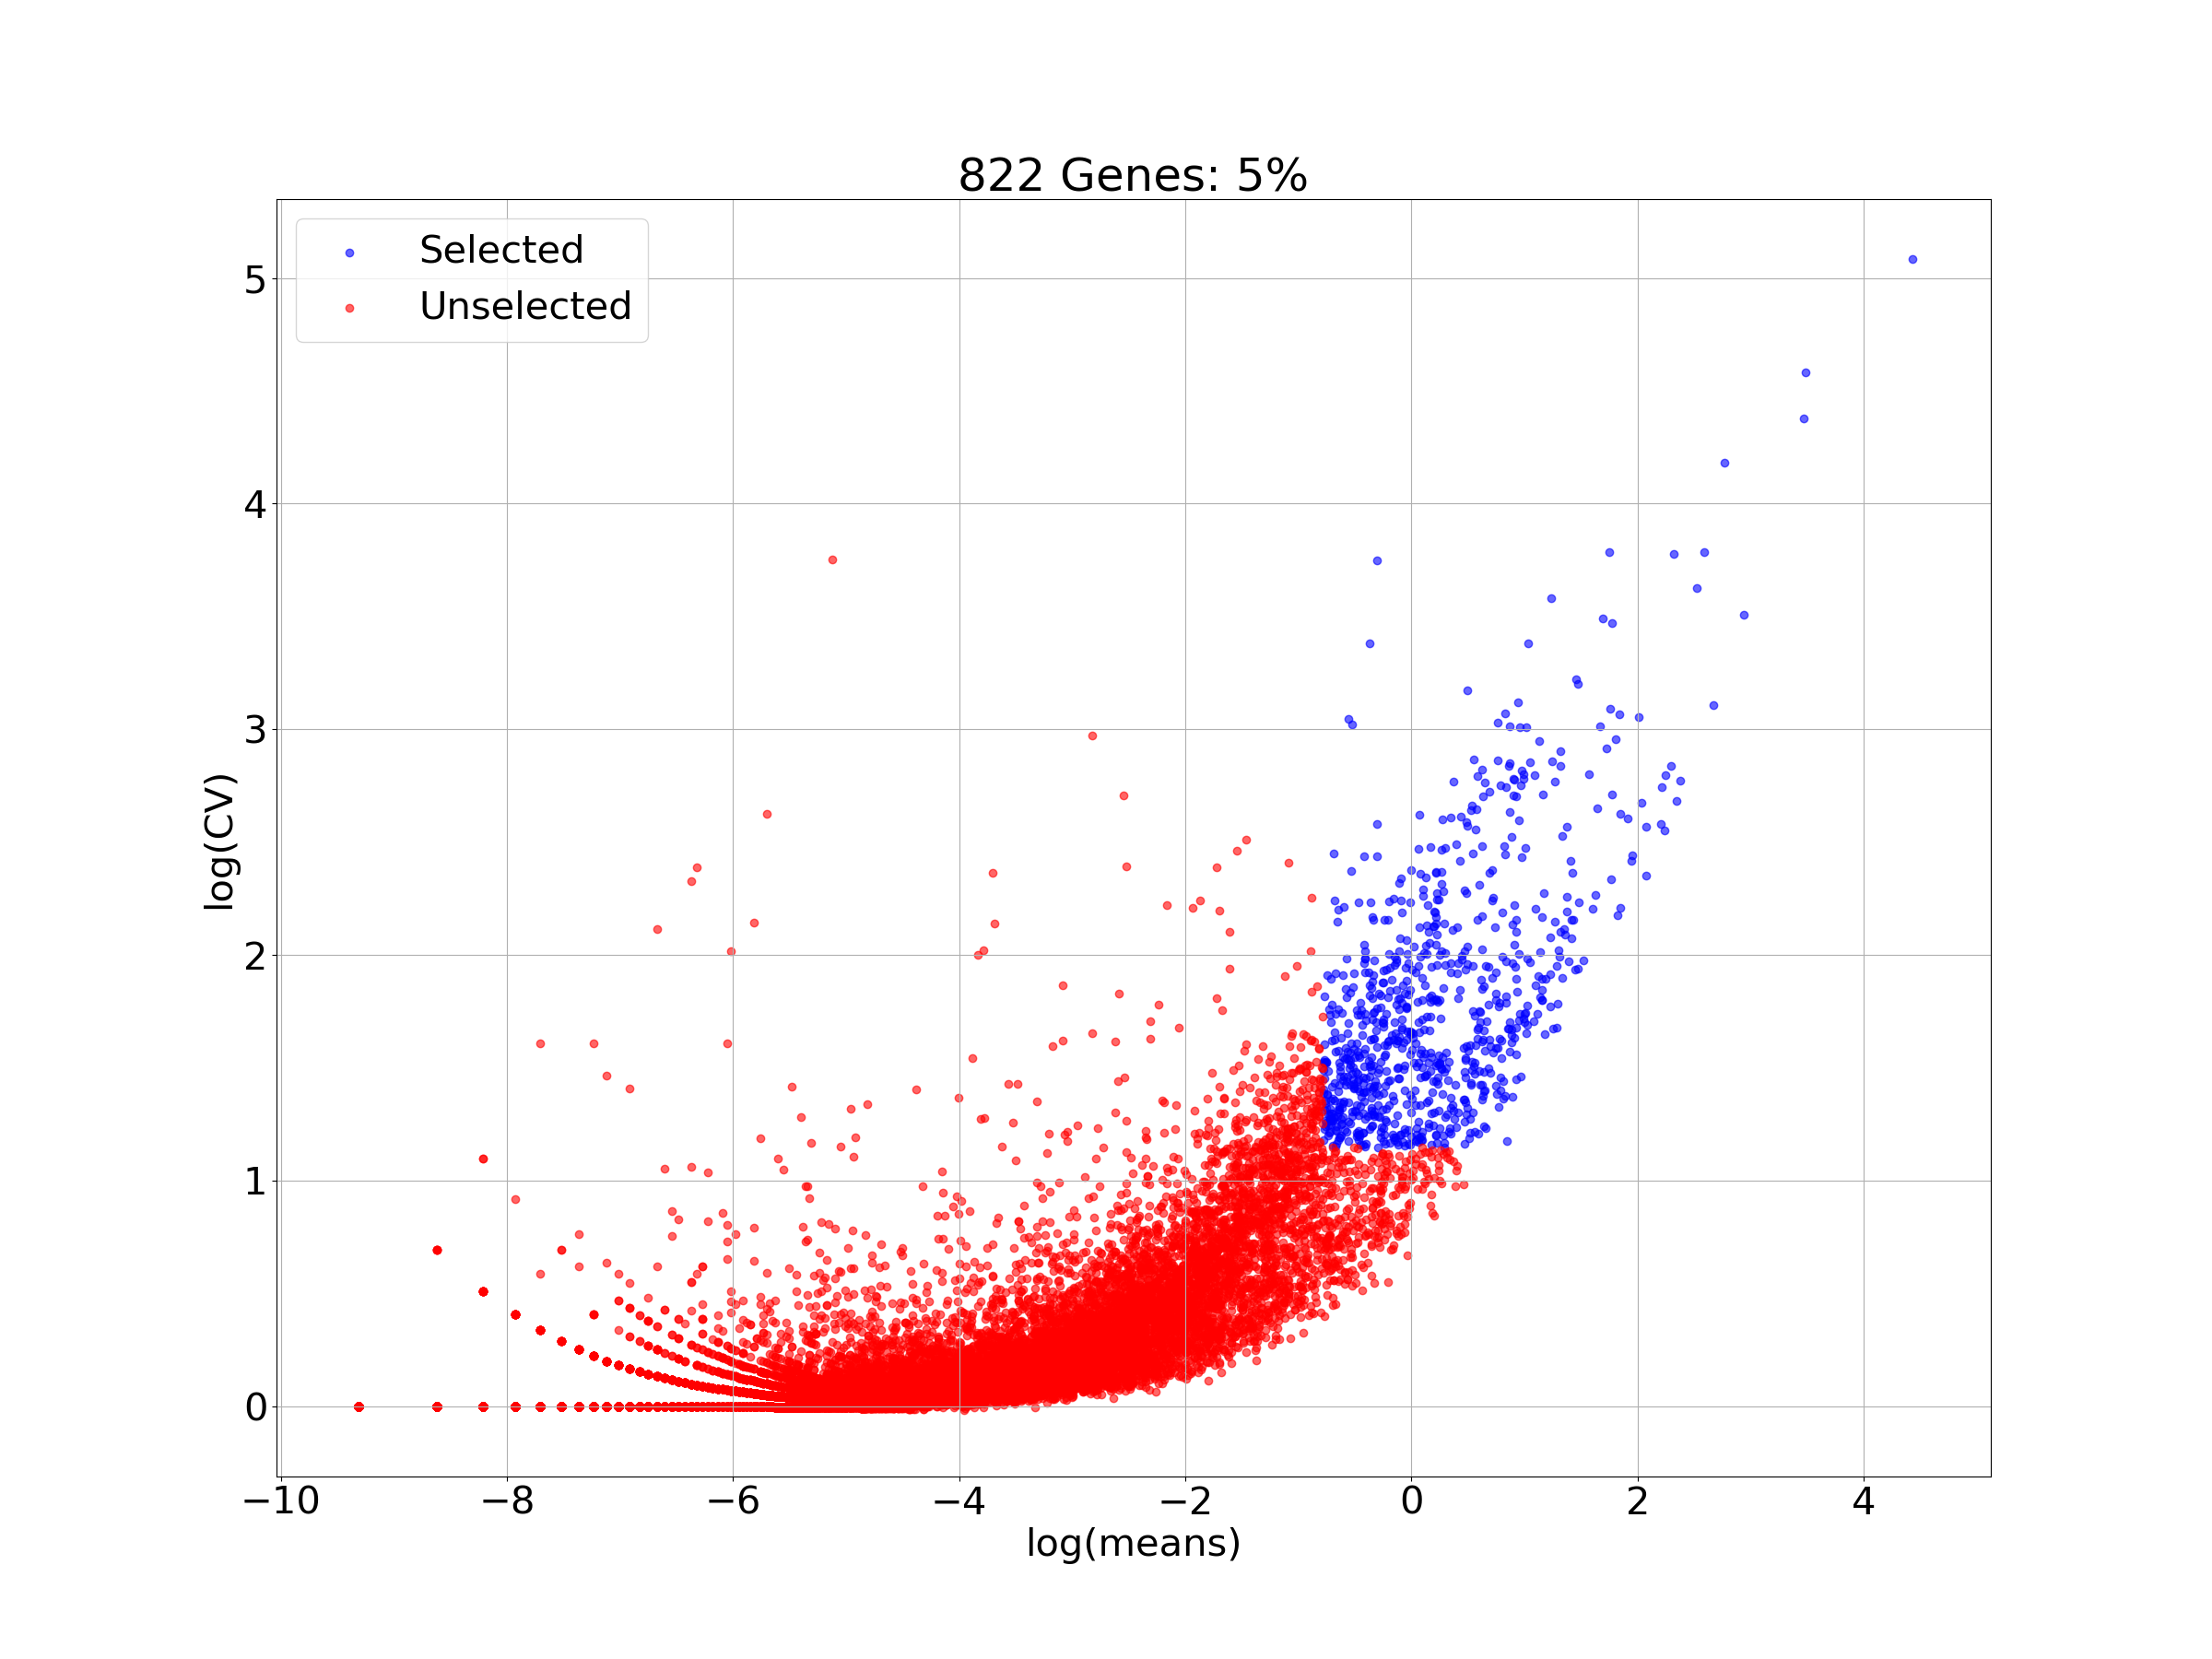
\includegraphics[height=8cm]{figures/HVG.png}
                \caption{Scatter Map of Whole Gene with Means vs. CVs}
                \label{fig:hvg}
            \end{figure}
        
        \subsection{PCA}
            With PCA, I reduced a matrix of cell by gene. For example, an original data is 11082 $\times$ 822 of cell by gene, but, with PCA, I reduced to 11082 $\times$ 792 of cell by gene-like. 
    
        \subsection{TSNE Map}
            The 2D TSNE map of each sample is in figure \ref{fig:2dtsne}.
            \begin{figure}[bph]
                \begin{center}
                    $\begin{array}{cc}
                        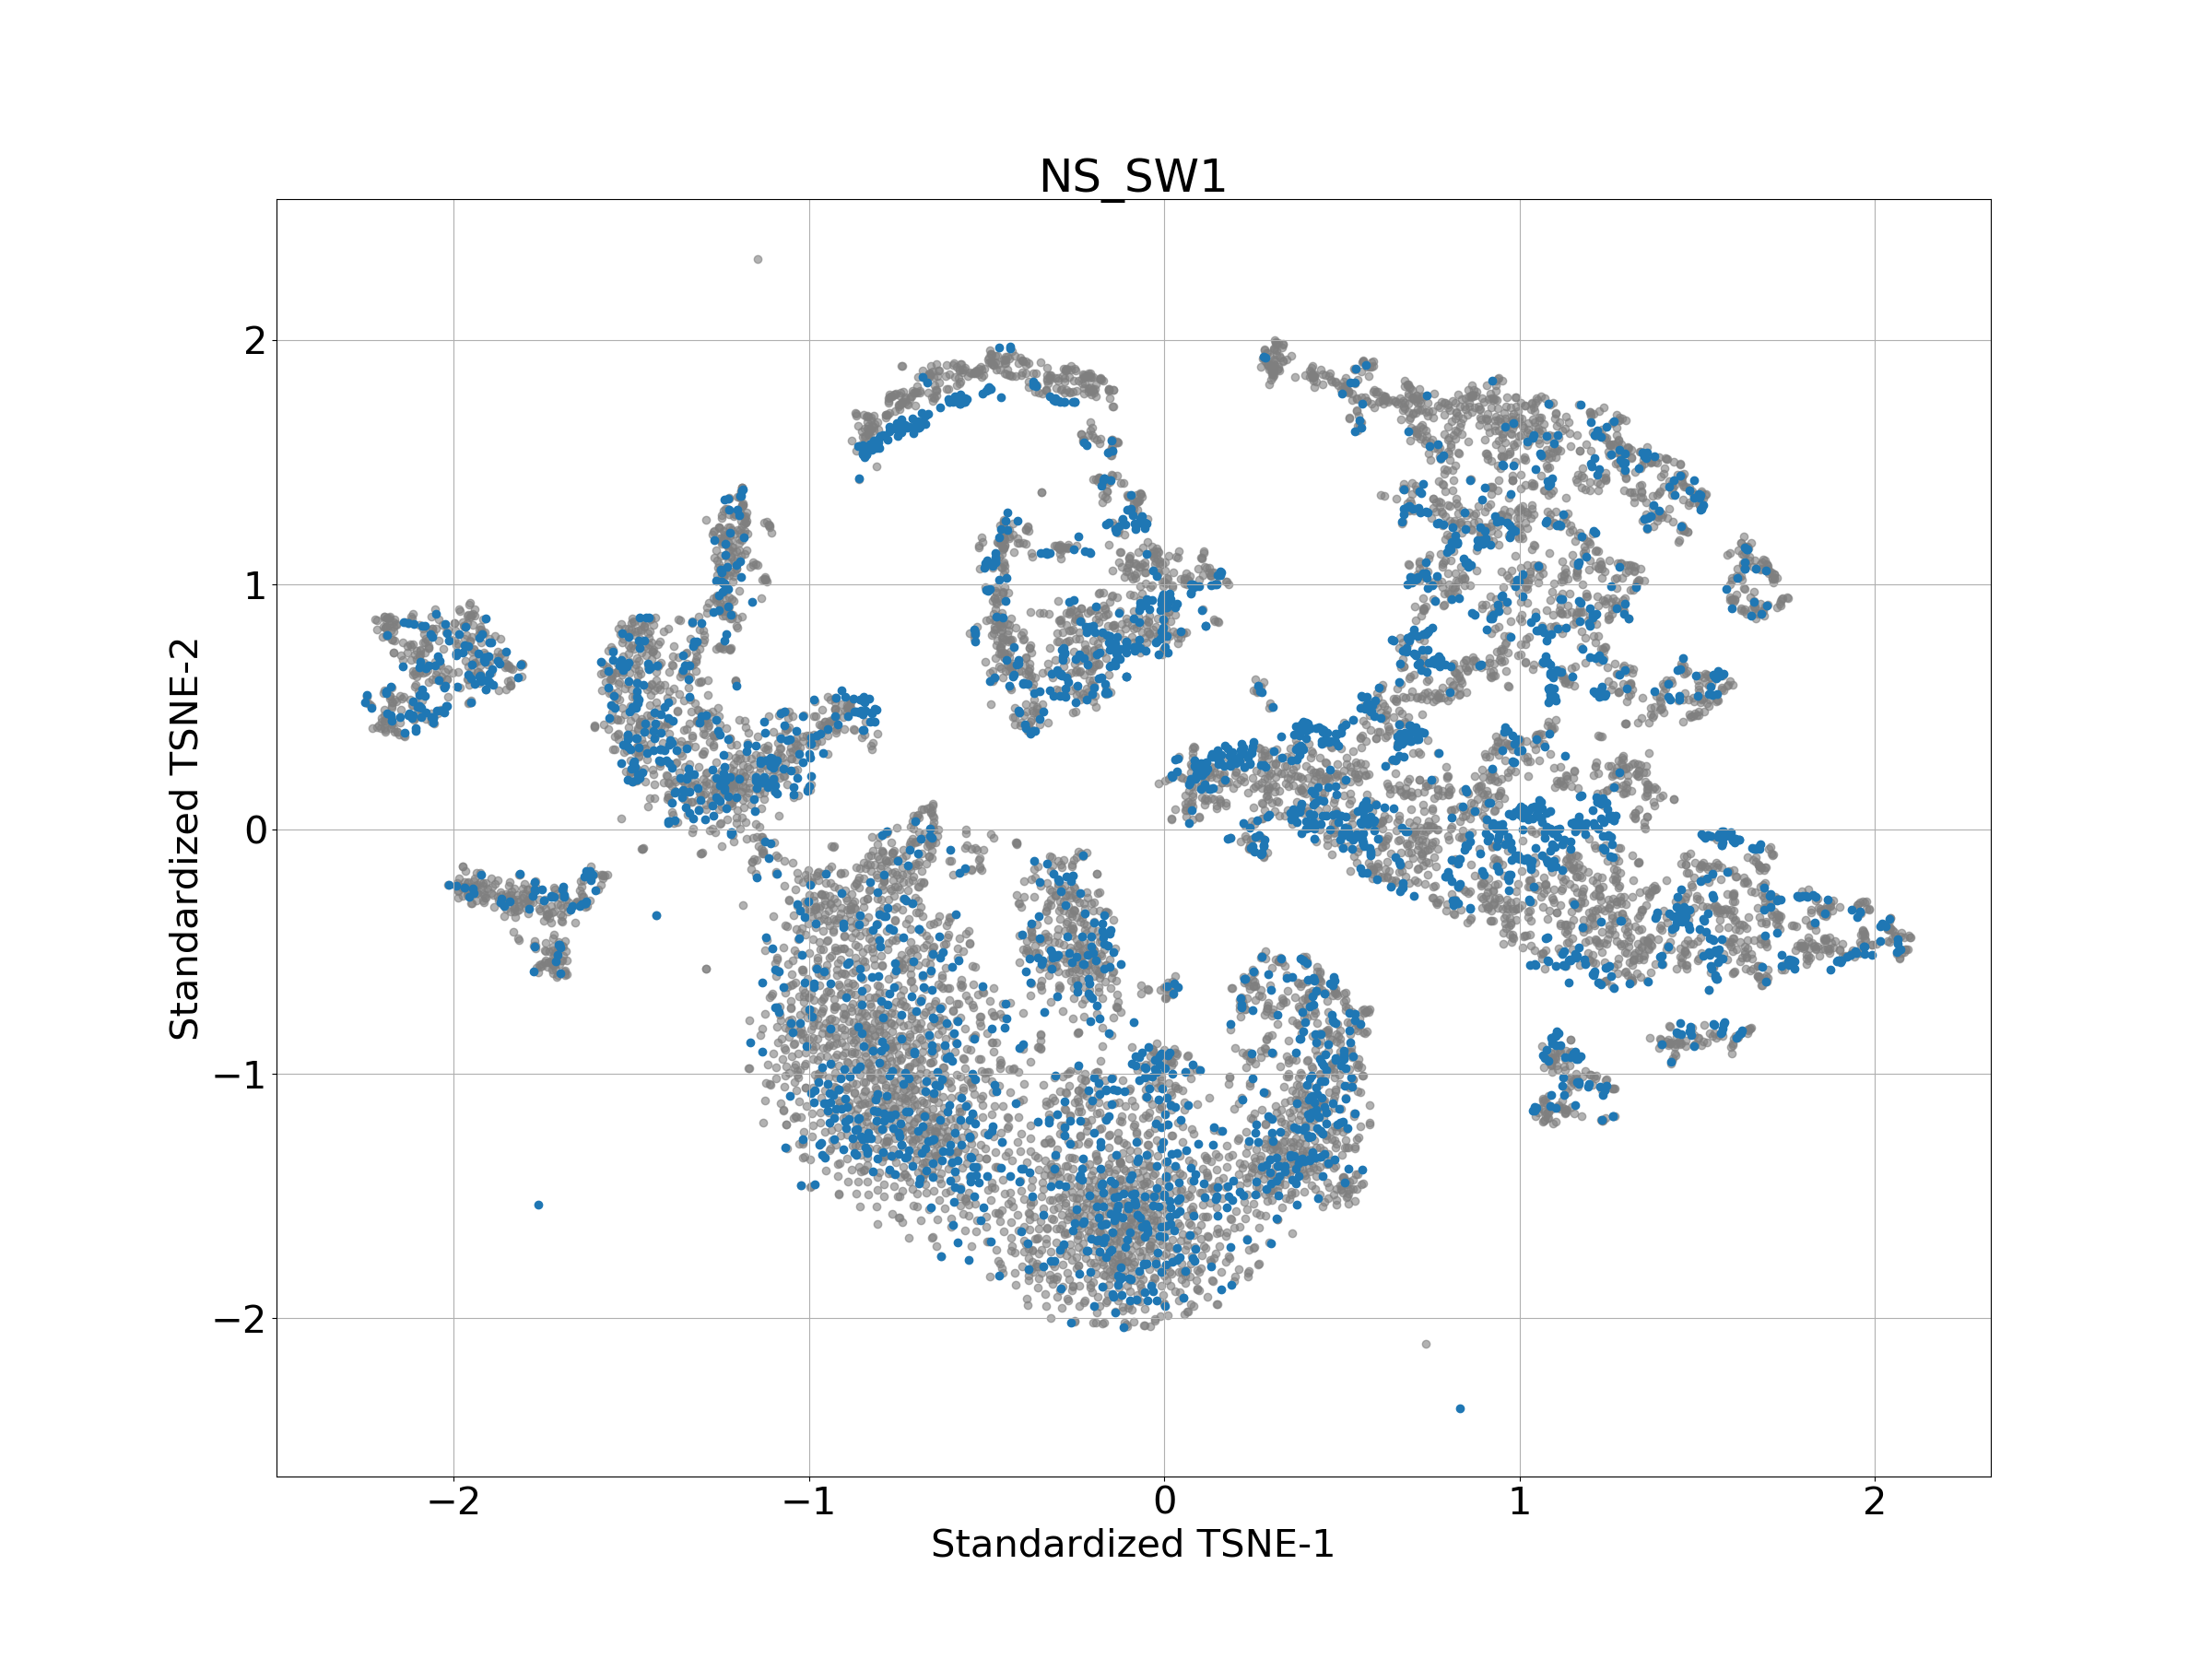
\includegraphics[height=5cm]{figures/TSNE/1.png}
                        &
                        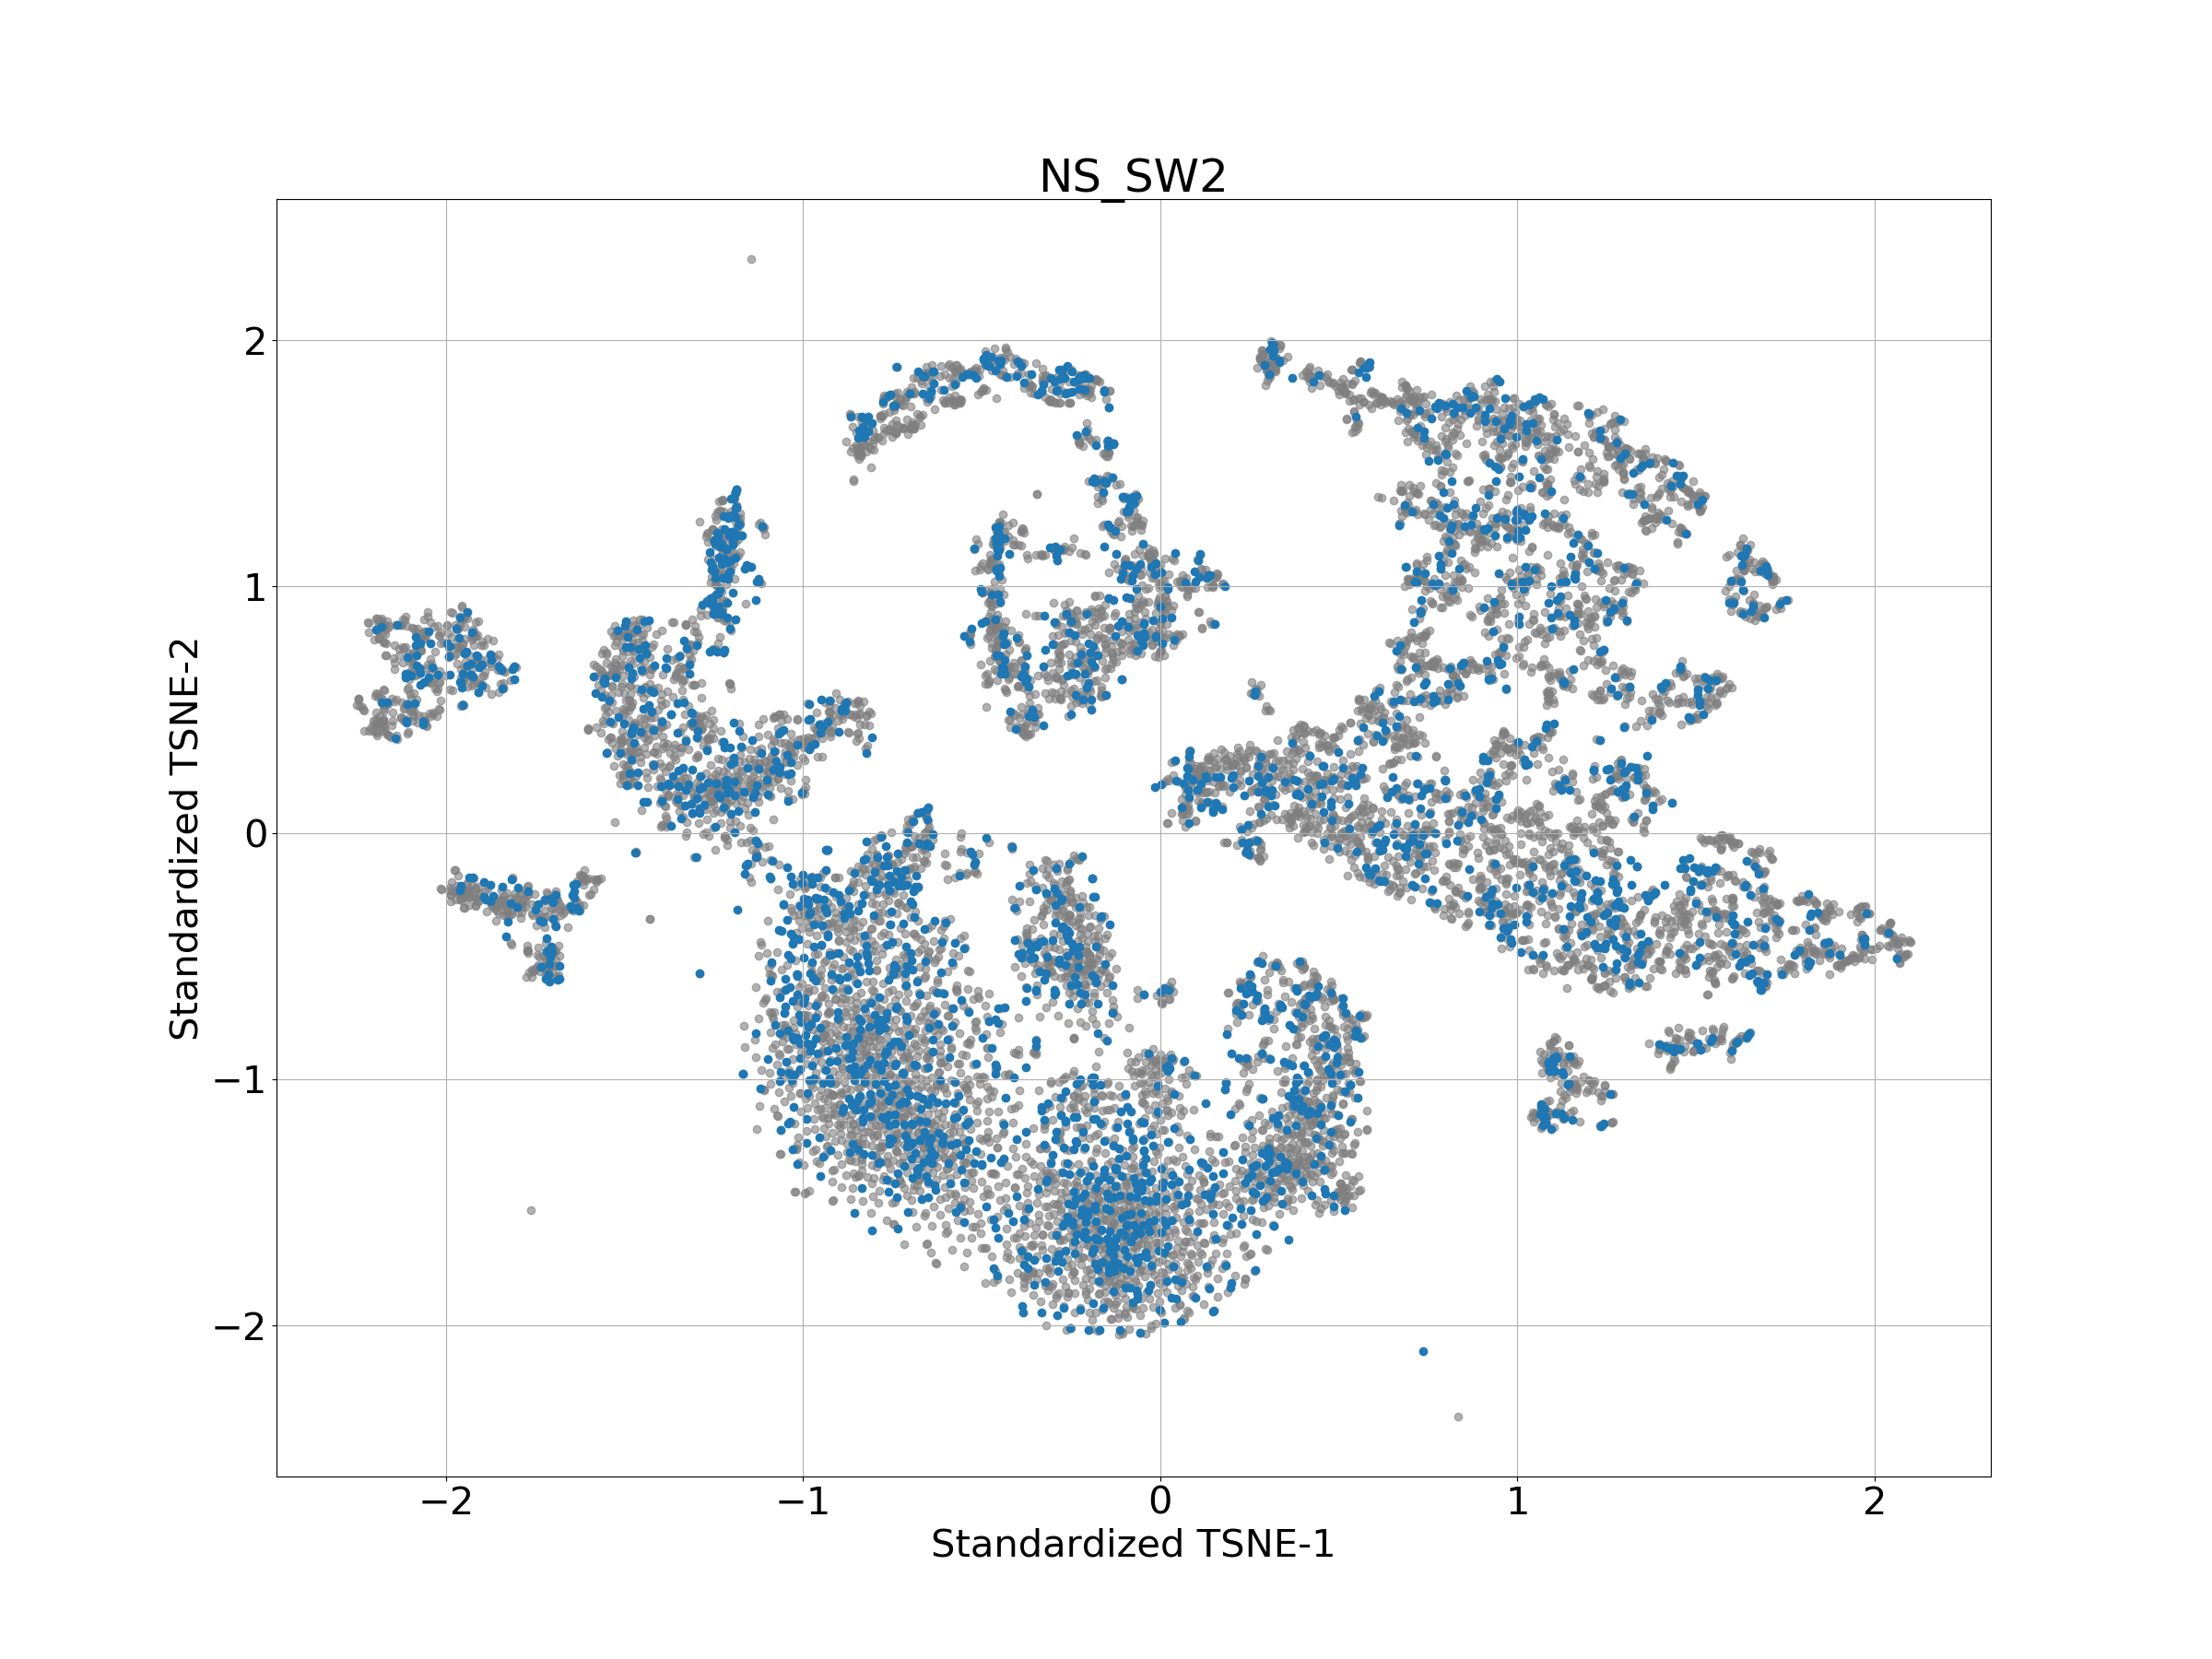
\includegraphics[height=5cm]{figures/TSNE/2.png}
                        \\
                        
                        \mbox{(a) NS\_SW1} & \mbox{(b) NS\_SW2} \\
                       
                       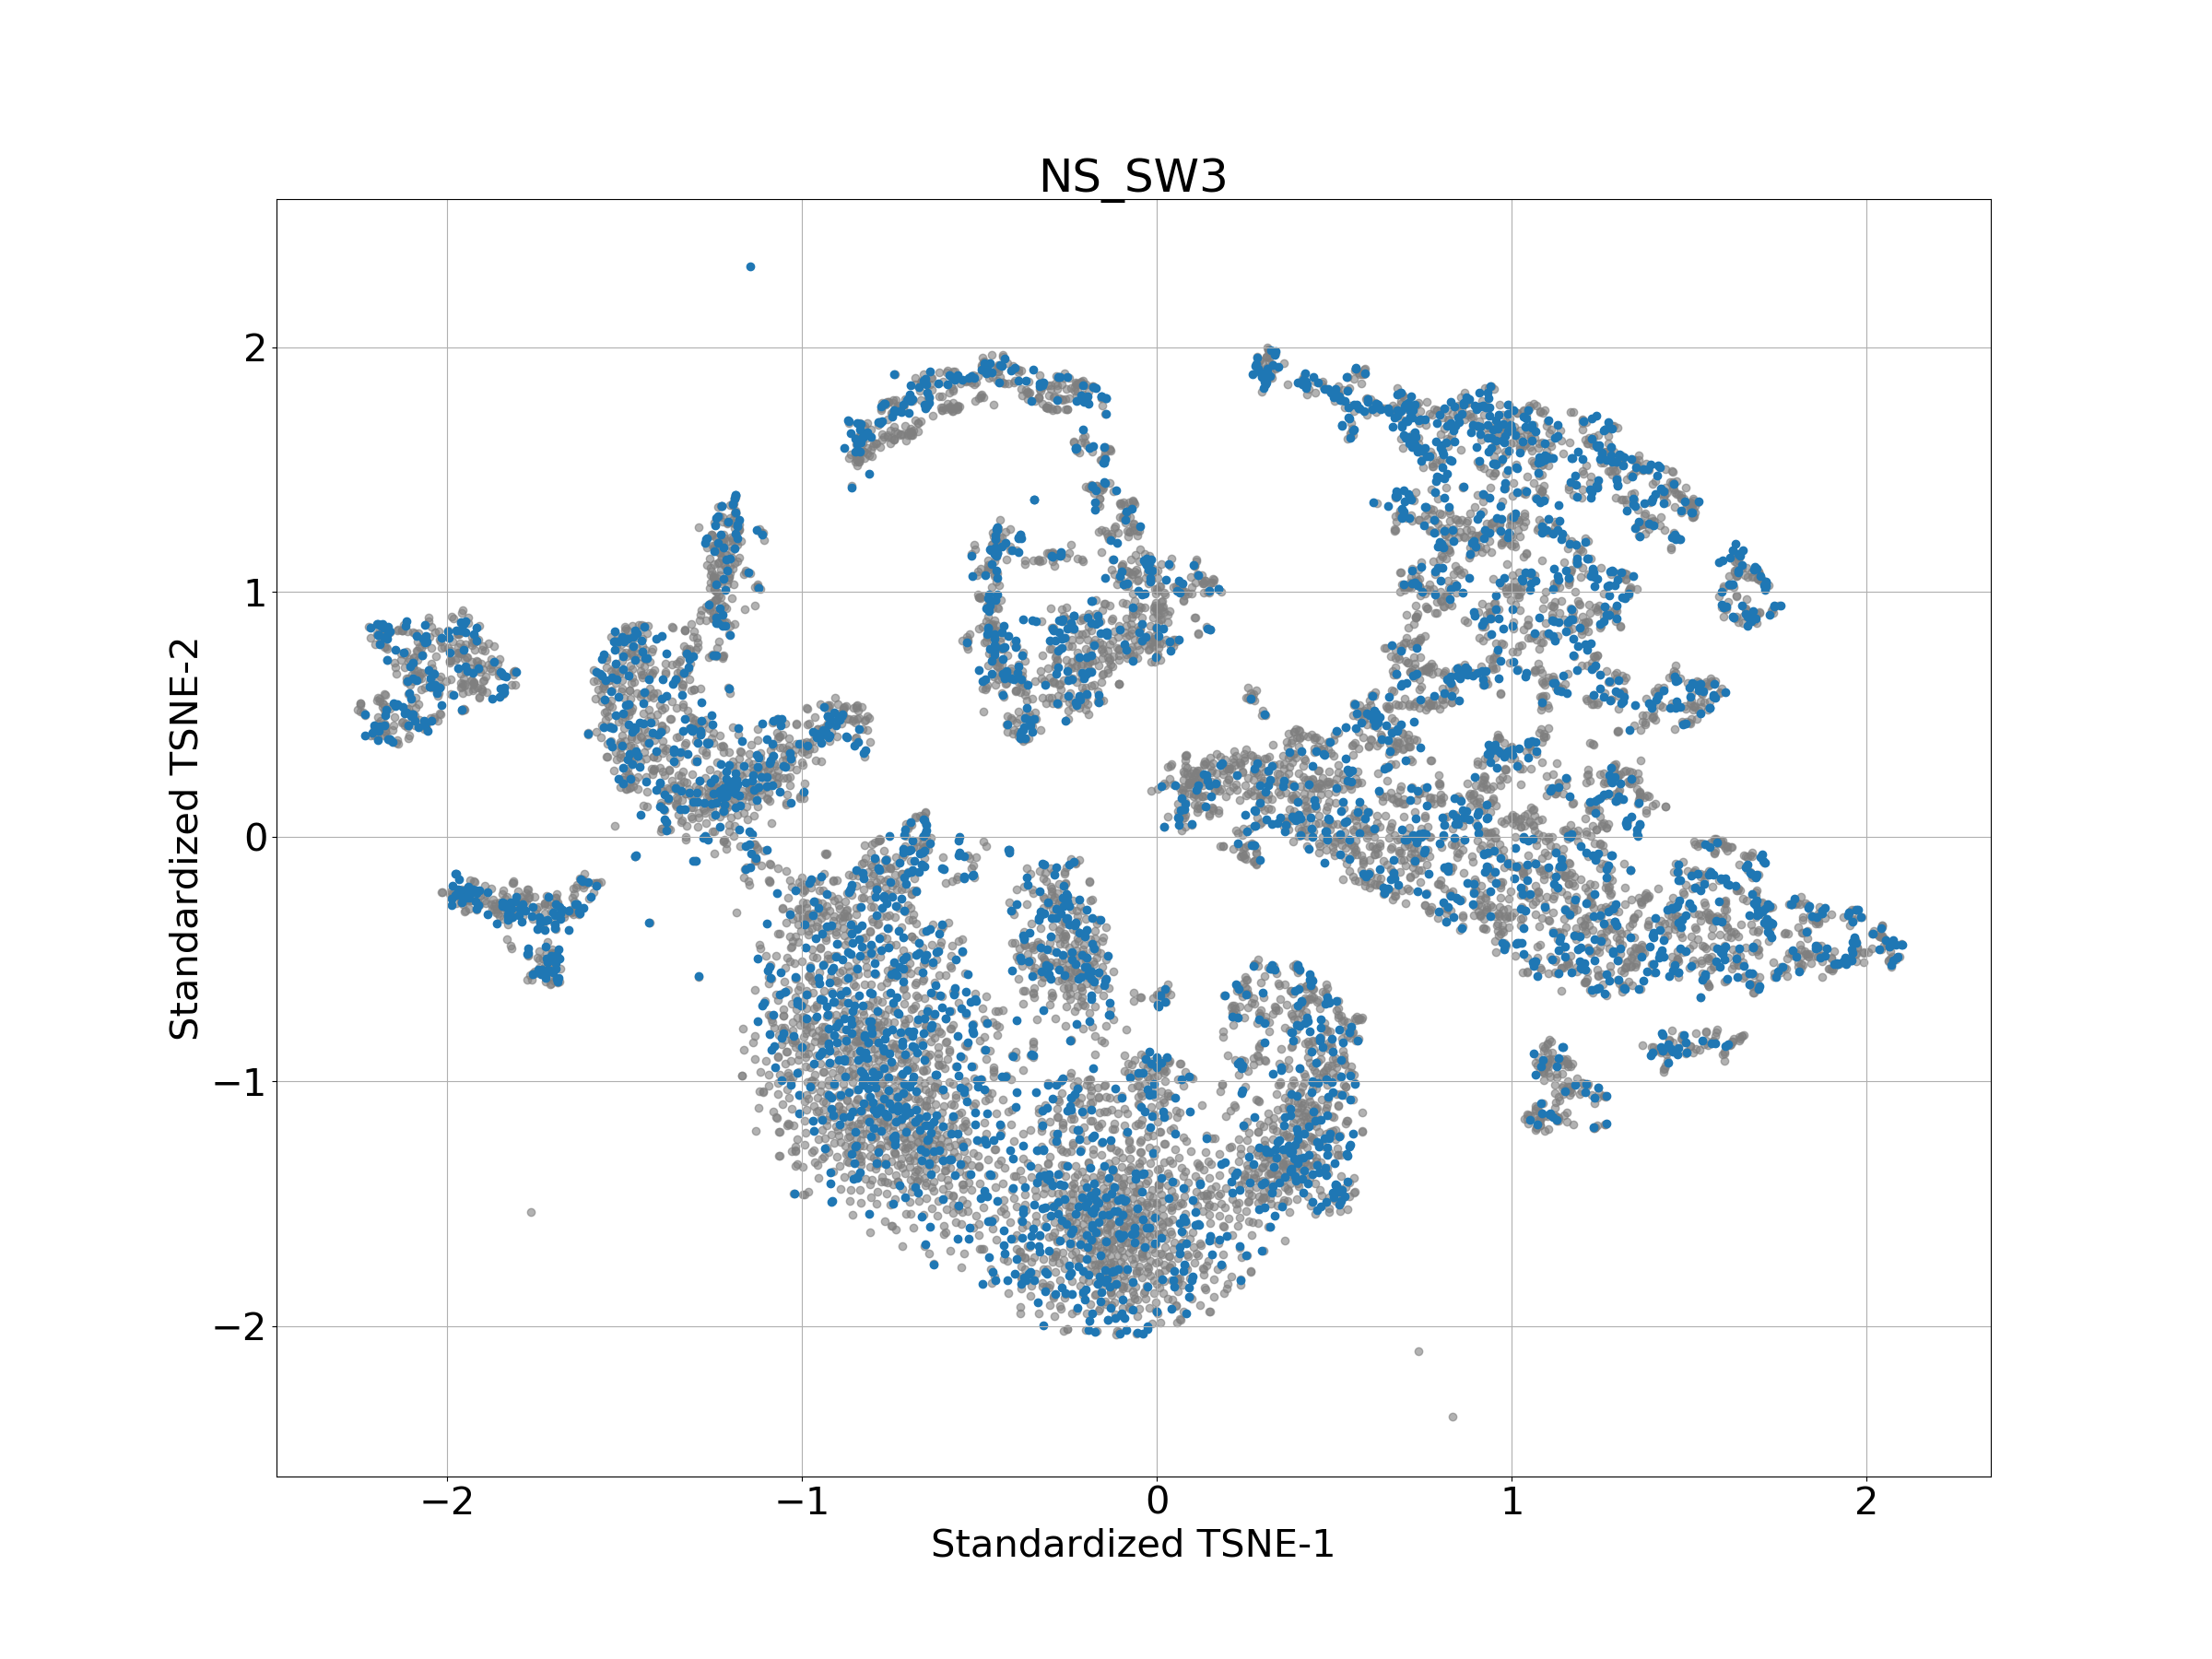
\includegraphics[height=5cm]{figures/TSNE/3.png}
                       &
                       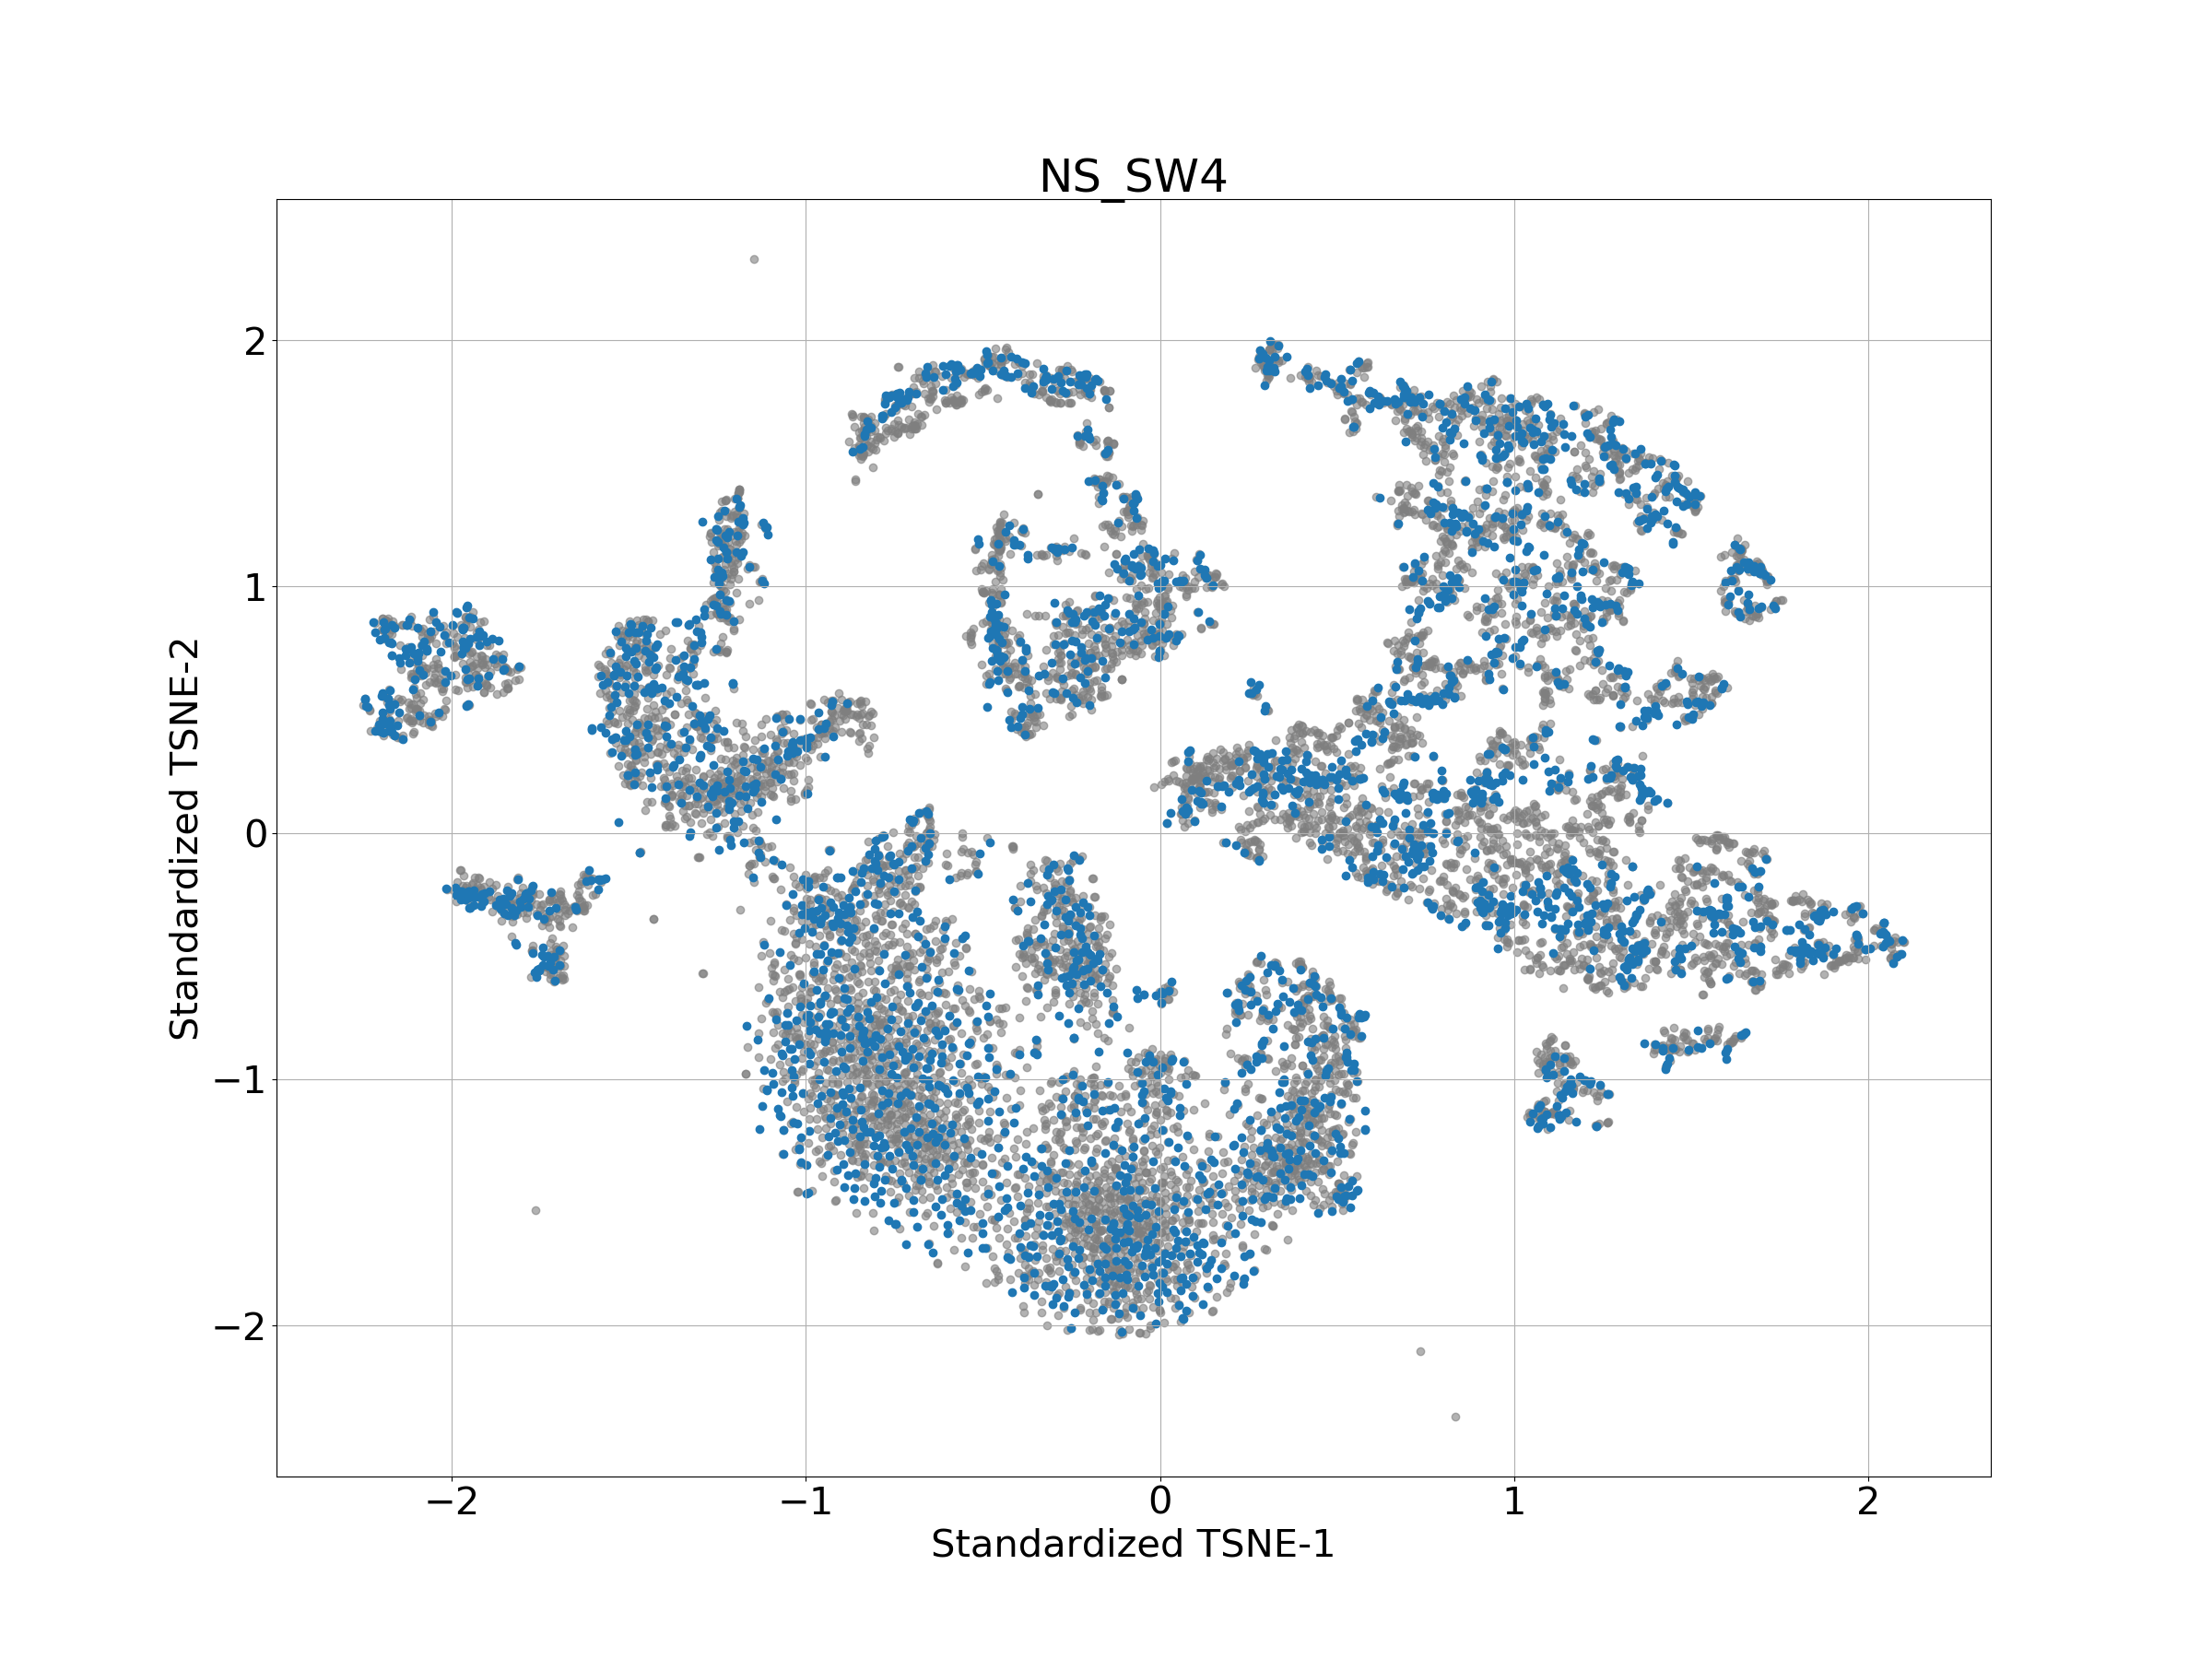
\includegraphics[height=5cm]{figures/TSNE/4.png}
                       \\
                    
                       \mbox{(c) NS\_SW3} & \mbox{(d) NS\_SW4} \\
                    \end{array}$
                \end{center}
                \caption{2D TSNE Plot of Each Samples}
                \label{fig:2dtsne}
            \end{figure}
        
        \subsection{TSNE Map in 3D}
            However, in figure \ref{fig:2dtsne}, I could not find linear tendency. I thought that was occurred by dimensional reduction, so I added one more axis to make 3D plot. The 3D TSNE map of each sample is in figure \ref{fig:3dtsne}.
            \begin{figure}[bph]
                \begin{center}
                    $\begin{array}{cc}
                        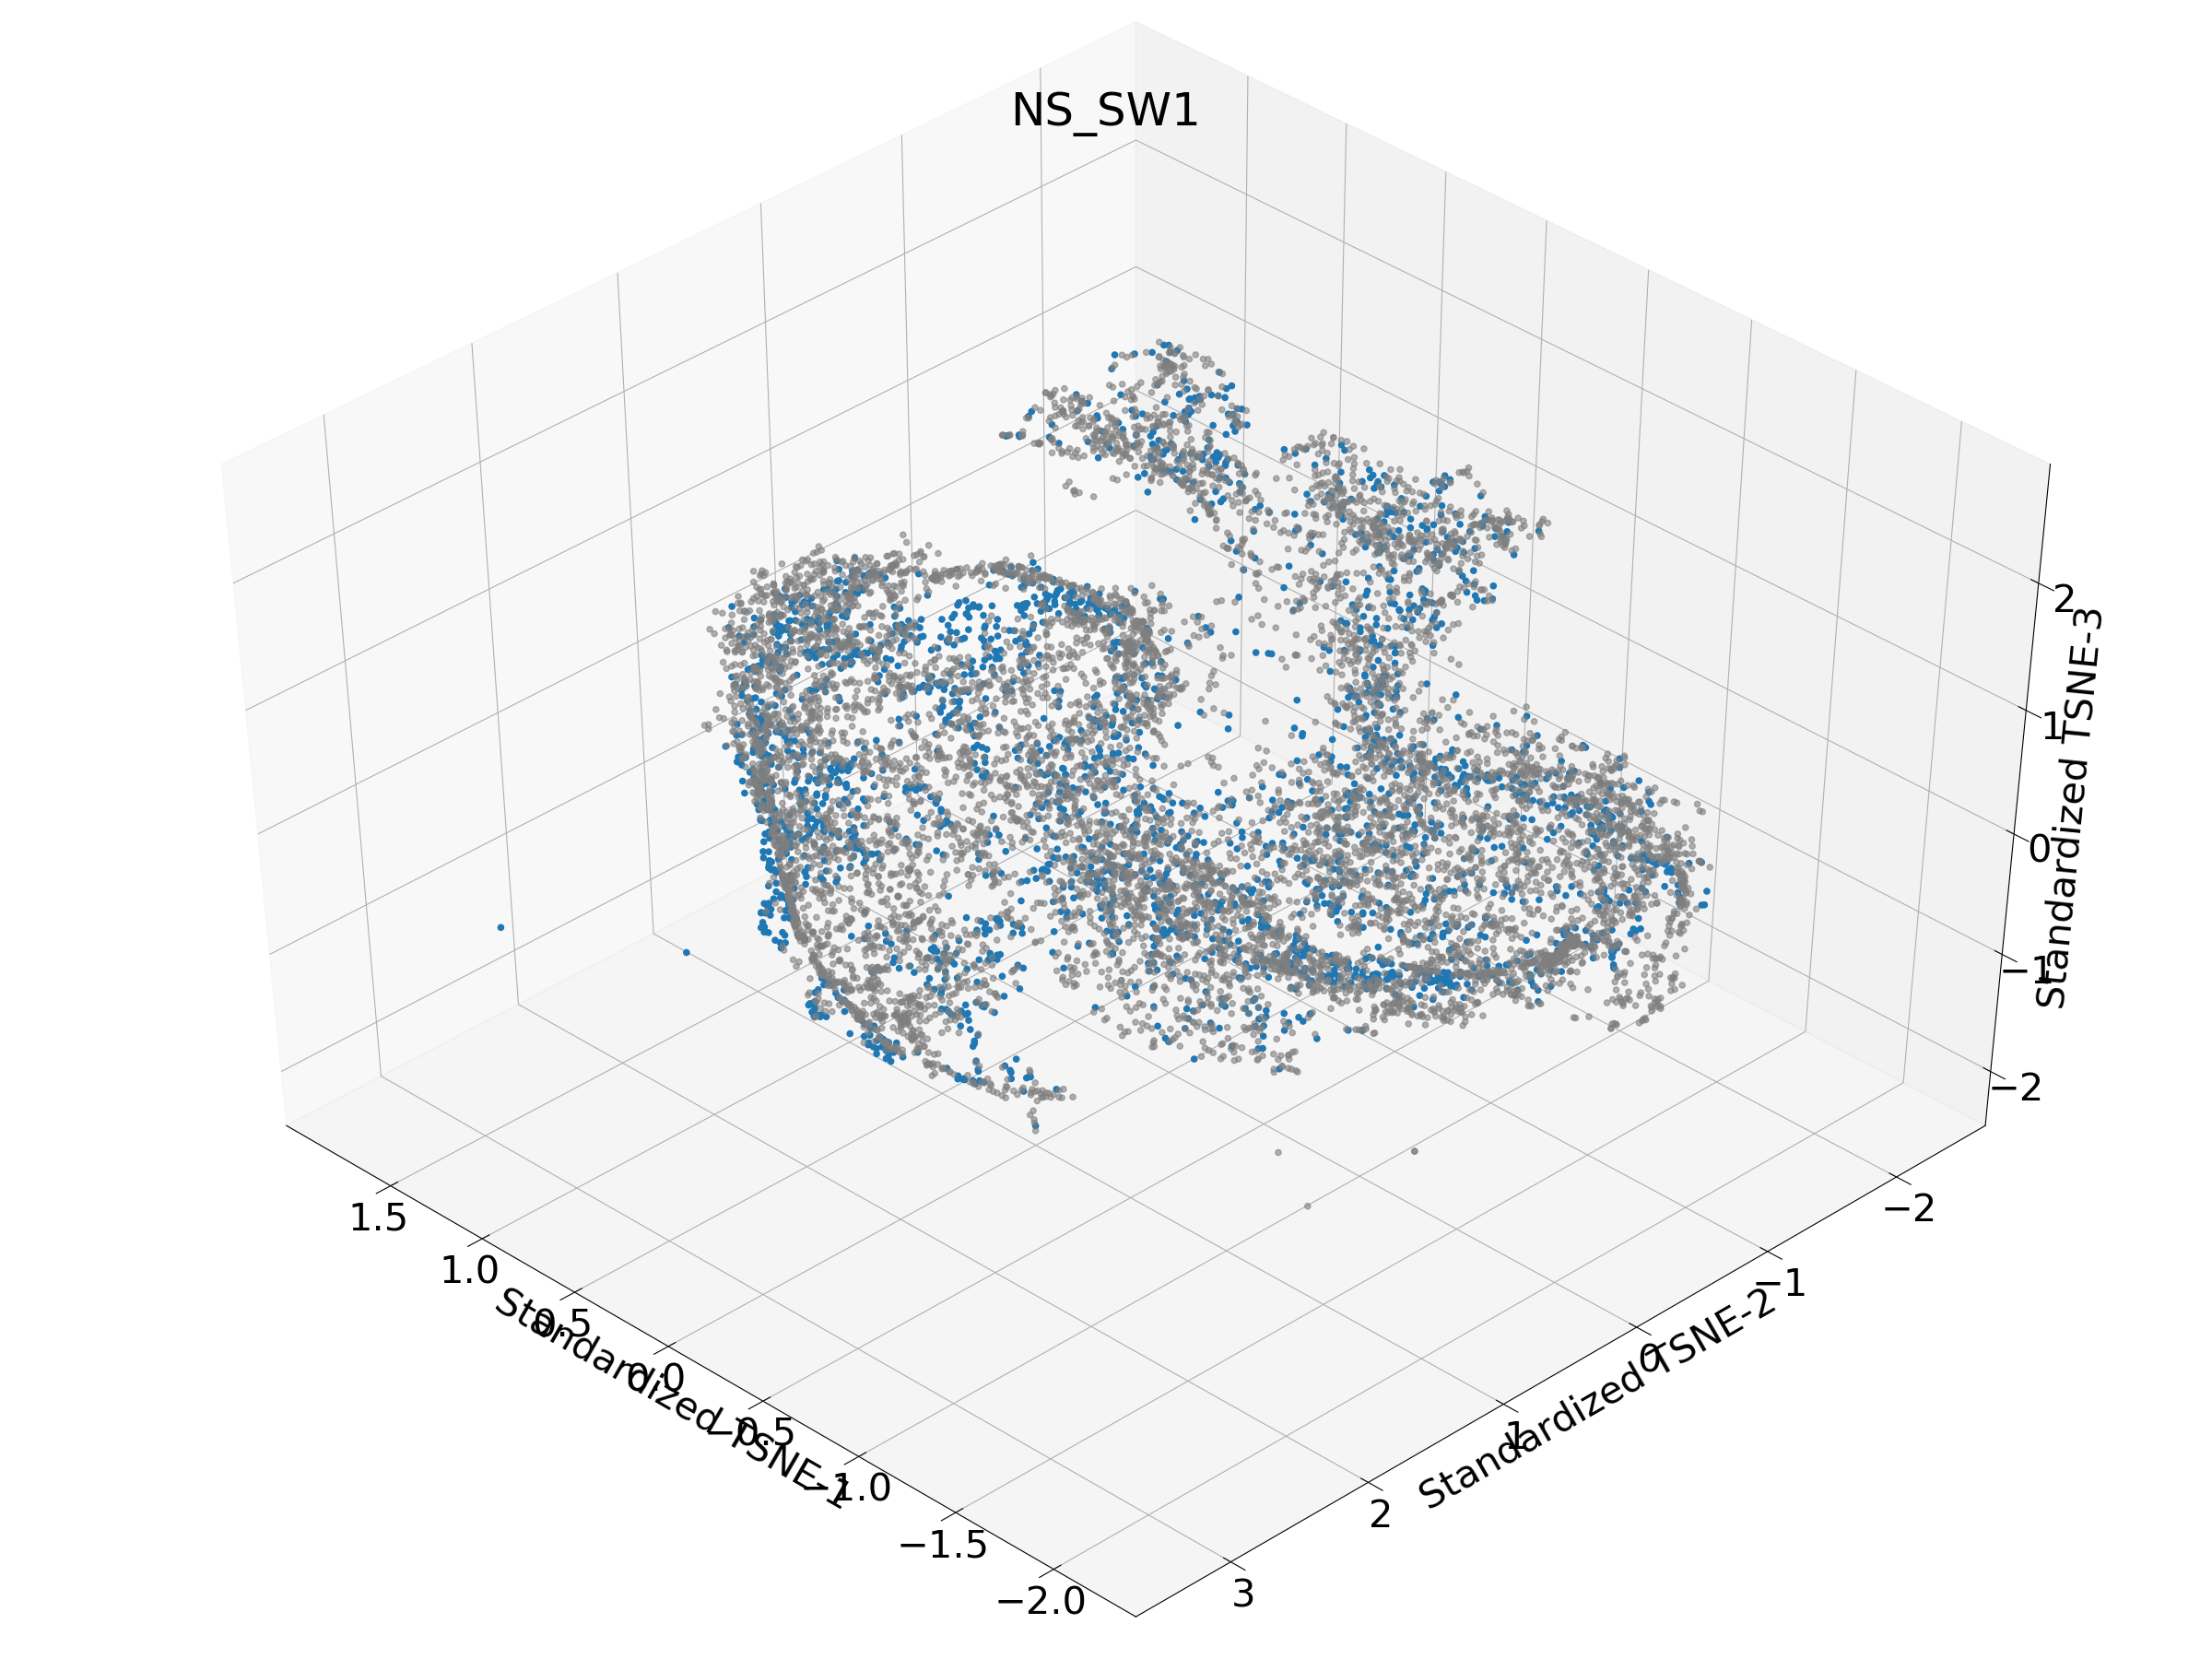
\includegraphics[height=5cm]{figures/TSNE3D/1.png}
                        &
                        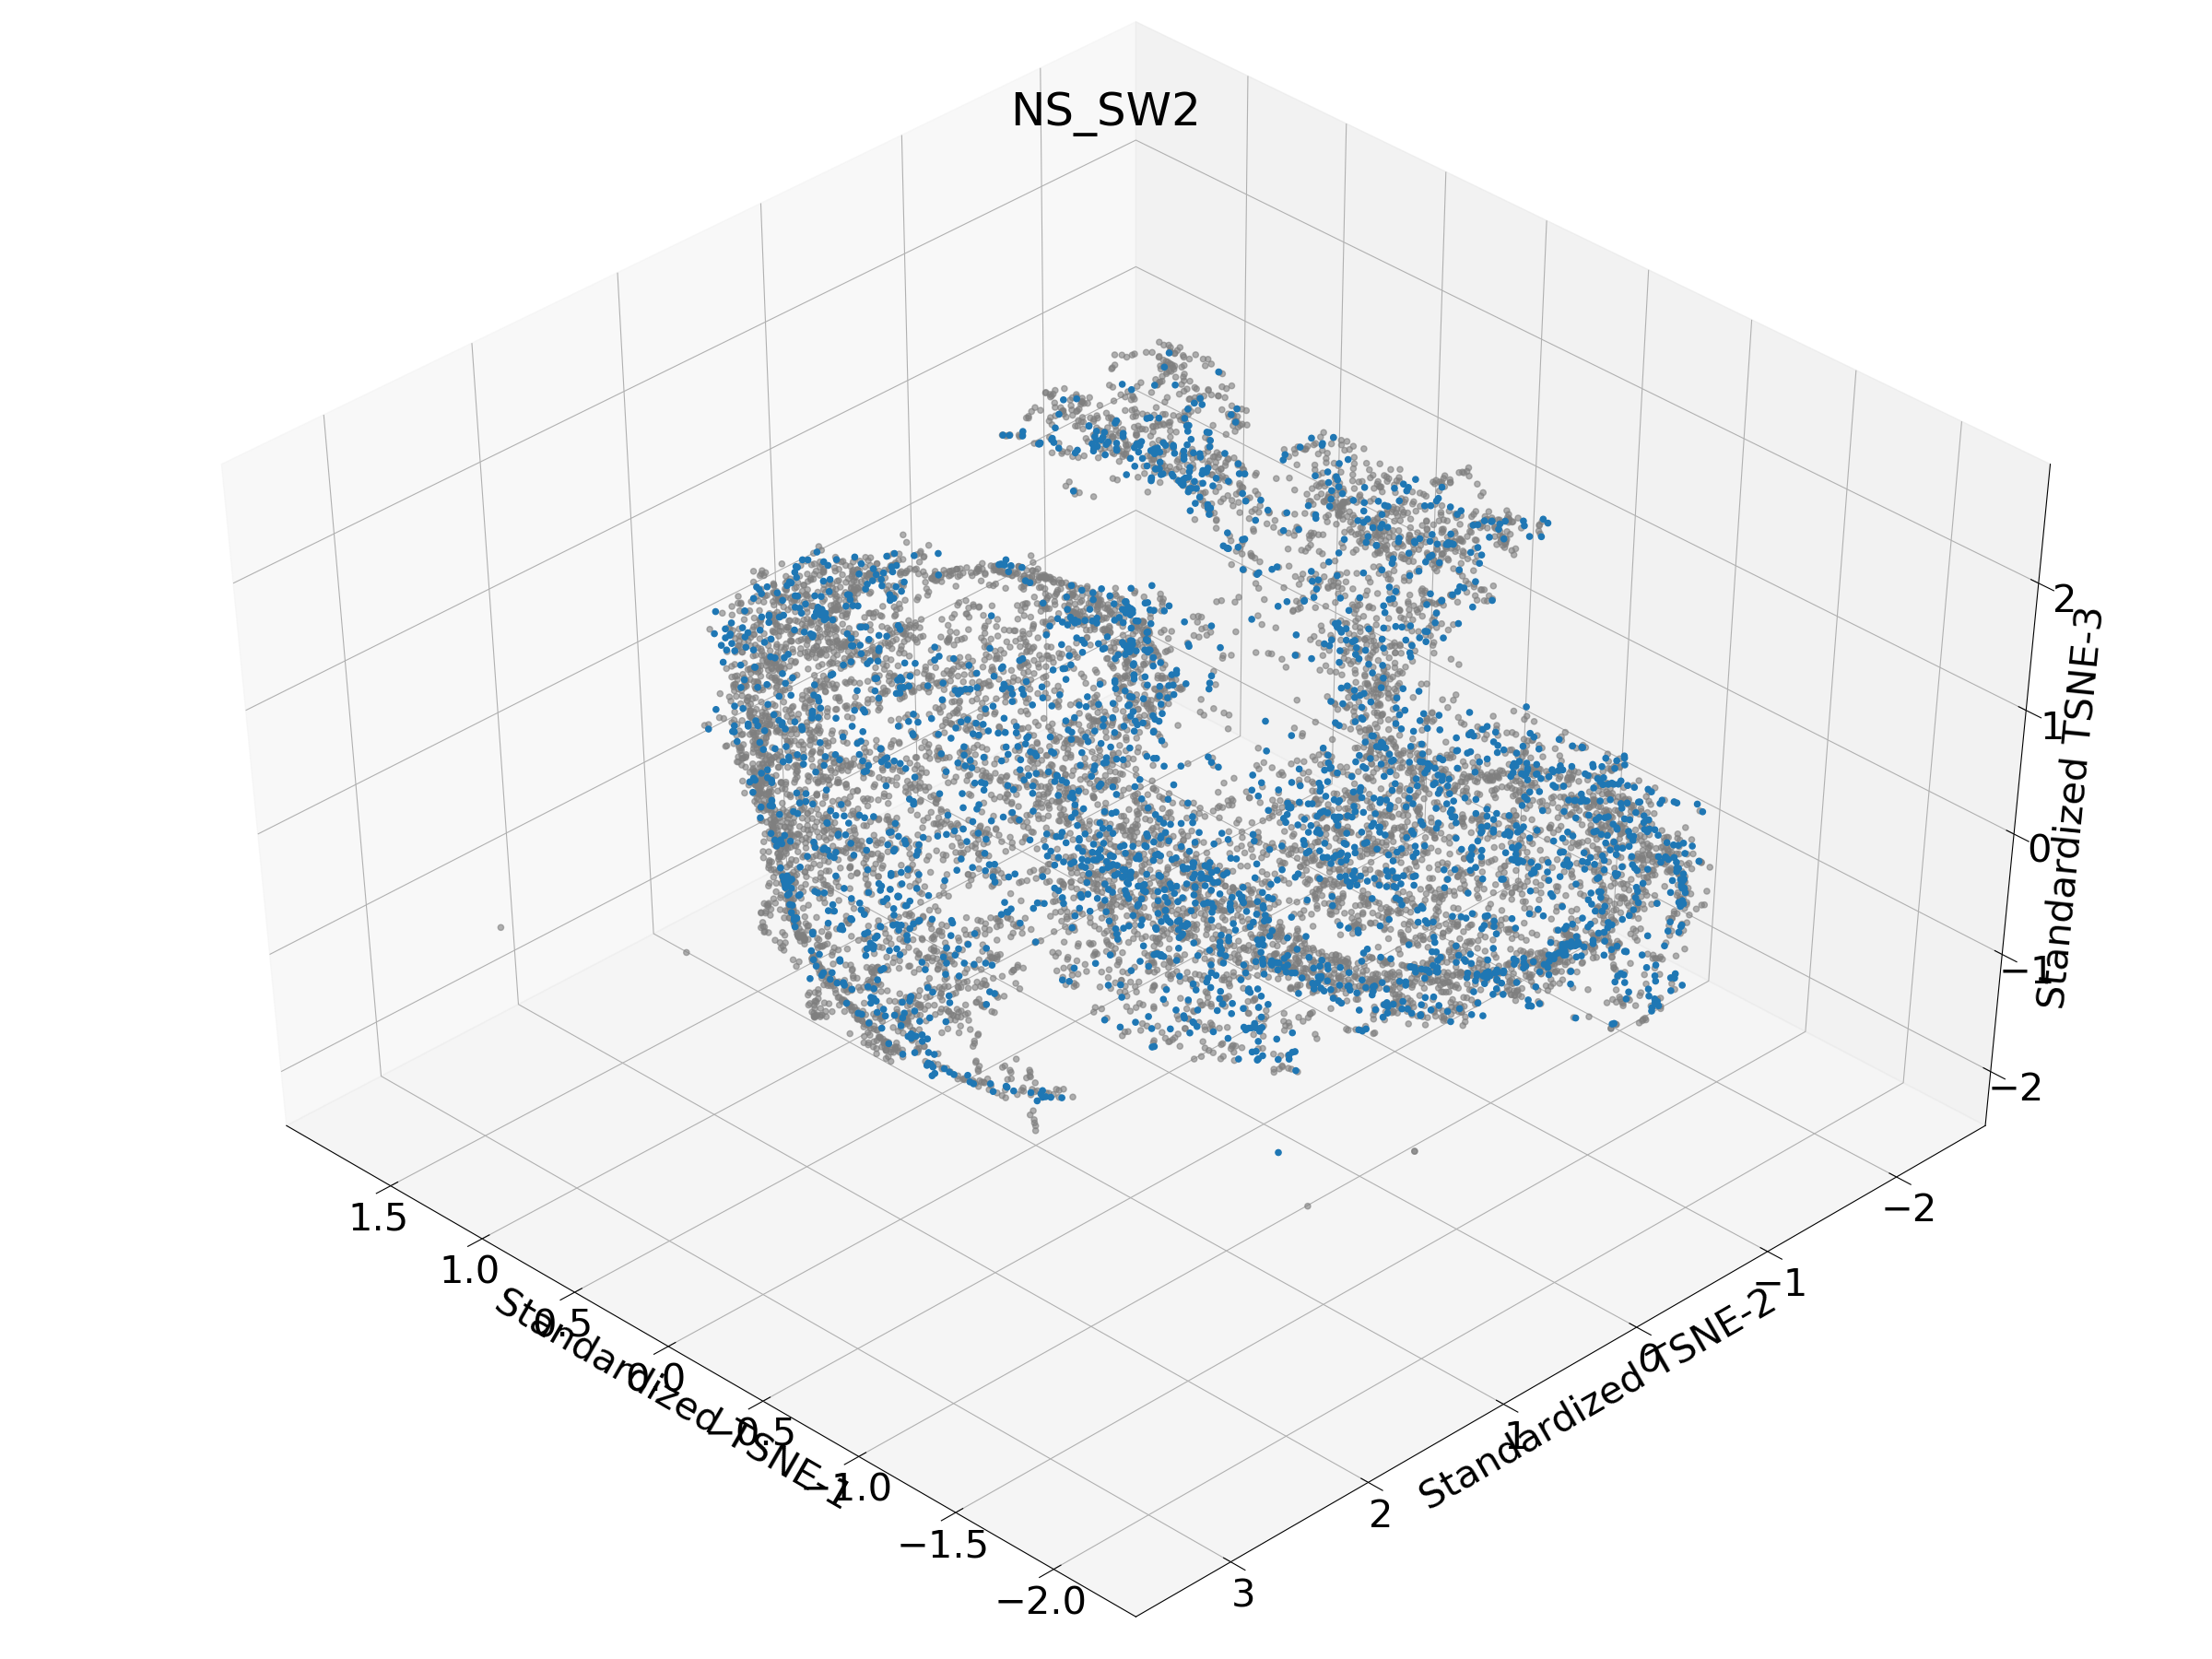
\includegraphics[height=5cm]{figures/TSNE3D/2.png}
                        \\
                        
                        \mbox{(a) NS\_SW1} & \mbox{(b) NS\_SW2} \\
                        
                        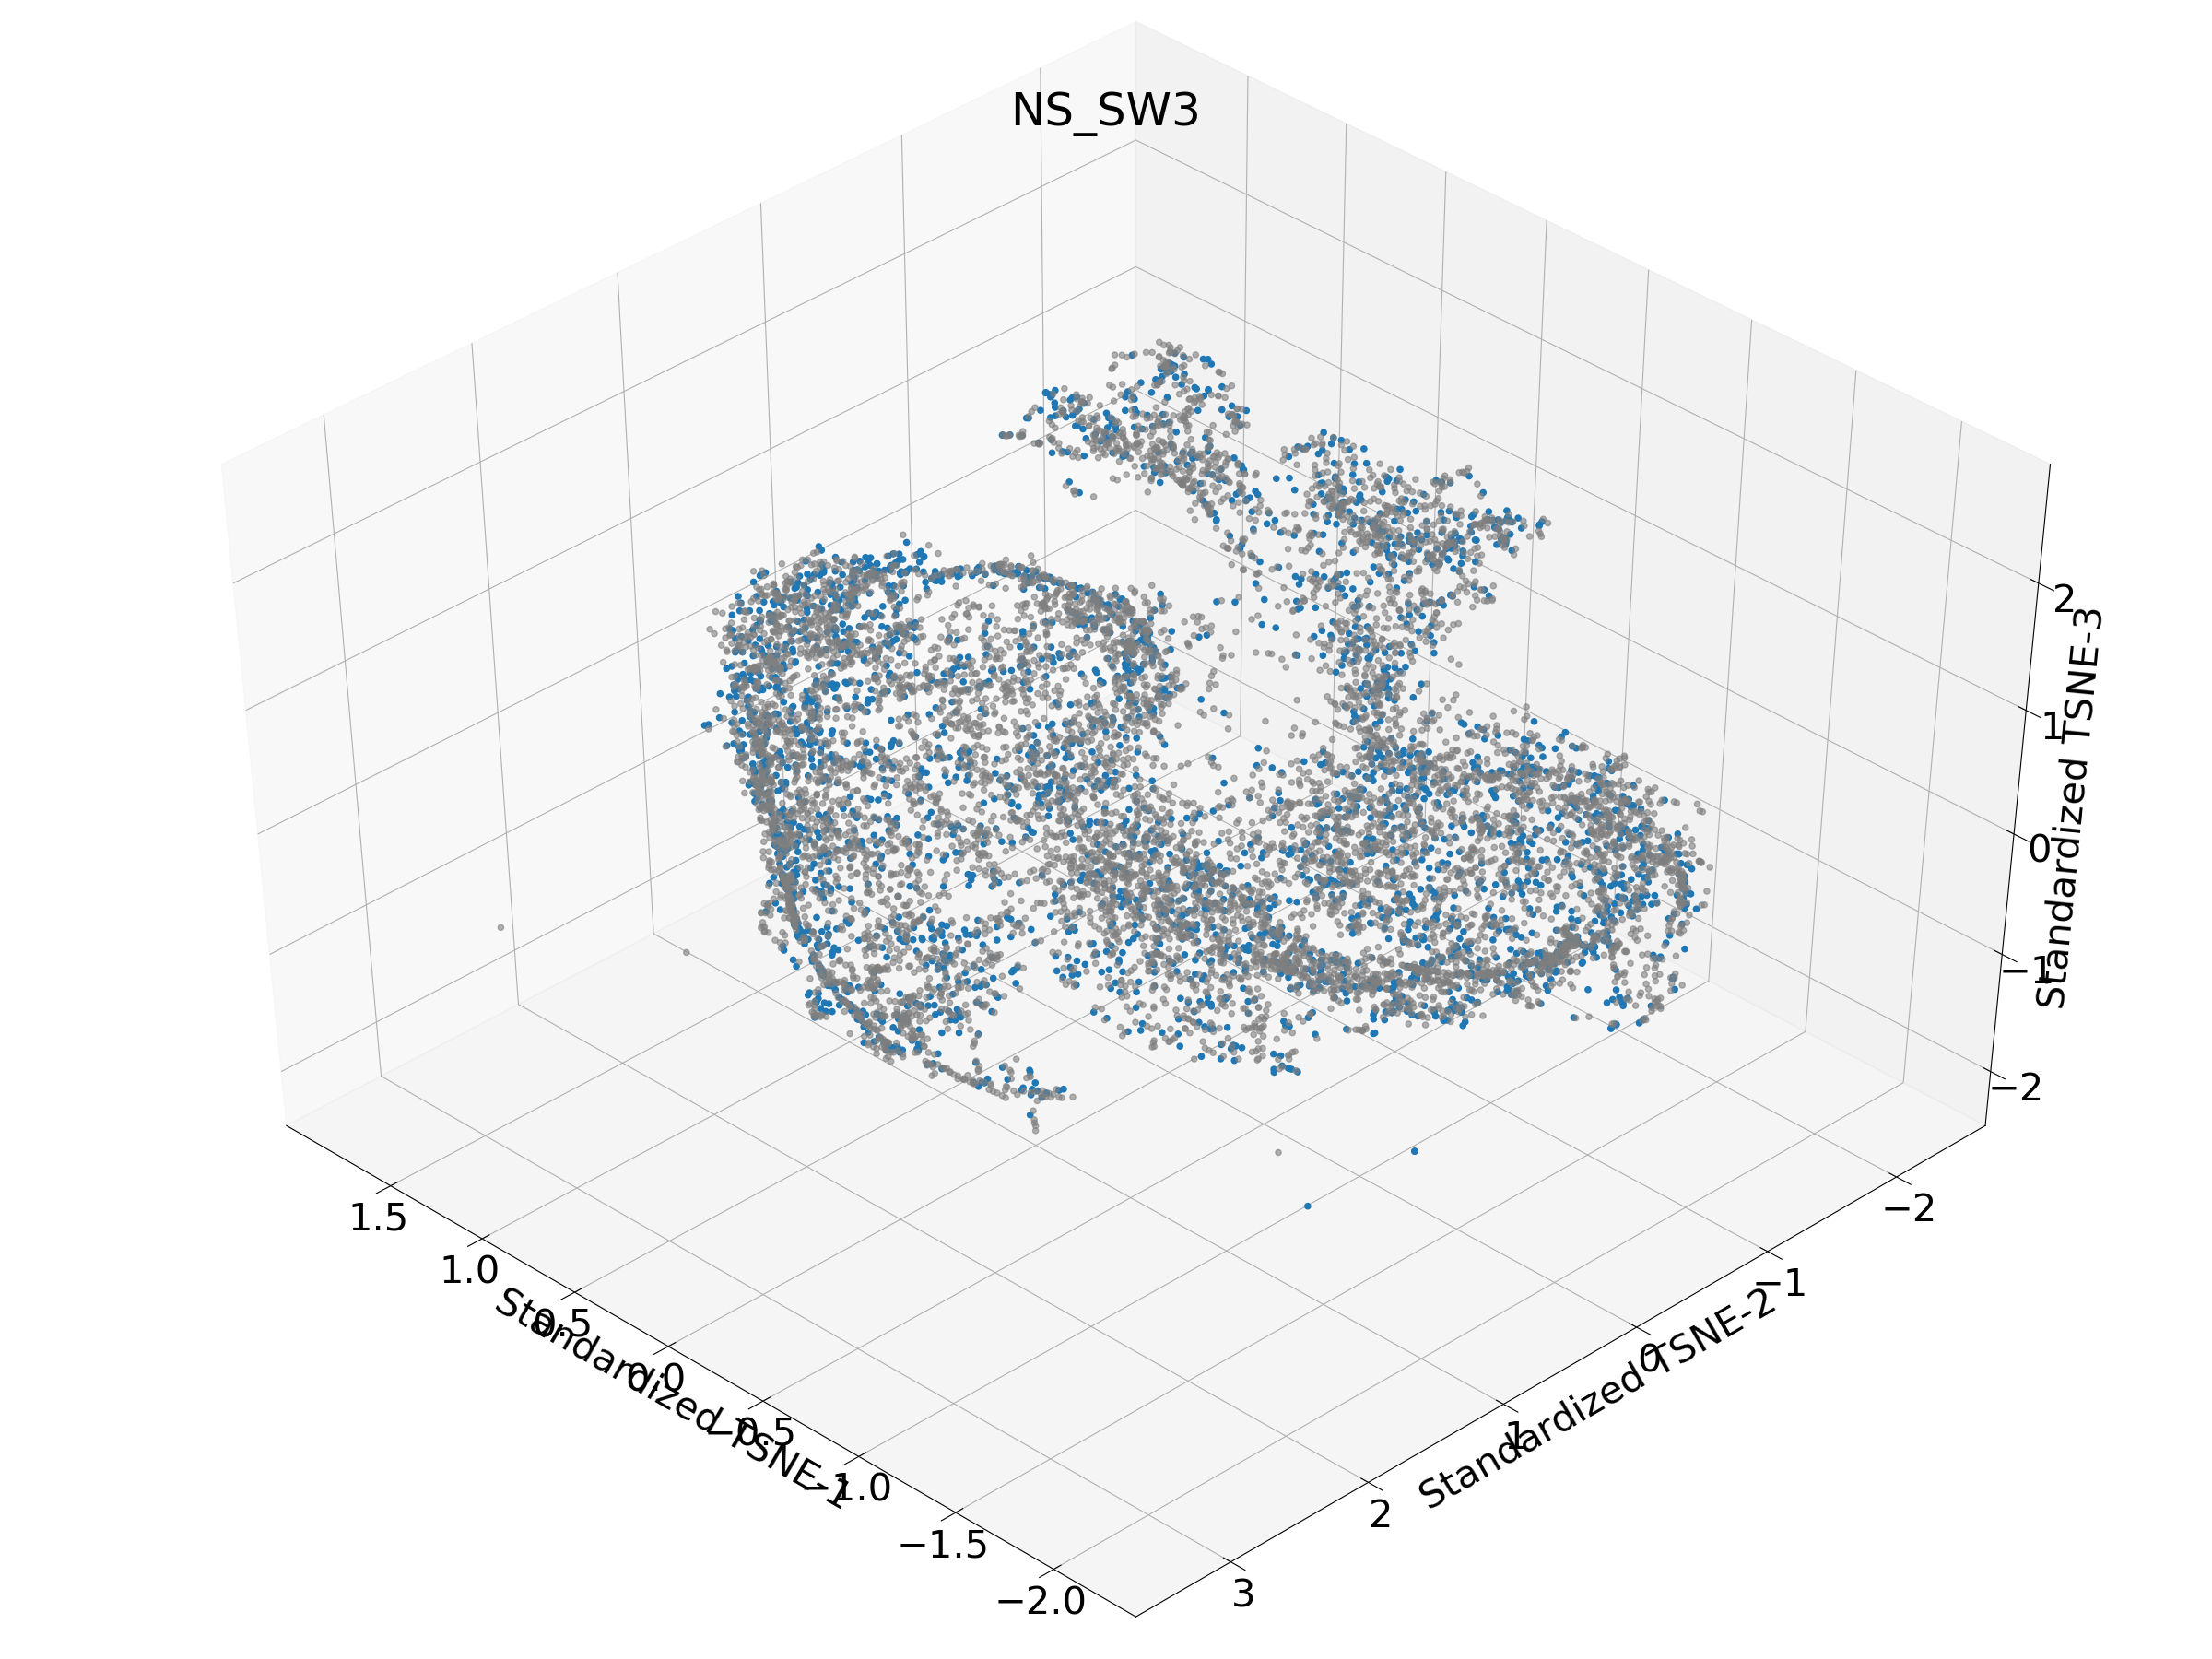
\includegraphics[height=5cm]{figures/TSNE3D/3.png}
                        &
                        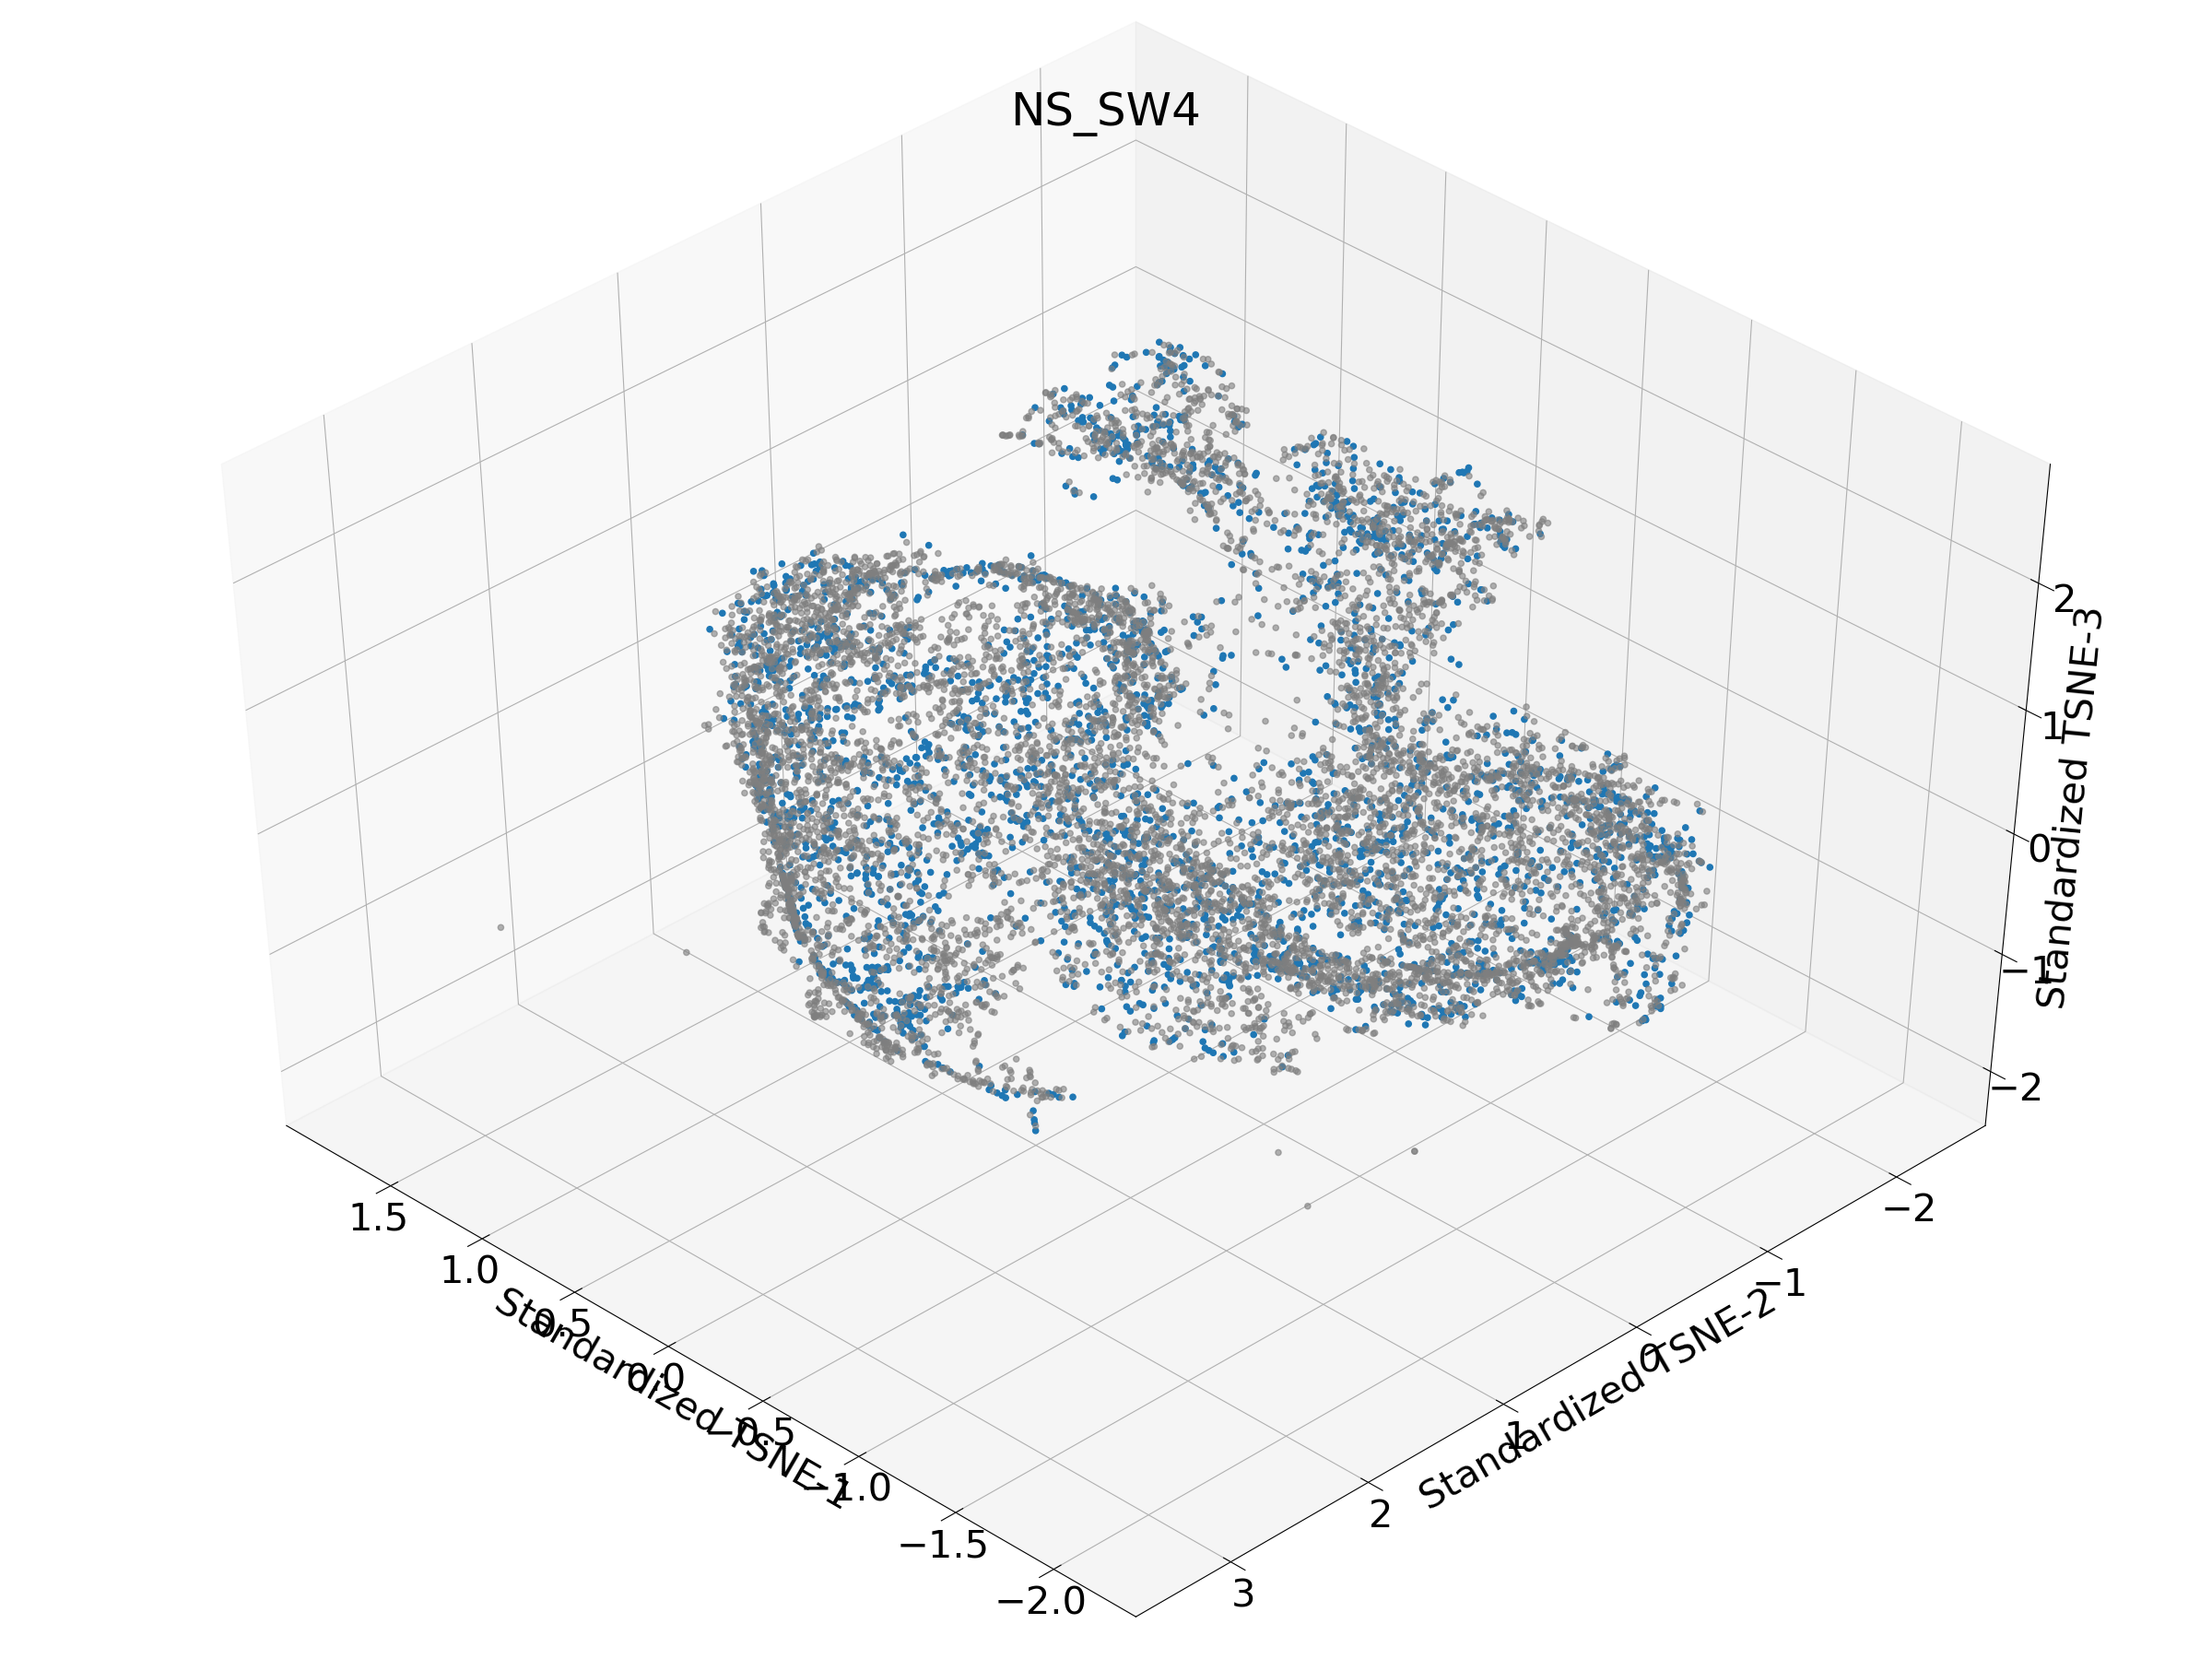
\includegraphics[height=5cm]{figures/TSNE3D/4.png}
                        \\
                        
                        \mbox{(c) NS\_SW3} & \mbox{(d) NS\_SW4} \\
                    \end{array}$
                \end{center}
                \label{fig:3dtsne}
                \caption{3D TSNE Plot of Each Samples}
            \end{figure} 
            You can also see data via URL in table \ref{tb:3dtsne}.
            \begin{table}[h!]
                \centering
                \caption{Table of URL of 3D TSNE}
                \label{tb:3dtsne}
                \begin{tabular}{c c}
                    Sample & URL \\ \hline
                    NS\_SW1 & \url{https://fumire.moe/made/IKJ_Lab/simple1.php} \\
                    NS\_SW2 & \url{https://fumire.moe/made/IKJ_Lab/simple2.php} \\
                    NS\_SW3 & \url{https://fumire.moe/made/IKJ_Lab/simple3.php} \\
                    NS\_SW4 & \url{https://fumire.moe/made/IKJ_Lab/simple4.php} \\
                \end{tabular}
            \end{table}
        
        \subsection{Clustering with KMeans Algorithm}
            Amongst many clustering algorithm, I chose KMeans algorithm. Because the hyper-parameter of KMeans algorithm is a number of groups, so the result can be intuitive. 
            The results of Kmeans algorithm are in figure \ref{fig:kmeans}. Also, you may see data via URL in table \ref{tb:cluster}.
            \begin{figure}[hbp]
                \begin{center}
                    $\begin{array}{cc}
                        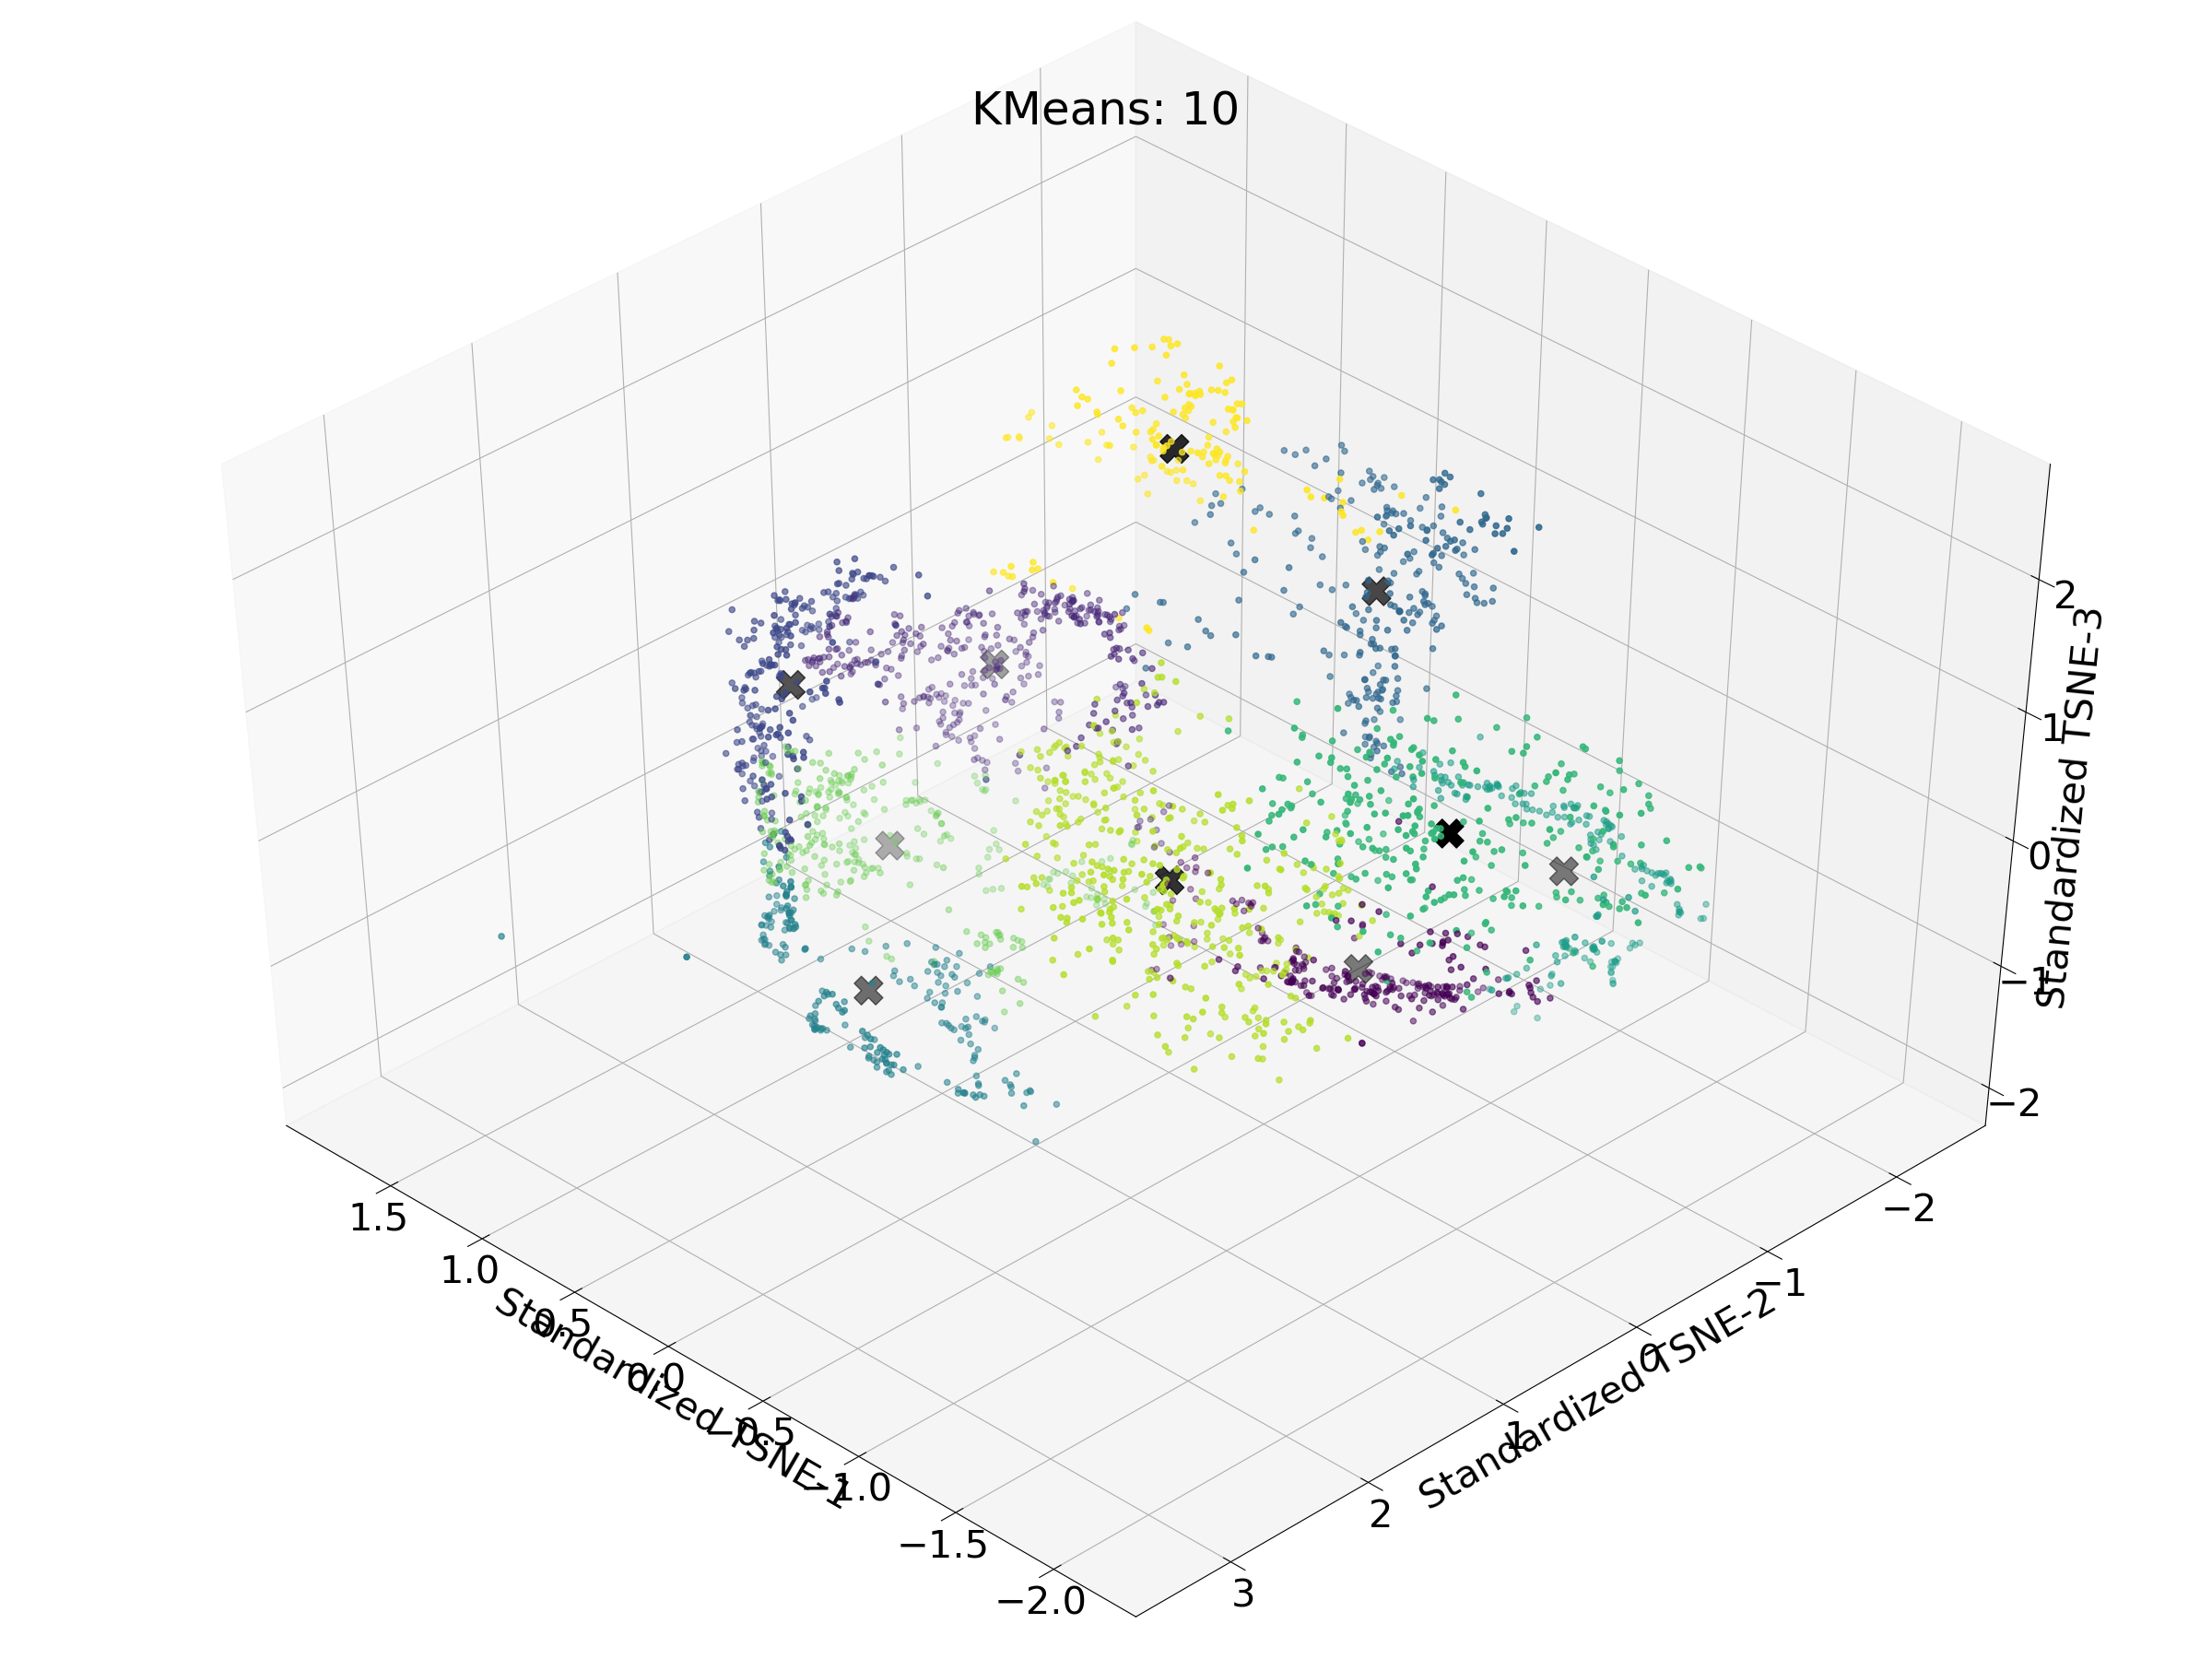
\includegraphics[height=5cm]{figures/KMeans/1.png}
                        &
                        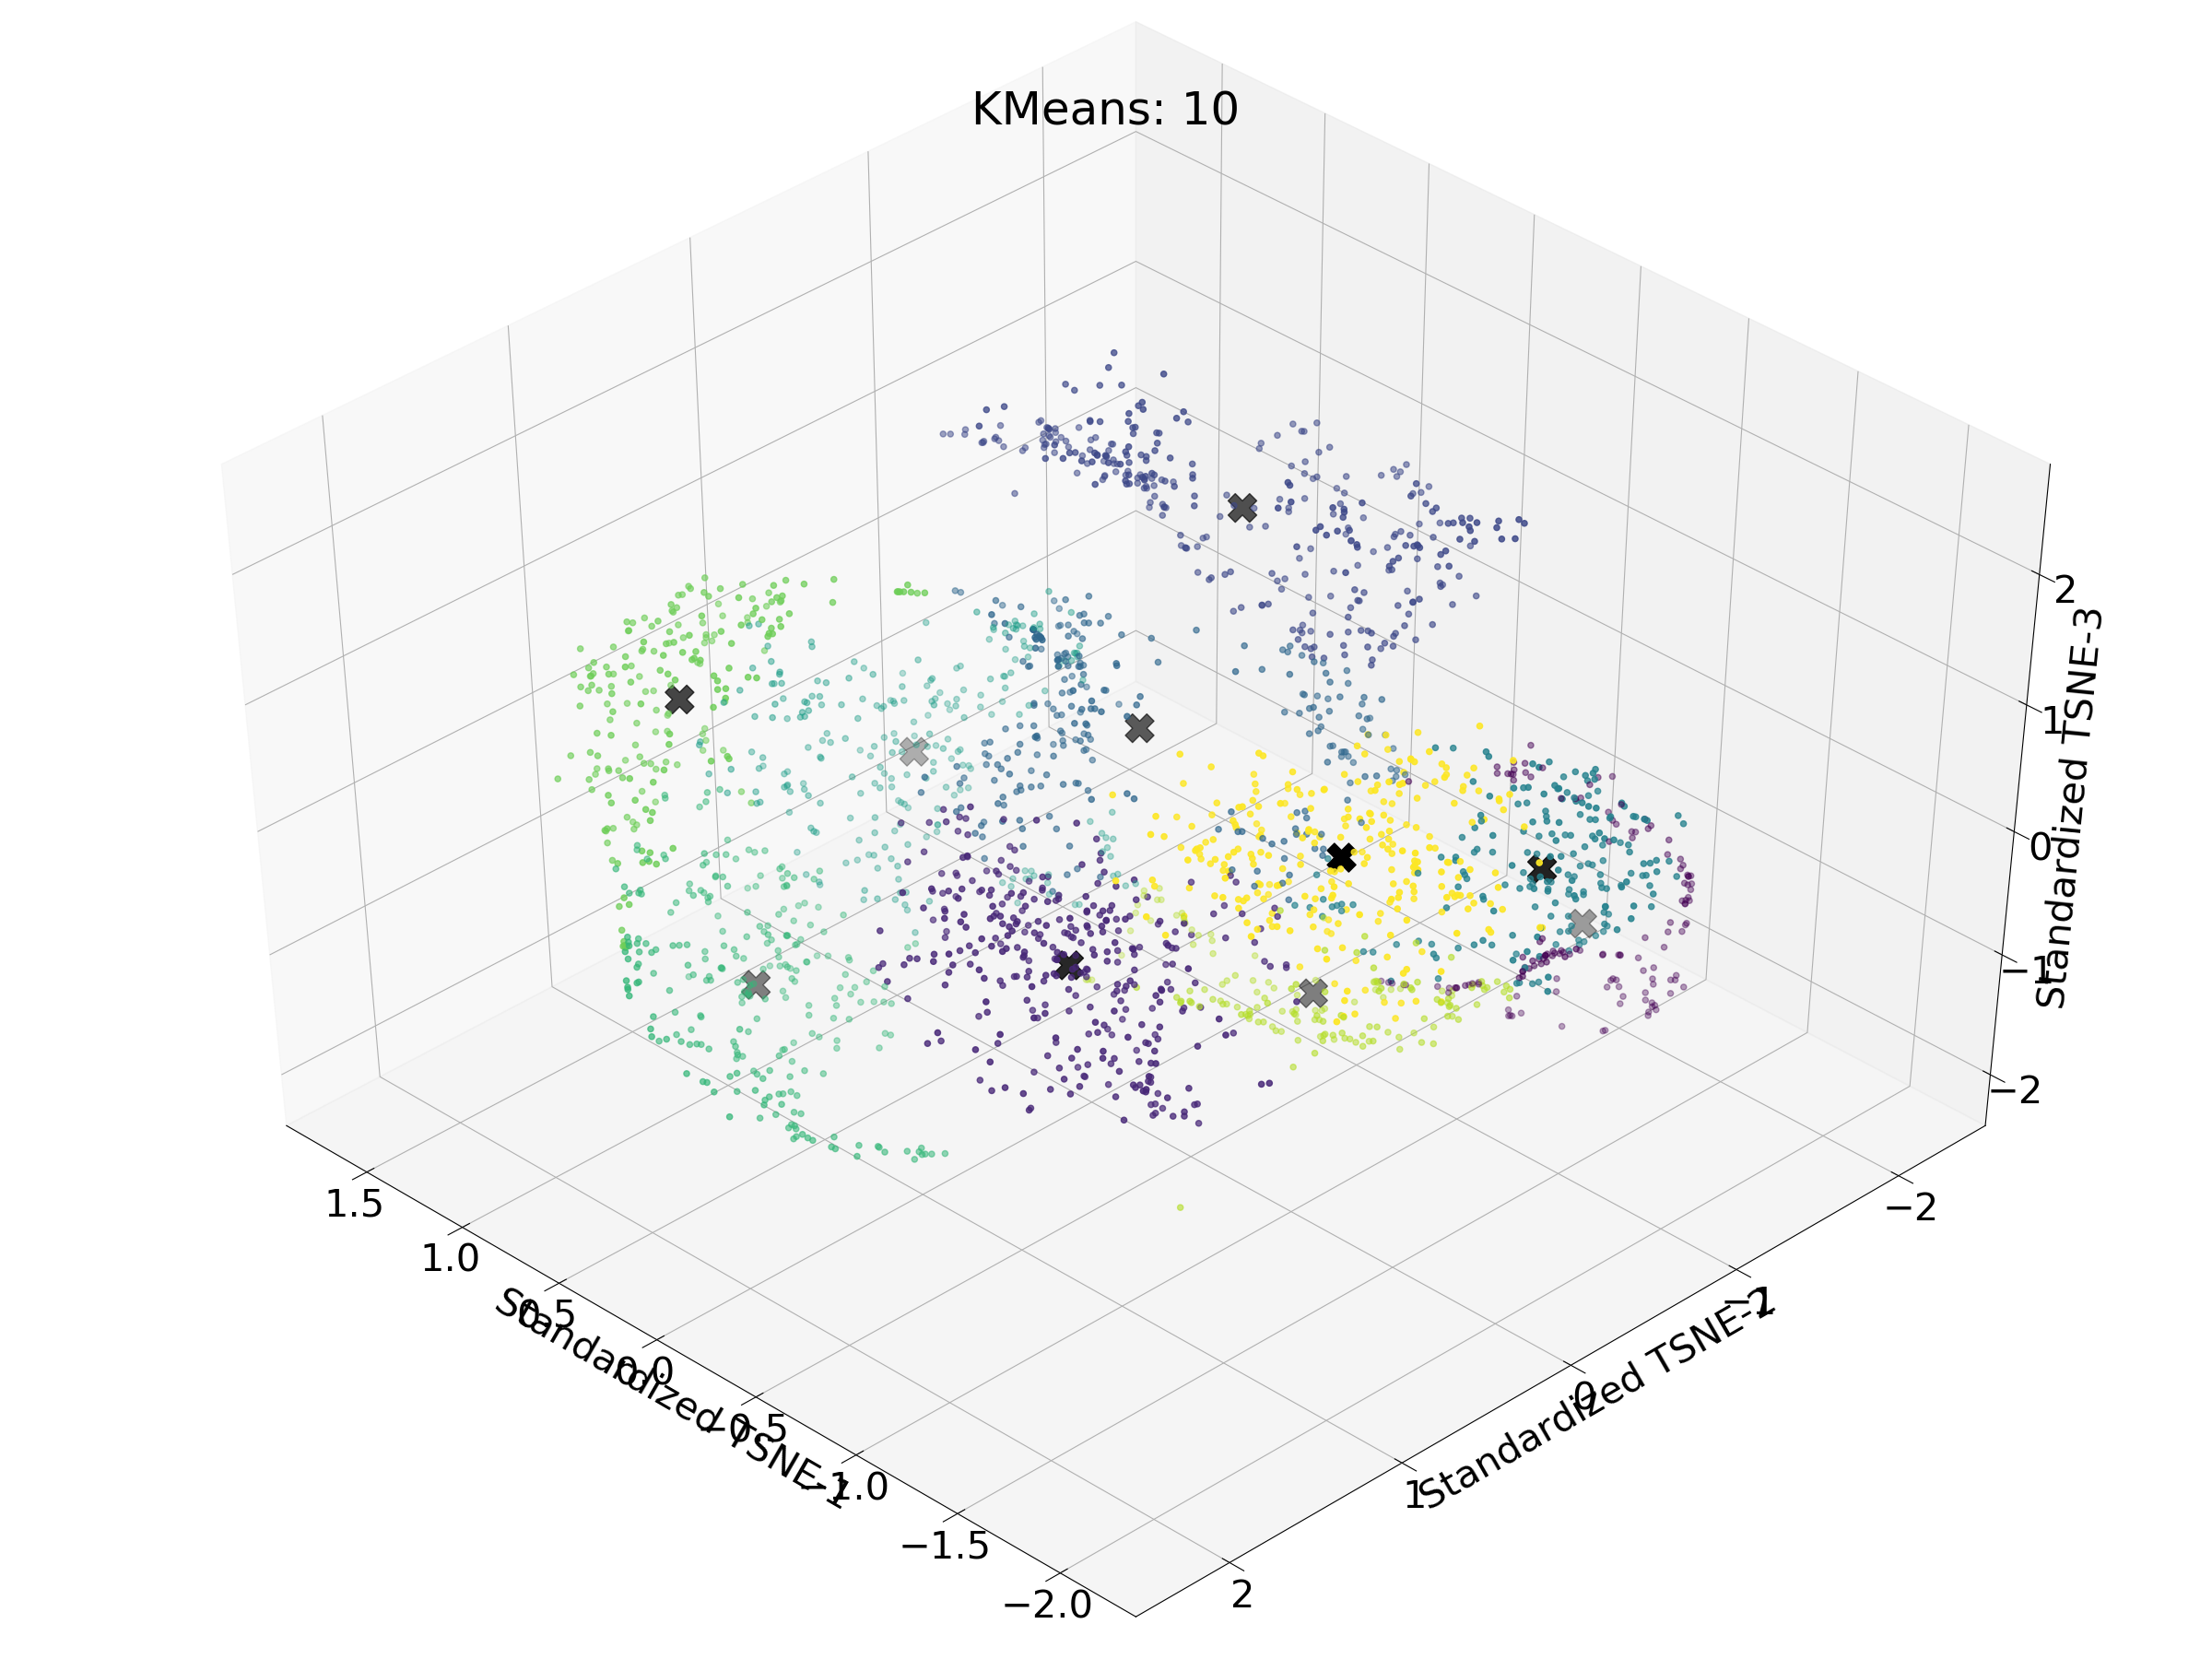
\includegraphics[height=5cm]{figures/KMeans/2.png}
                        \\
                        
                        \mbox{(a) NS\_SW1} & \mbox{(b) NS\_SW2} \\
                        
                        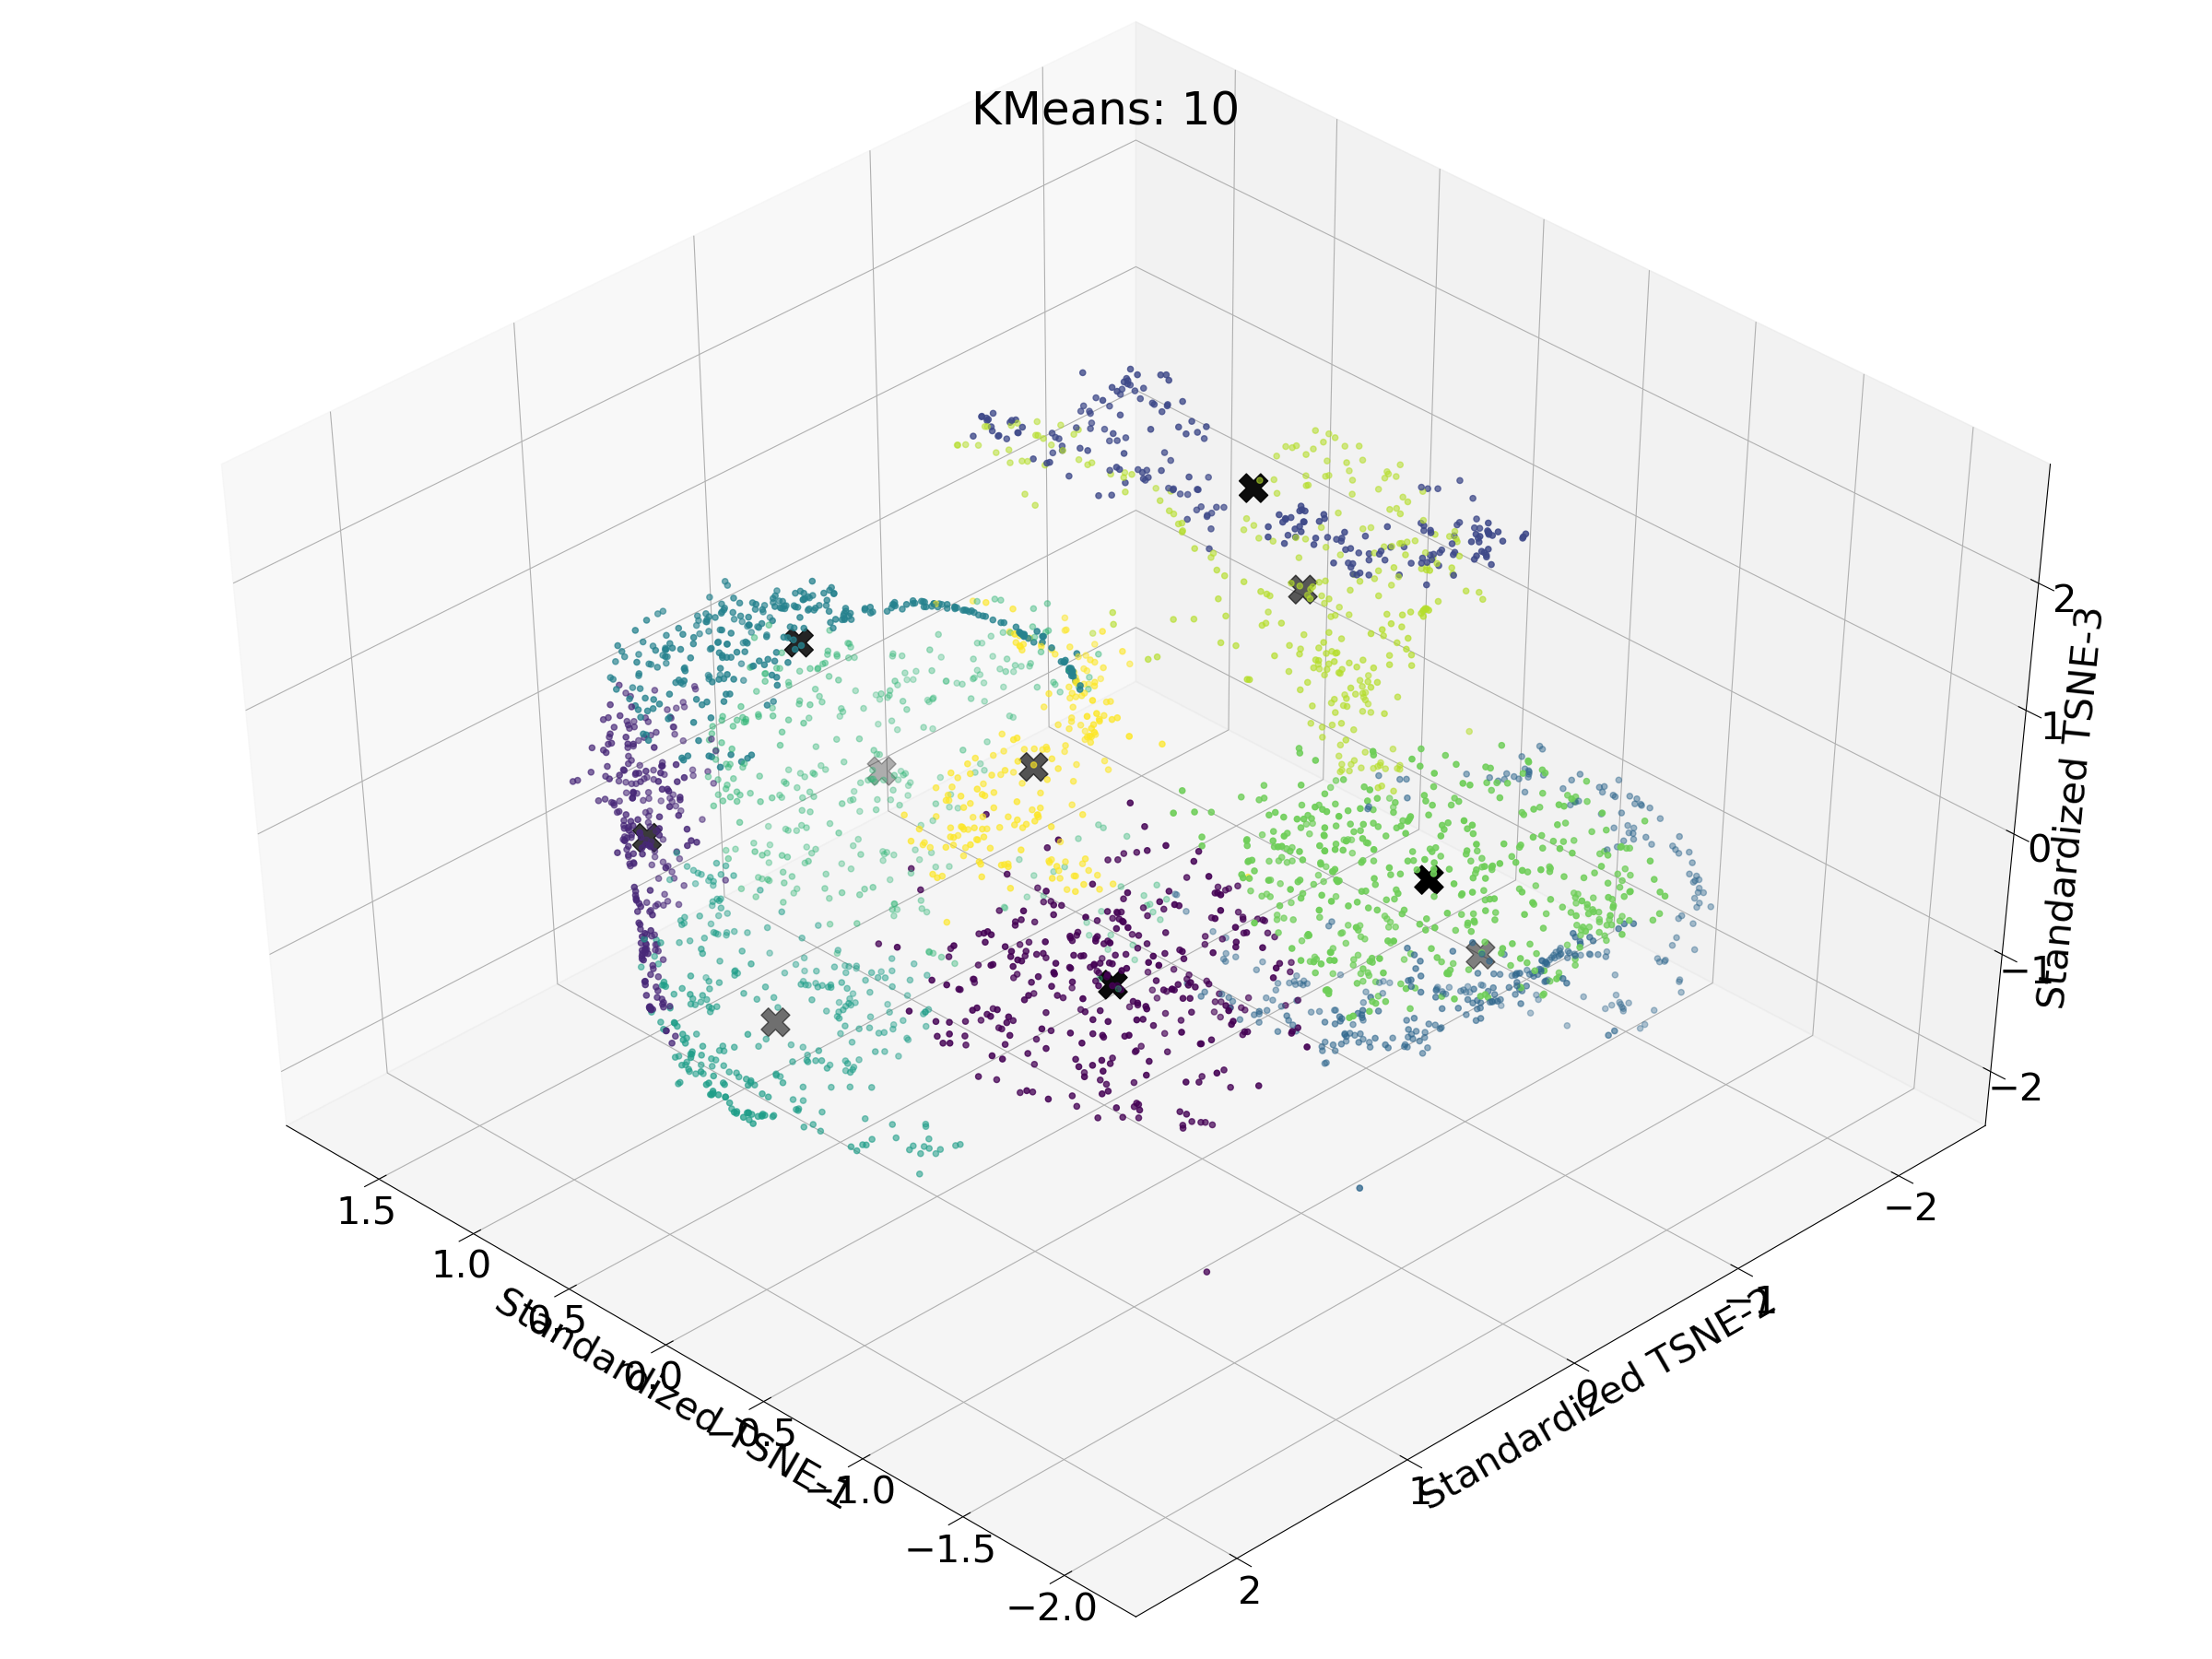
\includegraphics[height=5cm]{figures/KMeans/3.png}
                        &
                        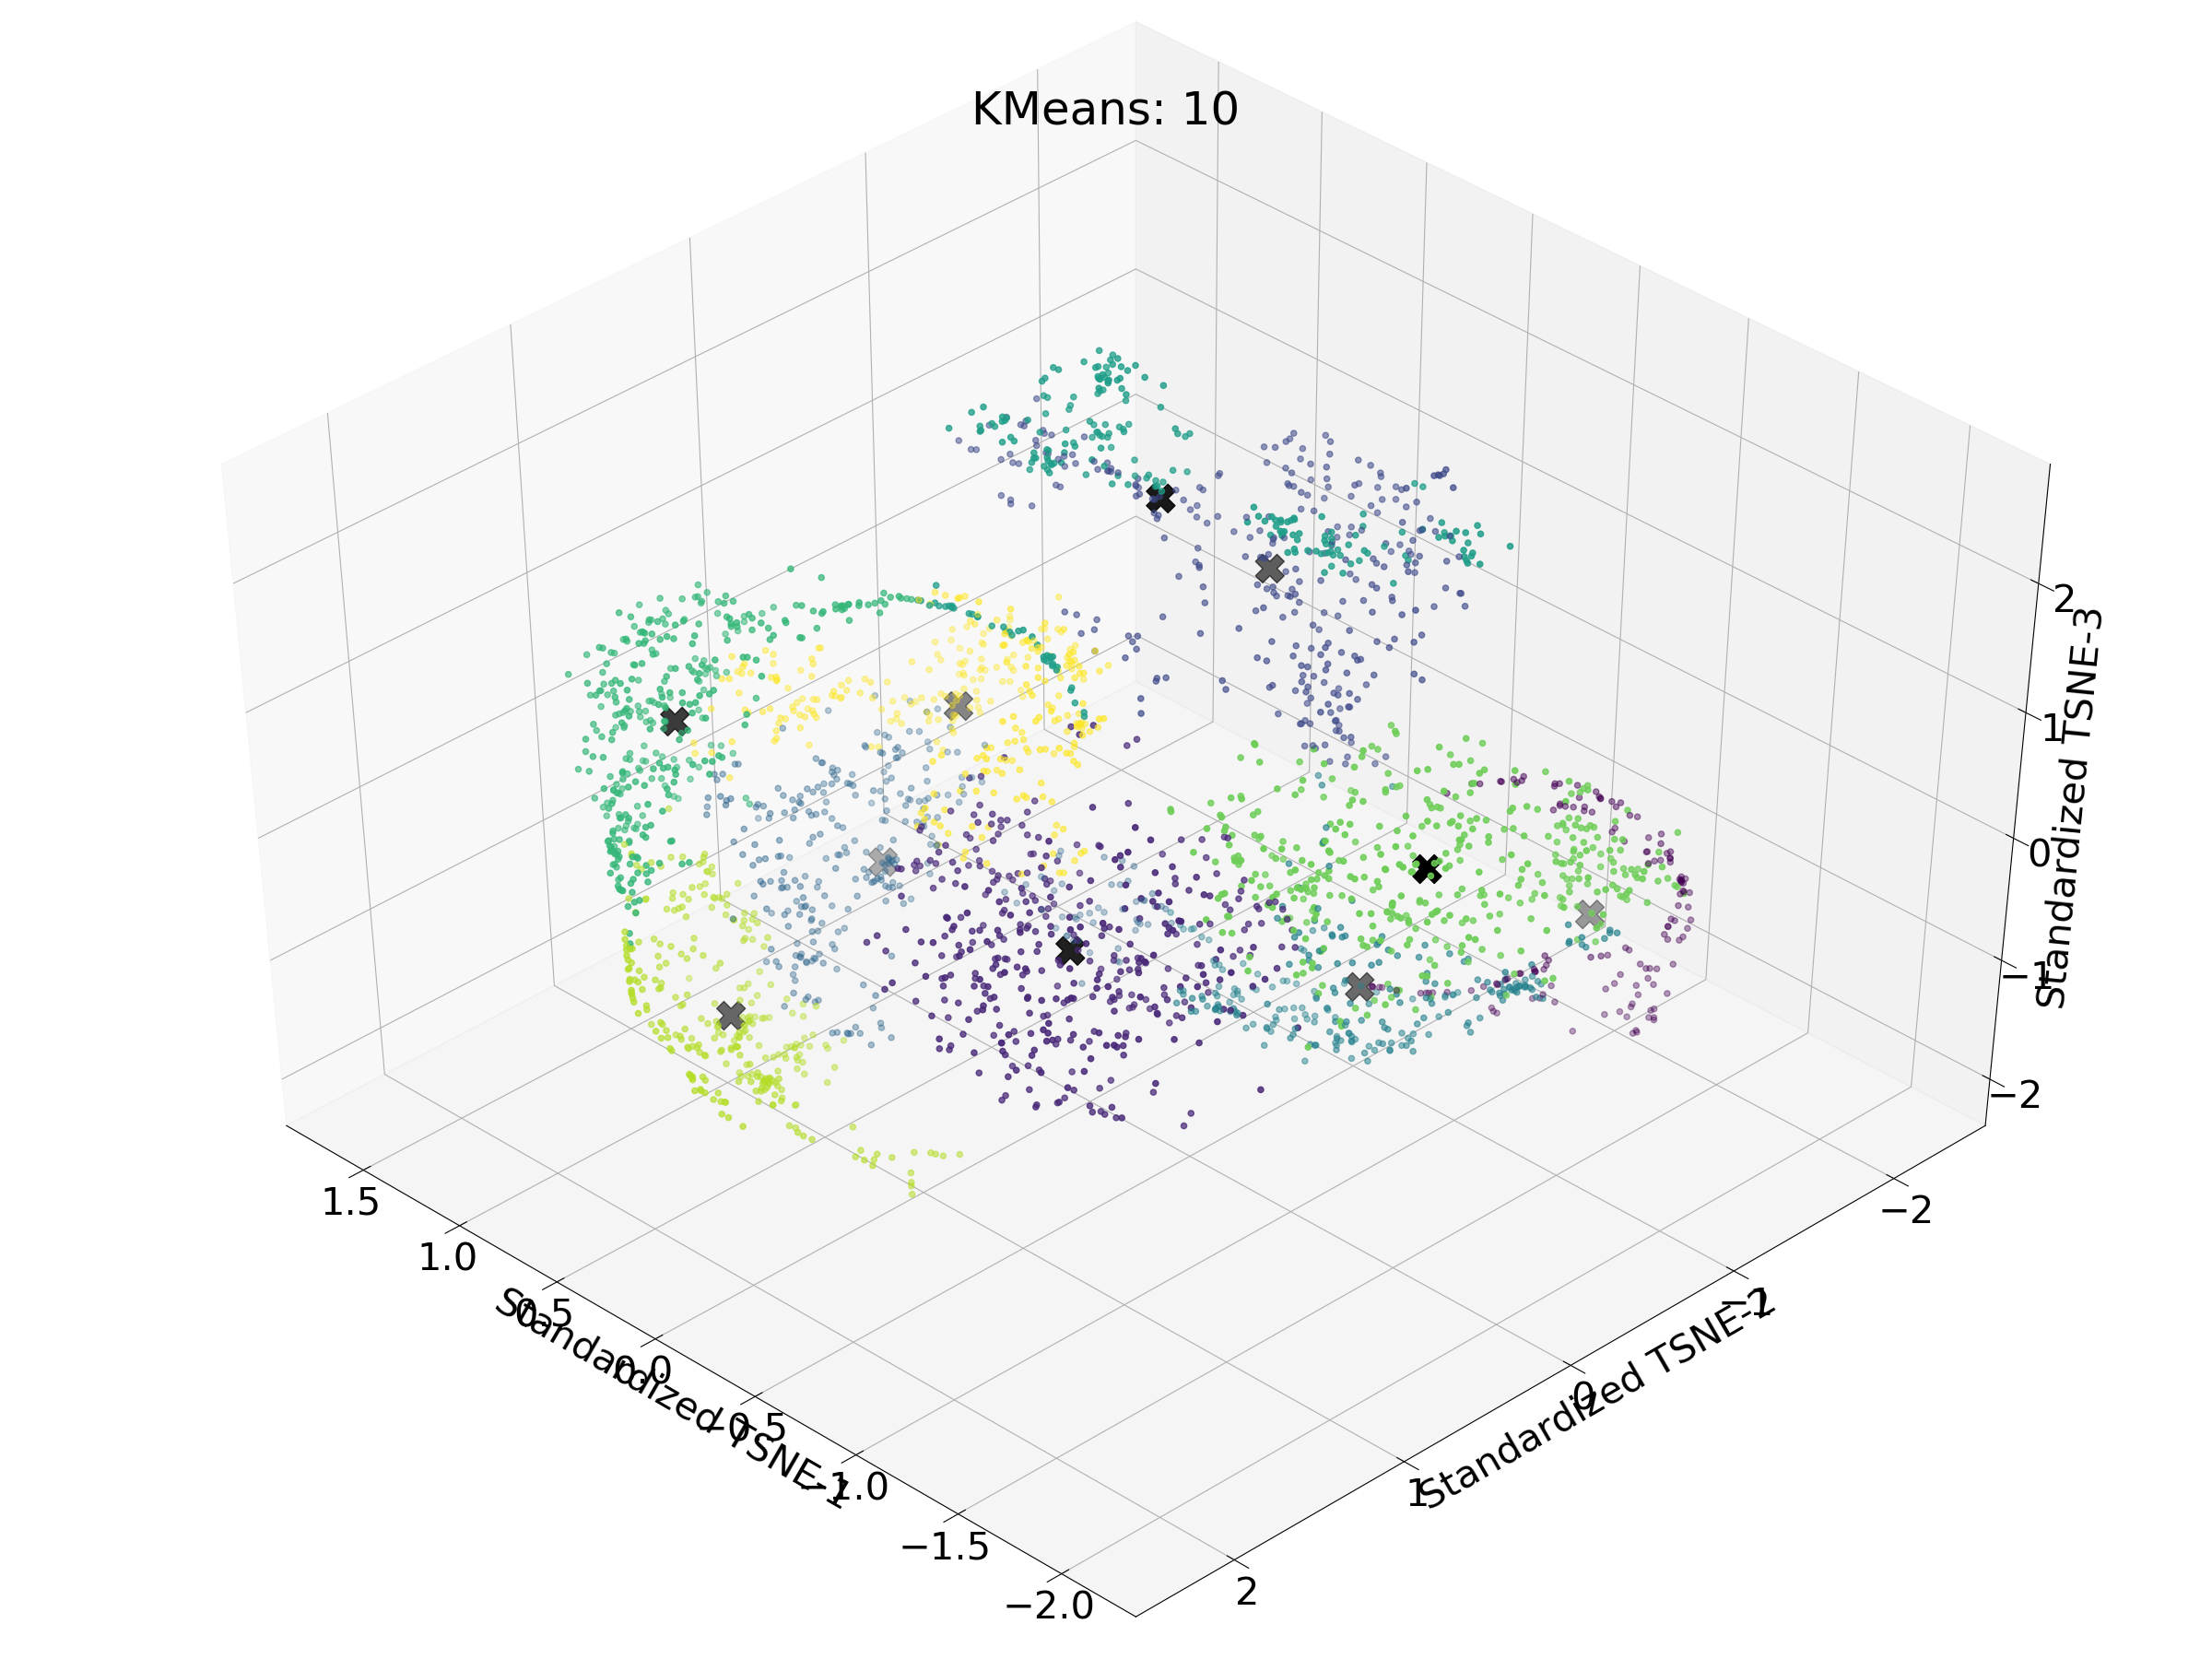
\includegraphics[height=5cm]{figures/KMeans/4.png}
                        \\
                        
                        \mbox{(c) NS\_SW3} & \mbox{(d) NS\_SW4} \\
                    \end{array}$
                \end{center}
                \caption{Results of KMeans Algorithm}
                \label{fig:kmeans}
            \end{figure}
        
            \begin{table}[h!]
                \centering
                \caption{Table of URL of 3D TSNE}
                \label{tb:cluster}
                \begin{tabular}{c c}
                    Sample & URL \\ \hline
                    NS\_SW1 & \url{https://fumire.moe/made/IKJ_Lab/cluster1.php} \\
                    NS\_SW2 & \url{https://fumire.moe/made/IKJ_Lab/cluster2.php} \\
                    NS\_SW3 & \url{https://fumire.moe/made/IKJ_Lab/cluster3.php} \\
                    NS\_SW4 & \url{https://fumire.moe/made/IKJ_Lab/cluster4.php} \\
                \end{tabular}
            \end{table}
        
        \subsection{Heatmap of Marker Gene}
            I drew a heatmap plots of marker gene. Marker gene is selected in reference. \cite{ref:sperm}
            \subsubsection{12 Genes}
                The heatmap plots with 12 genes are in figure \ref{fig:heat12genes}.
                \begin{figure}[hbp]
                    \begin{center}
                        $\begin{array}{cc}
                        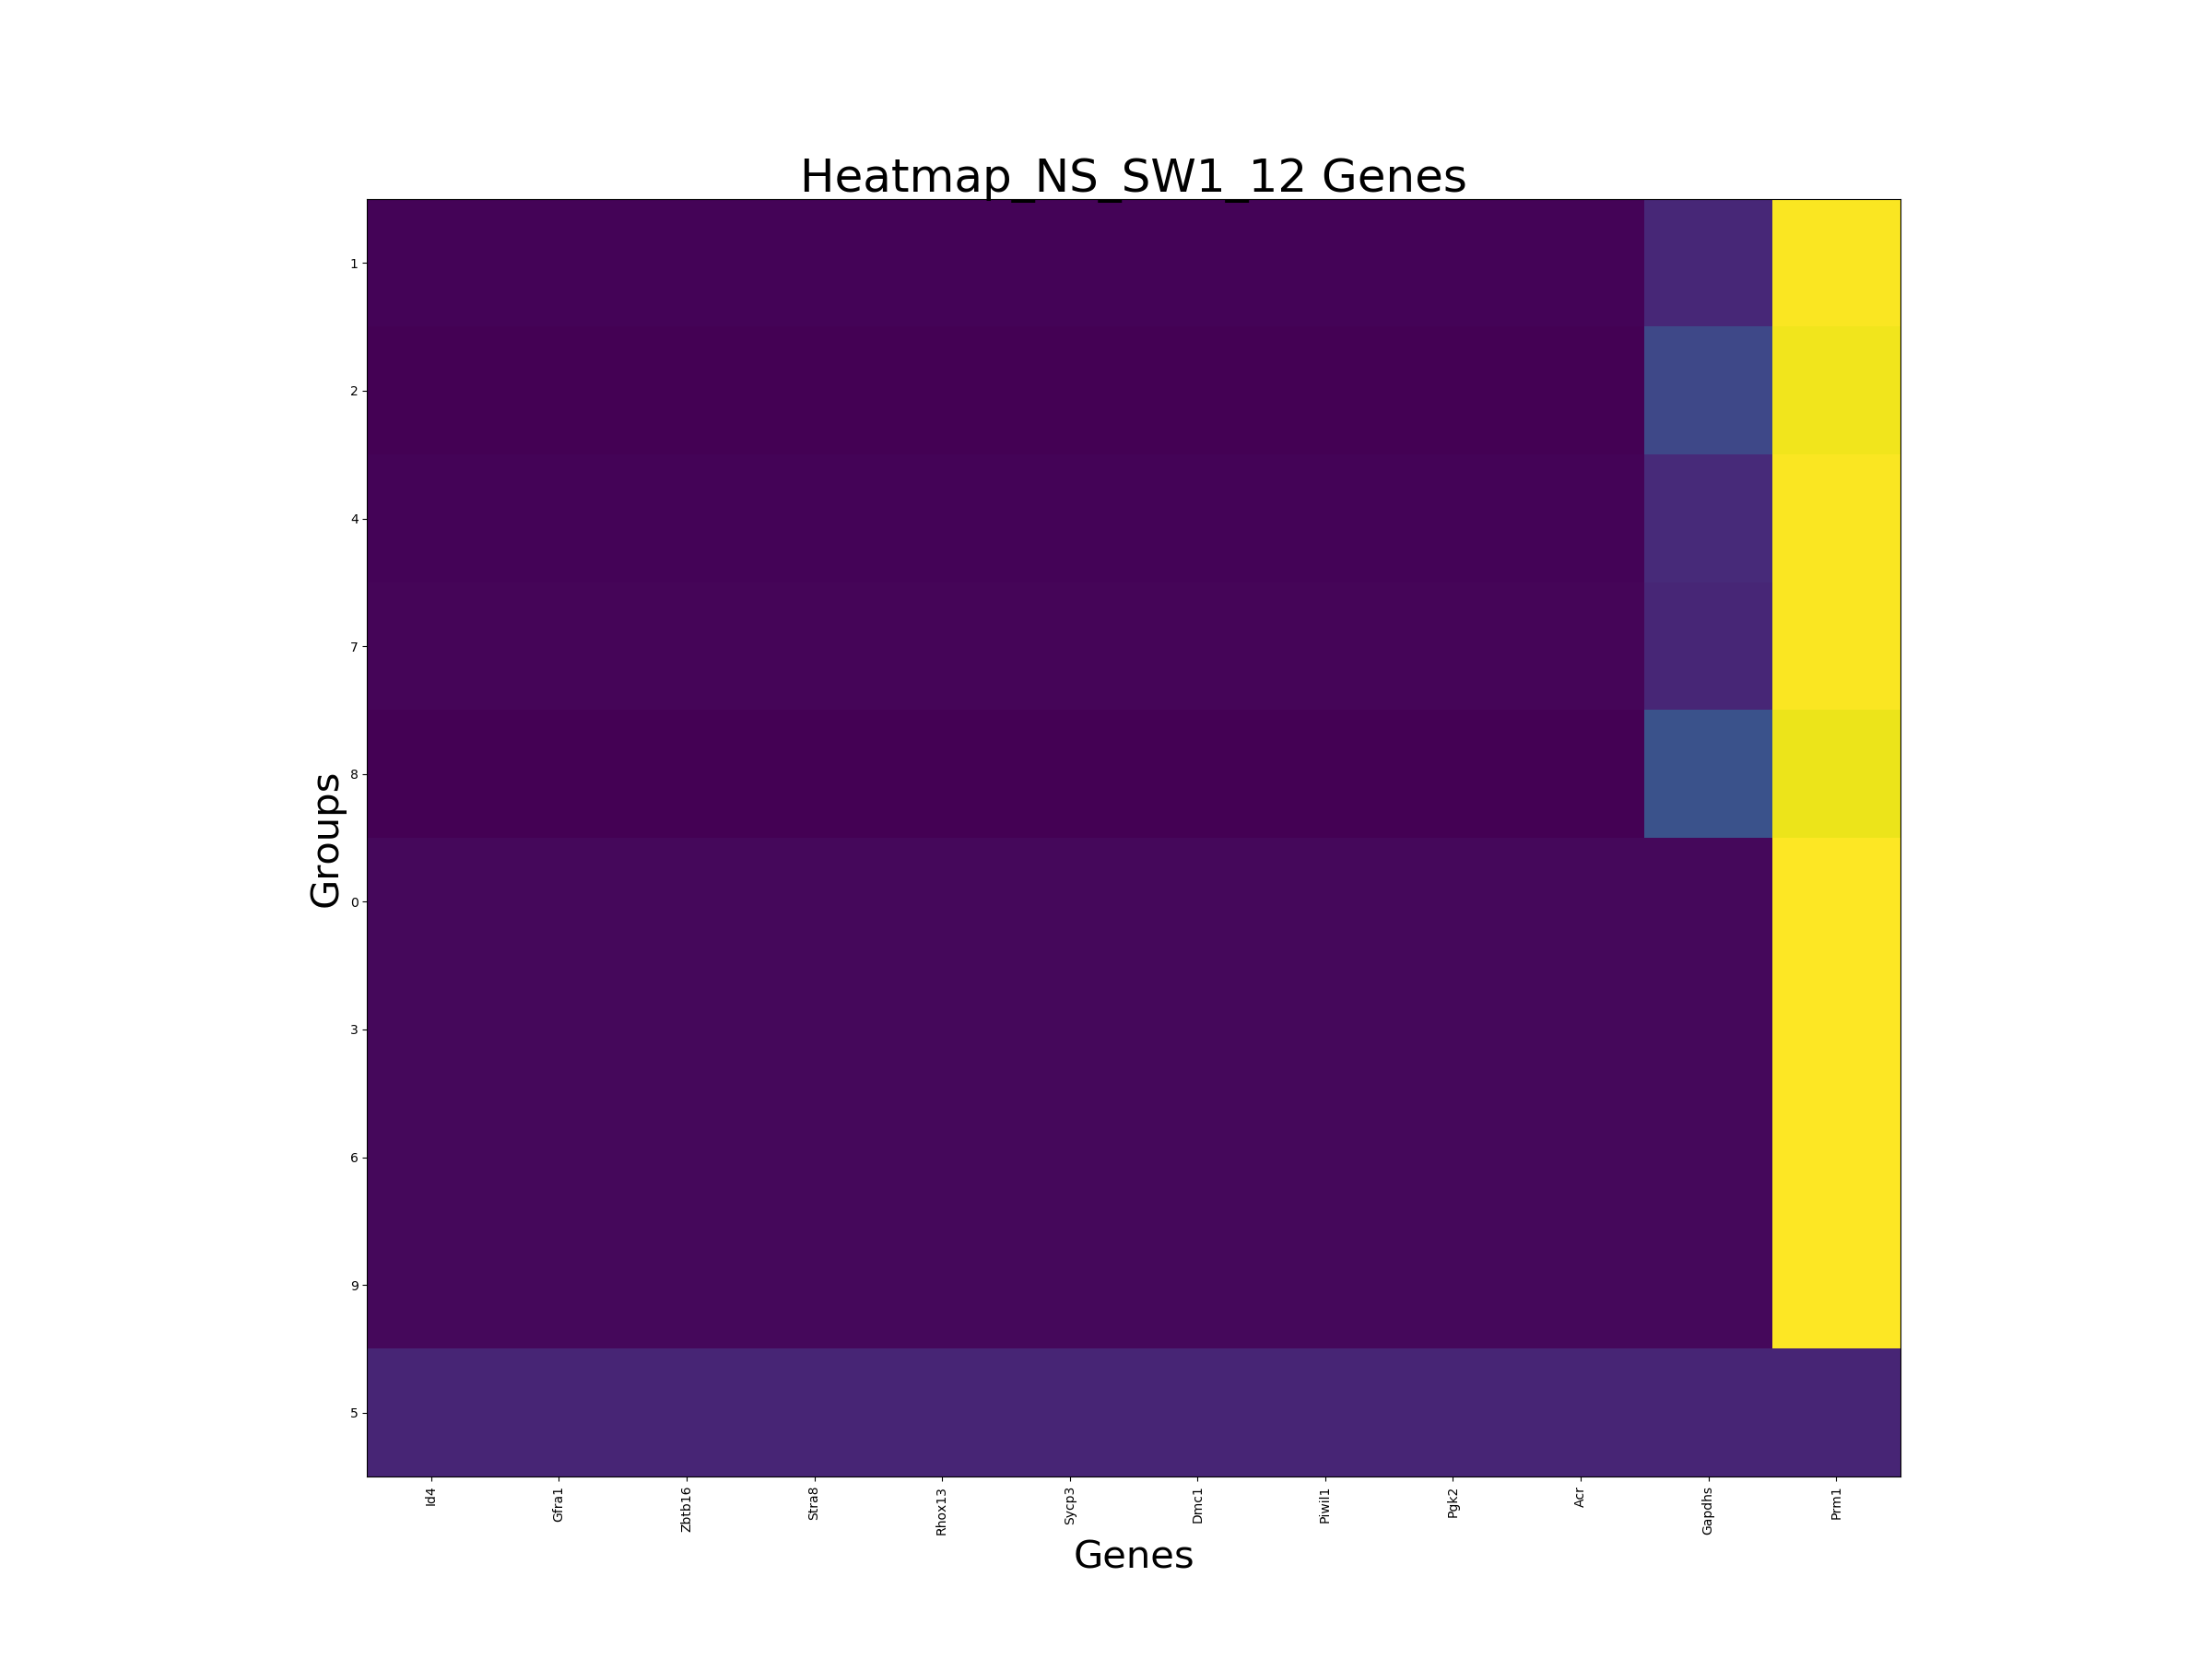
\includegraphics[height=5cm]{figures/Heatmap/12Gene/1.png}
                        &
                        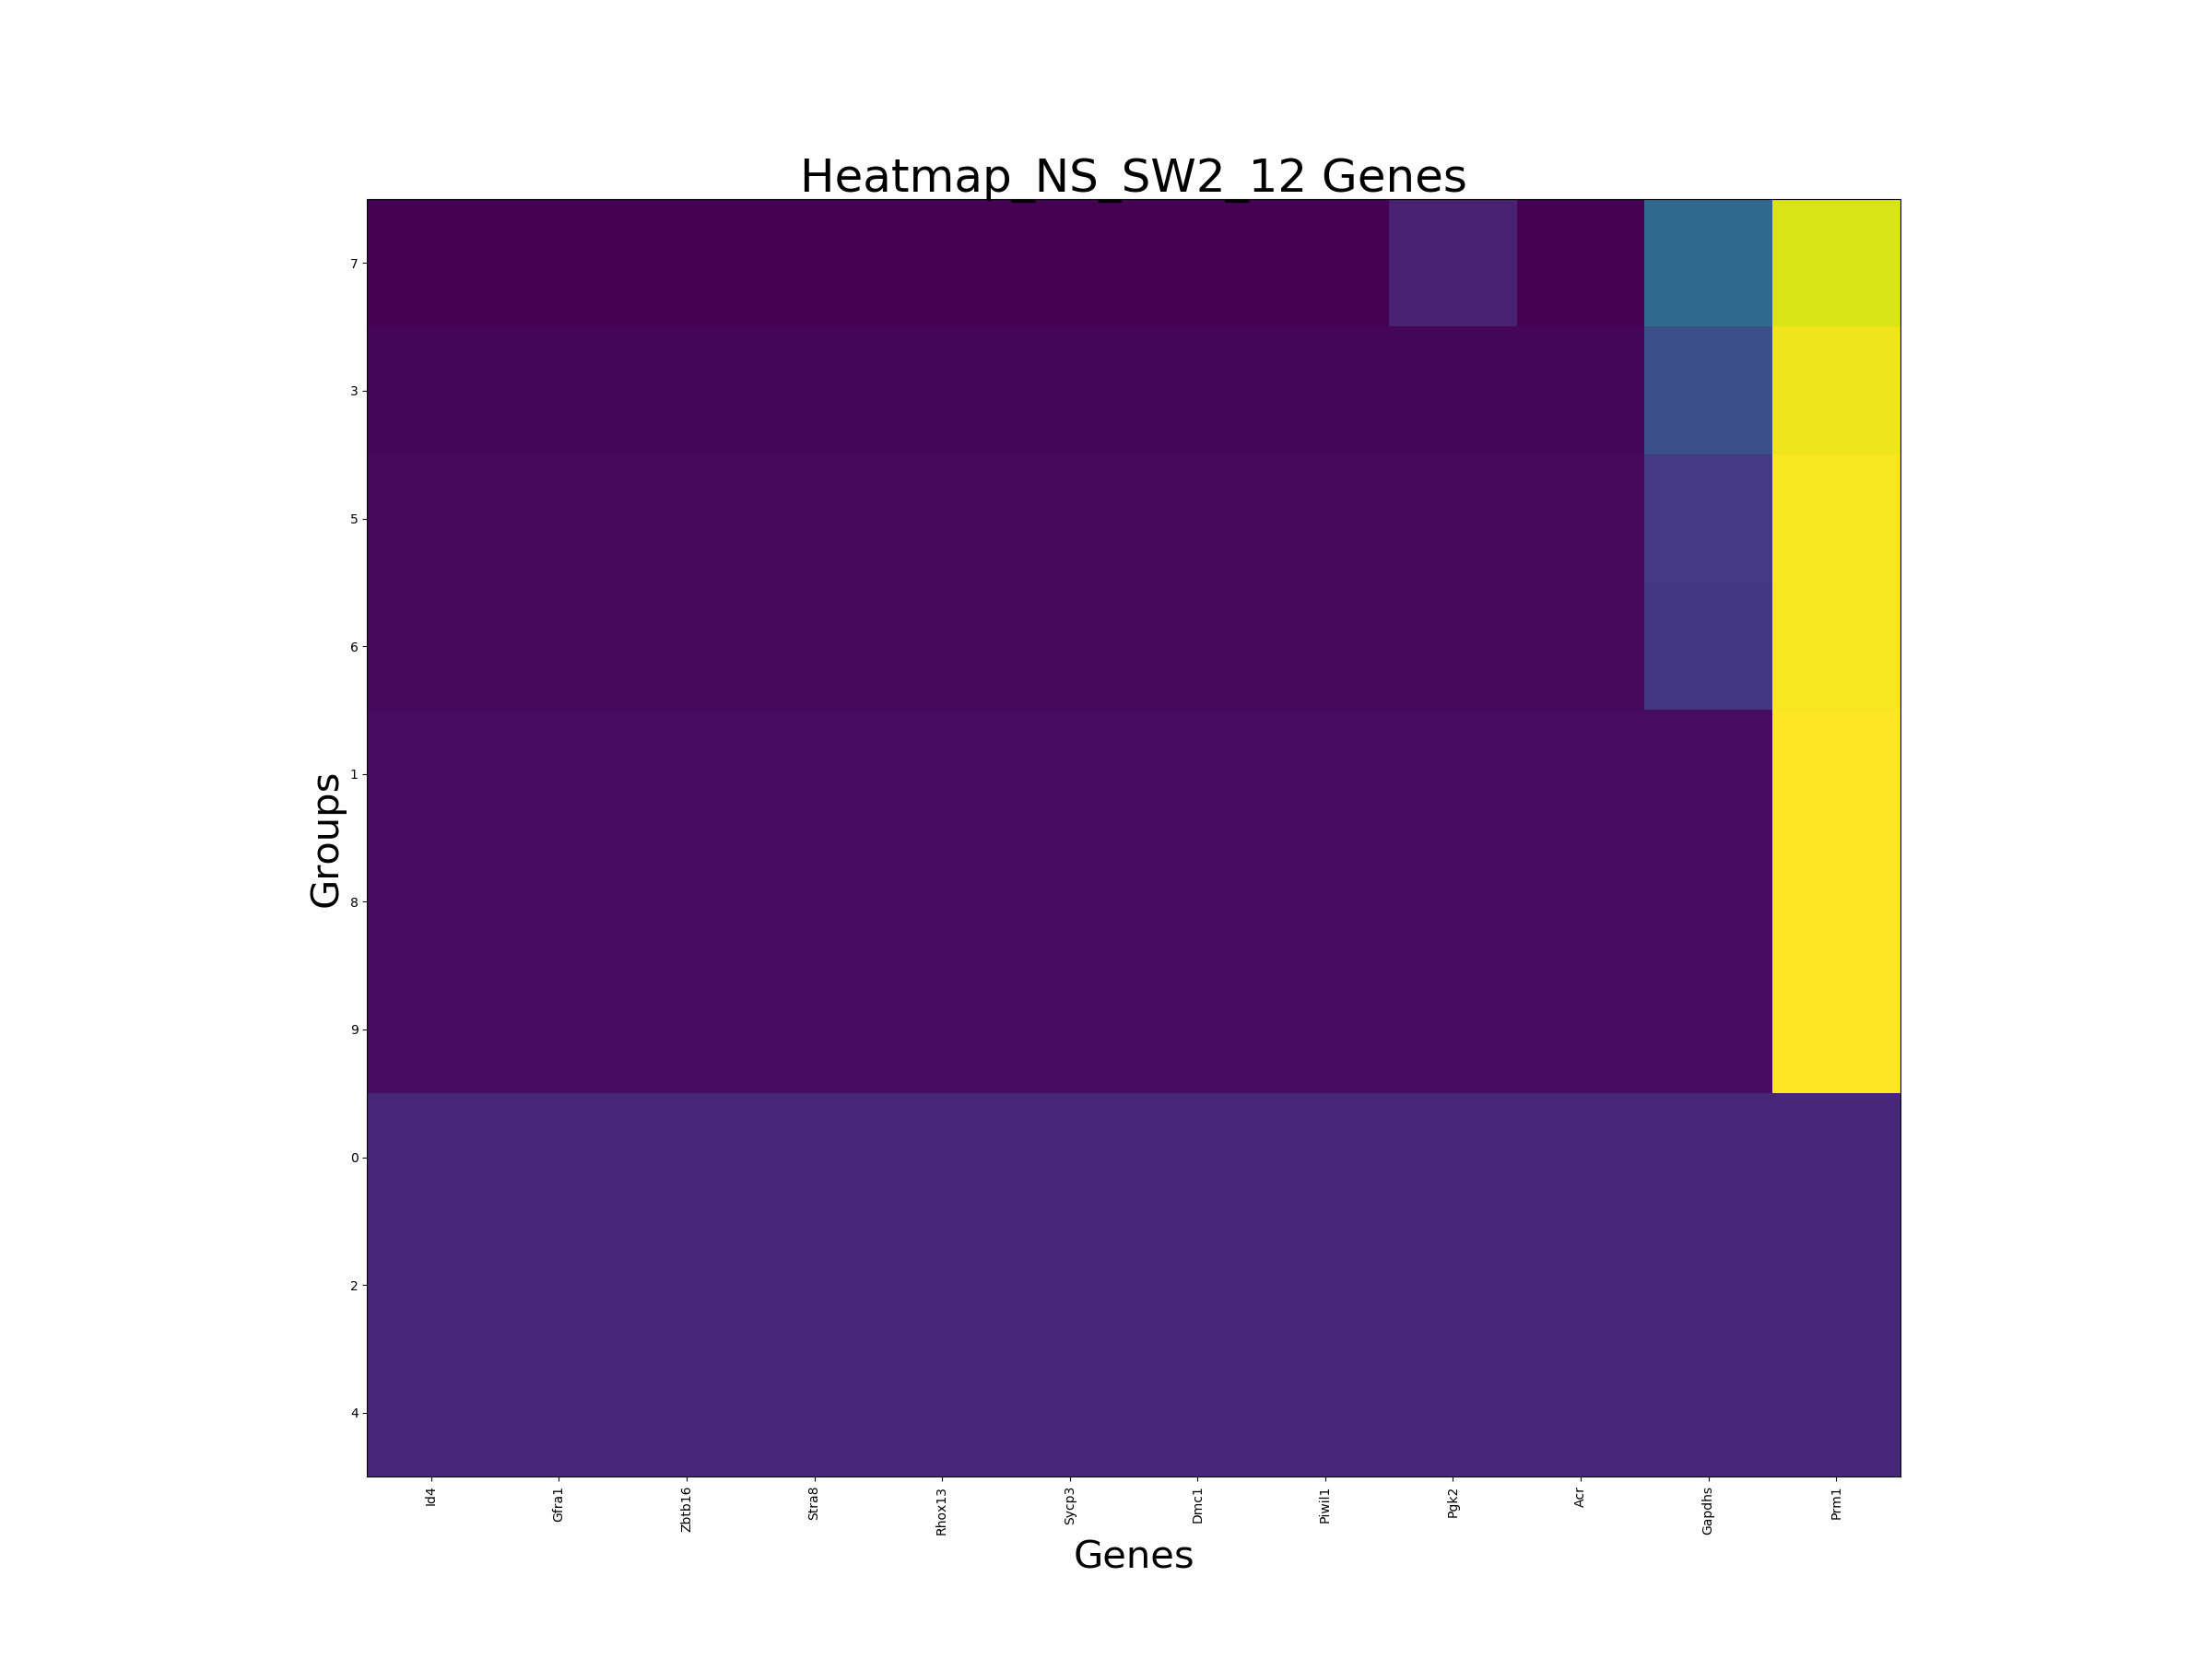
\includegraphics[height=5cm]{figures/Heatmap/12Gene/2.png}
                        \\
                        
                        \mbox{(a) NS\_SW1} & \mbox{(b) NS\_SW2} \\
                        
                        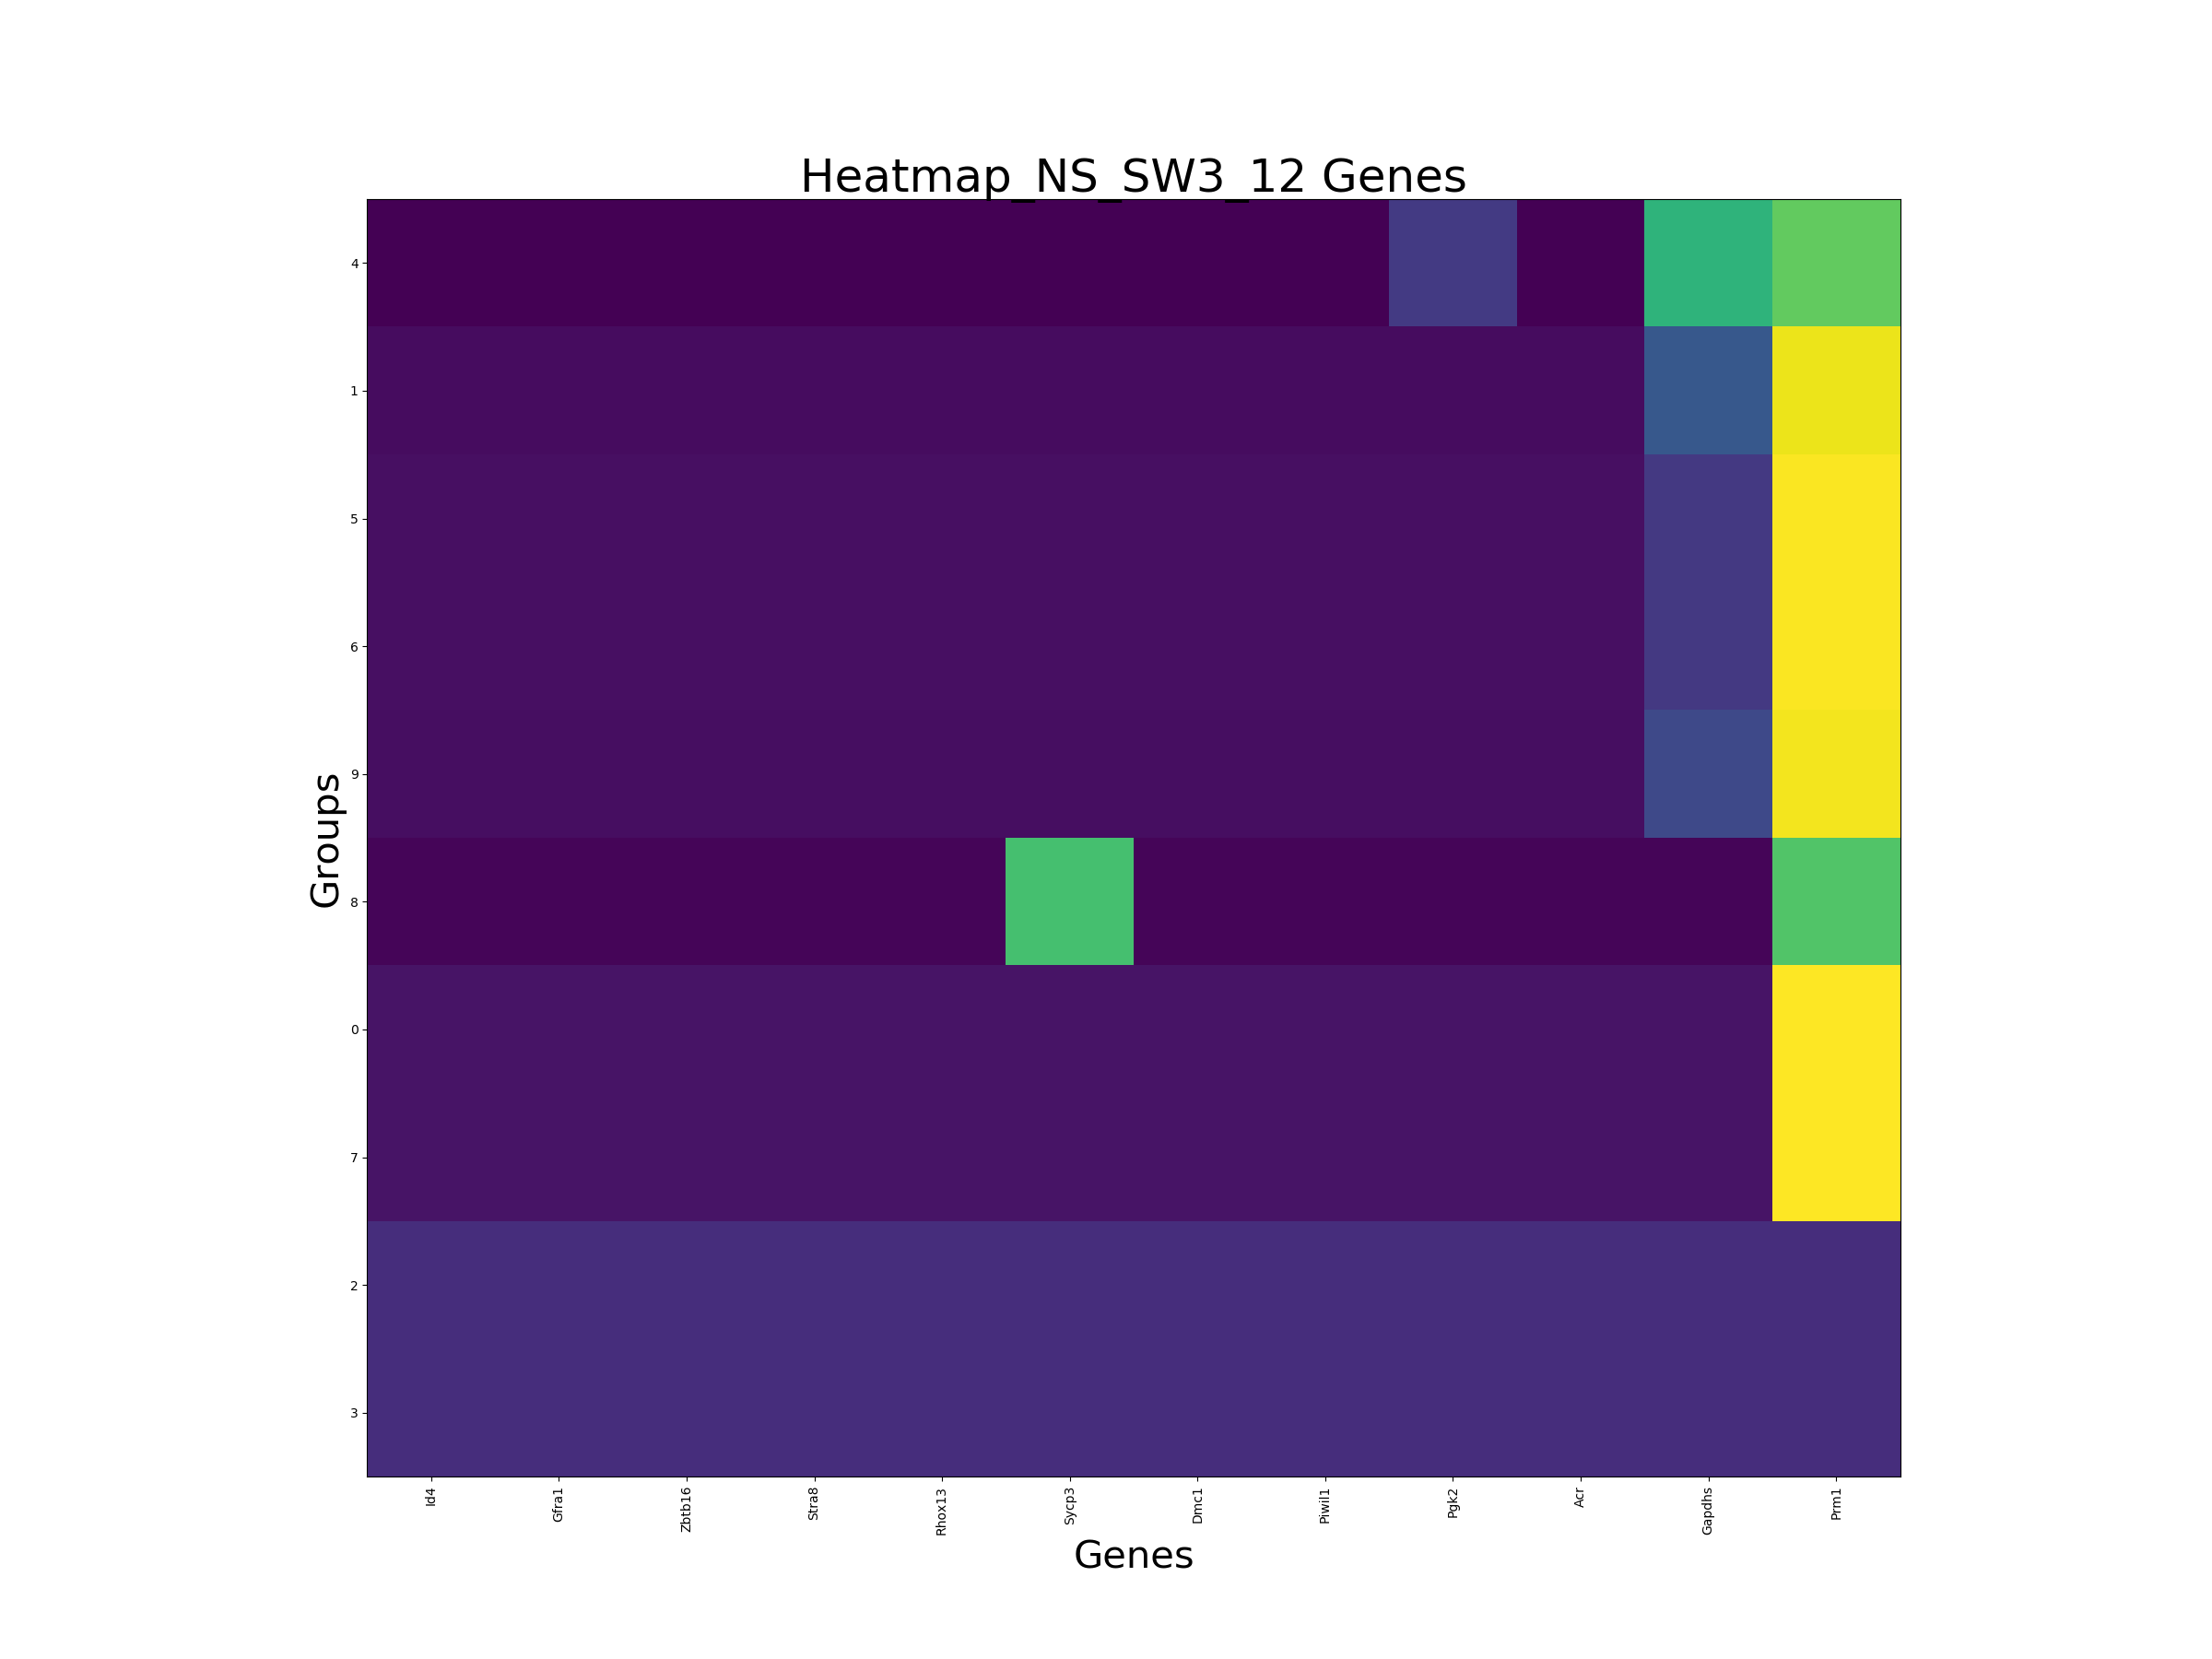
\includegraphics[height=5cm]{figures/Heatmap/12Gene/3.png}
                        &
                        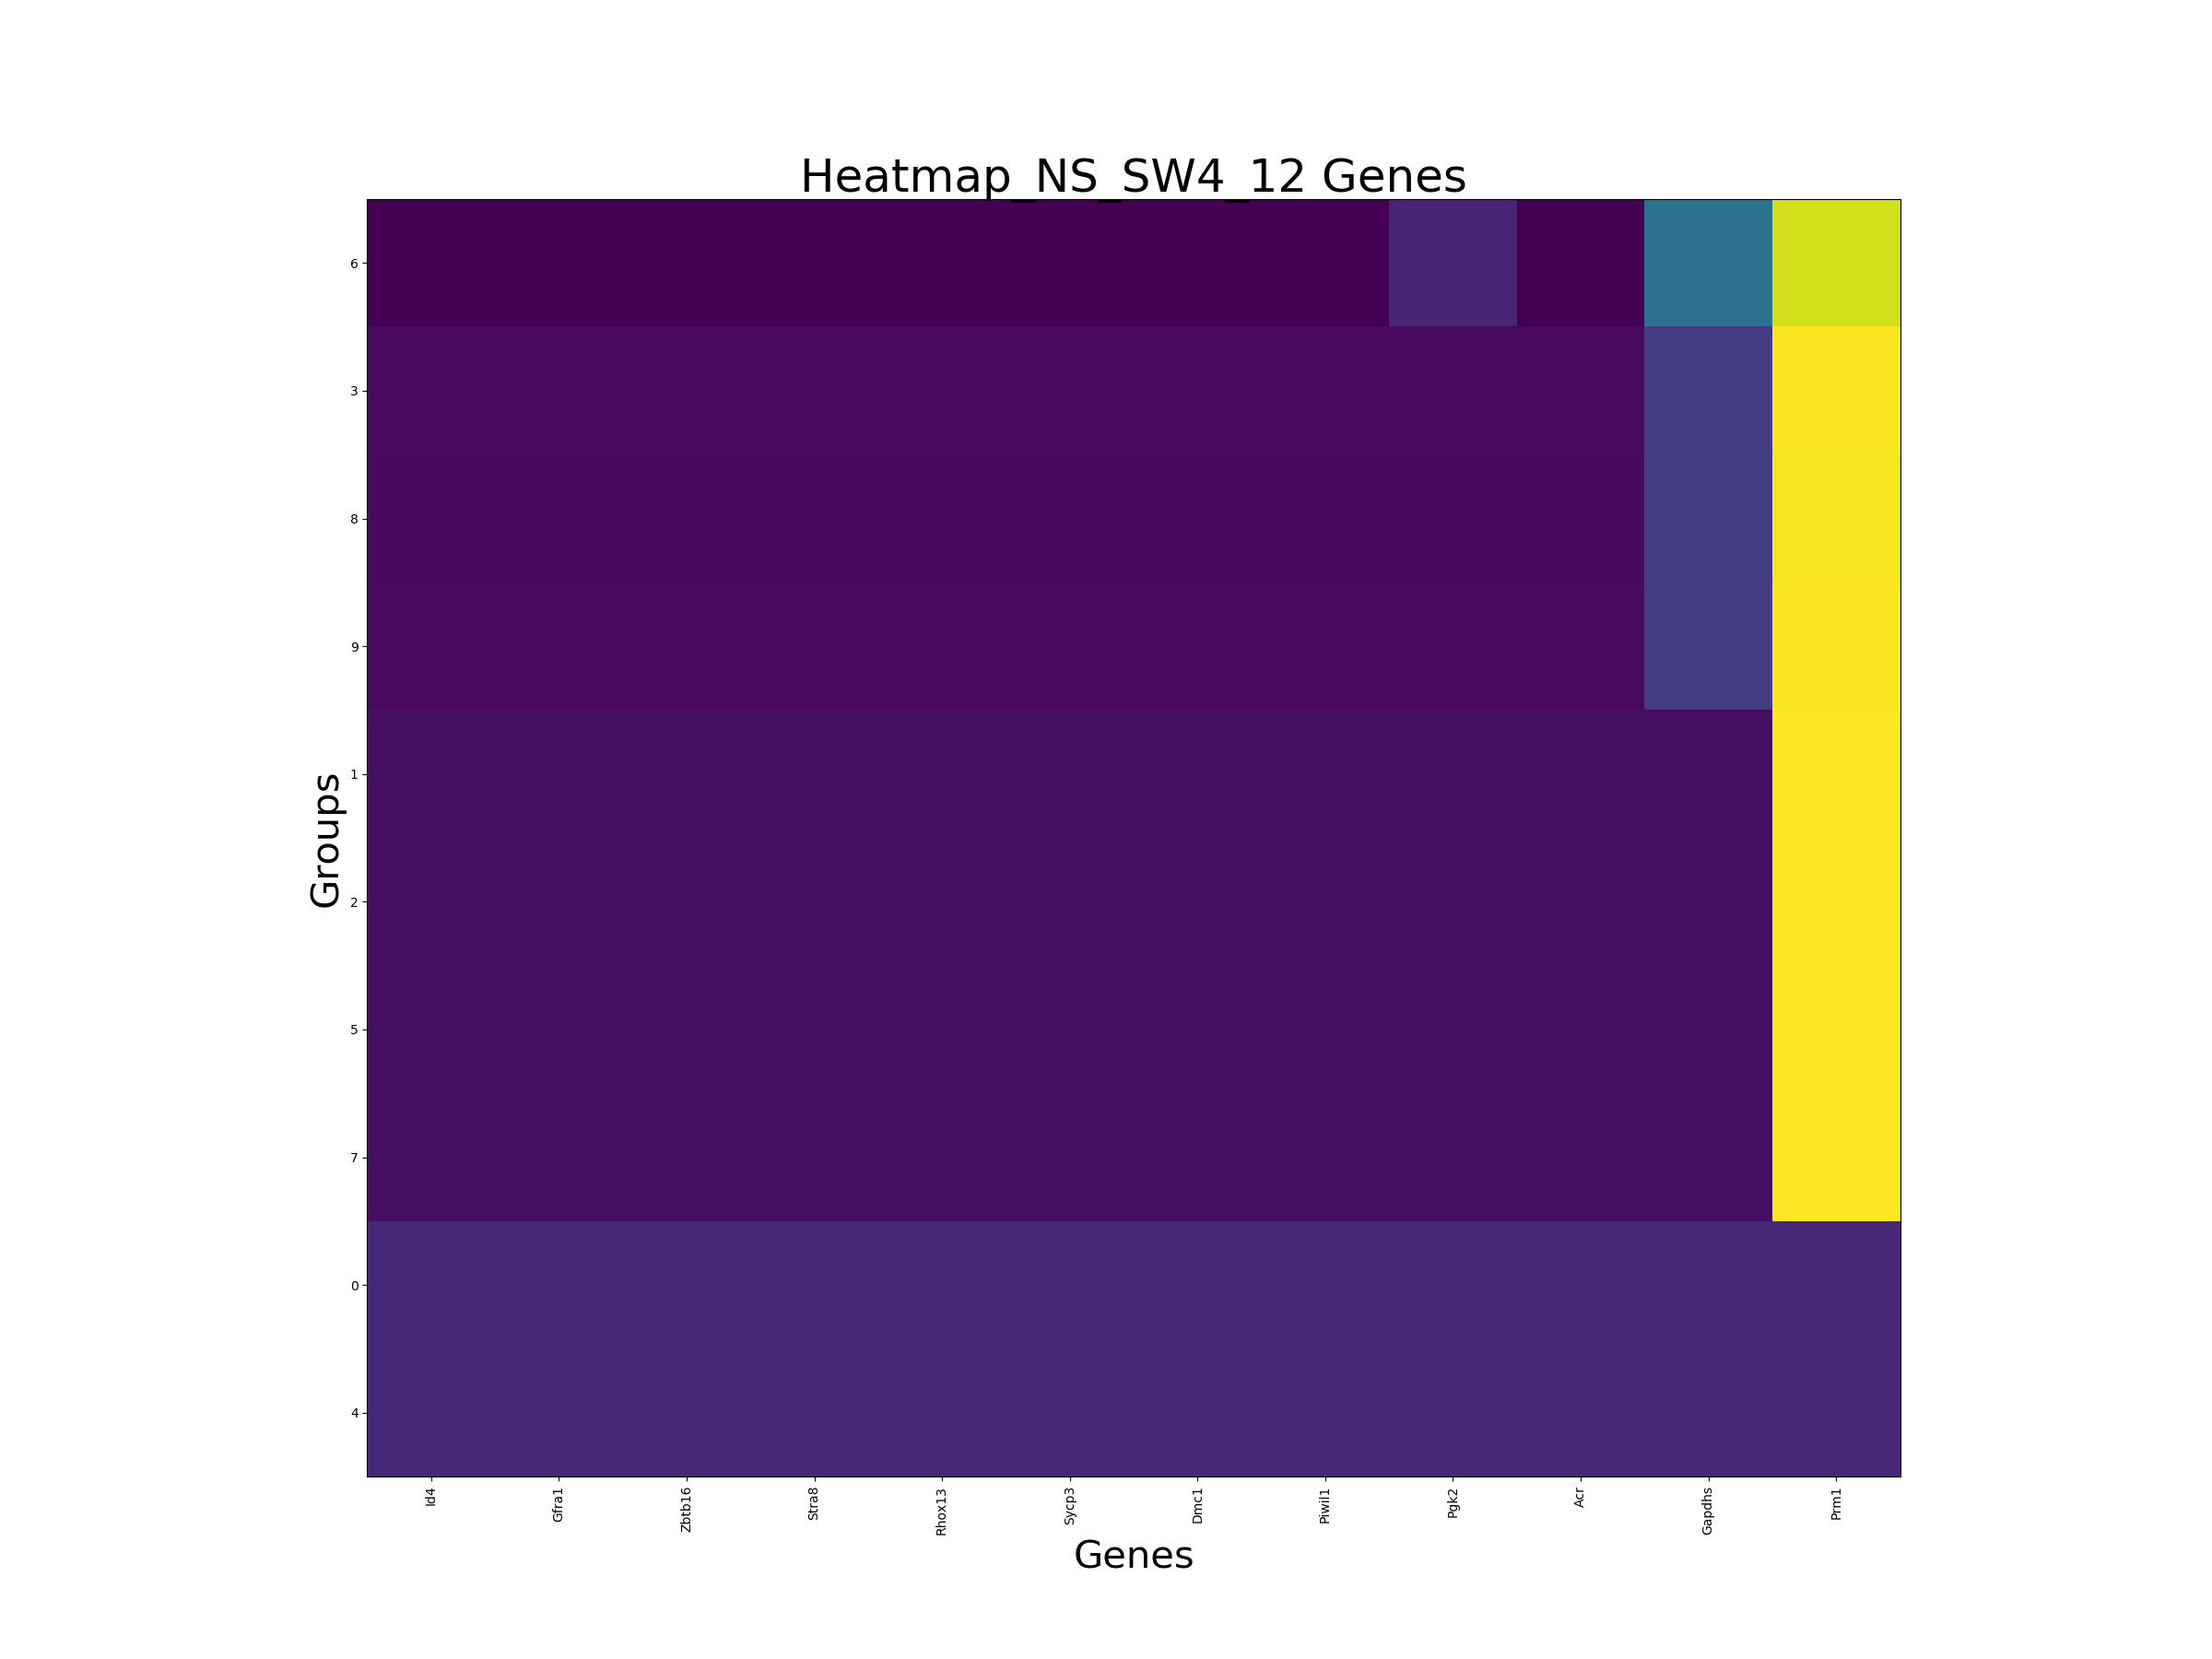
\includegraphics[height=5cm]{figures/Heatmap/12Gene/4.png}
                        \\
                        
                        \mbox{(c) NS\_SW3} & \mbox{(d) NS\_SW4} \\
                    \end{array}$
                    \end{center}
                    \caption{Heatmap Plot of 12 Marker Genes}
                    \label{fig:heat12genes}
                \end{figure}
            \subsubsection{65 Genes}
                The heatmap plots with 65 genes are in figure \ref{fig:heat65gene}. 
                \begin{figure}[hbp]
                    \begin{center}
                        $\begin{array}{cc}
                        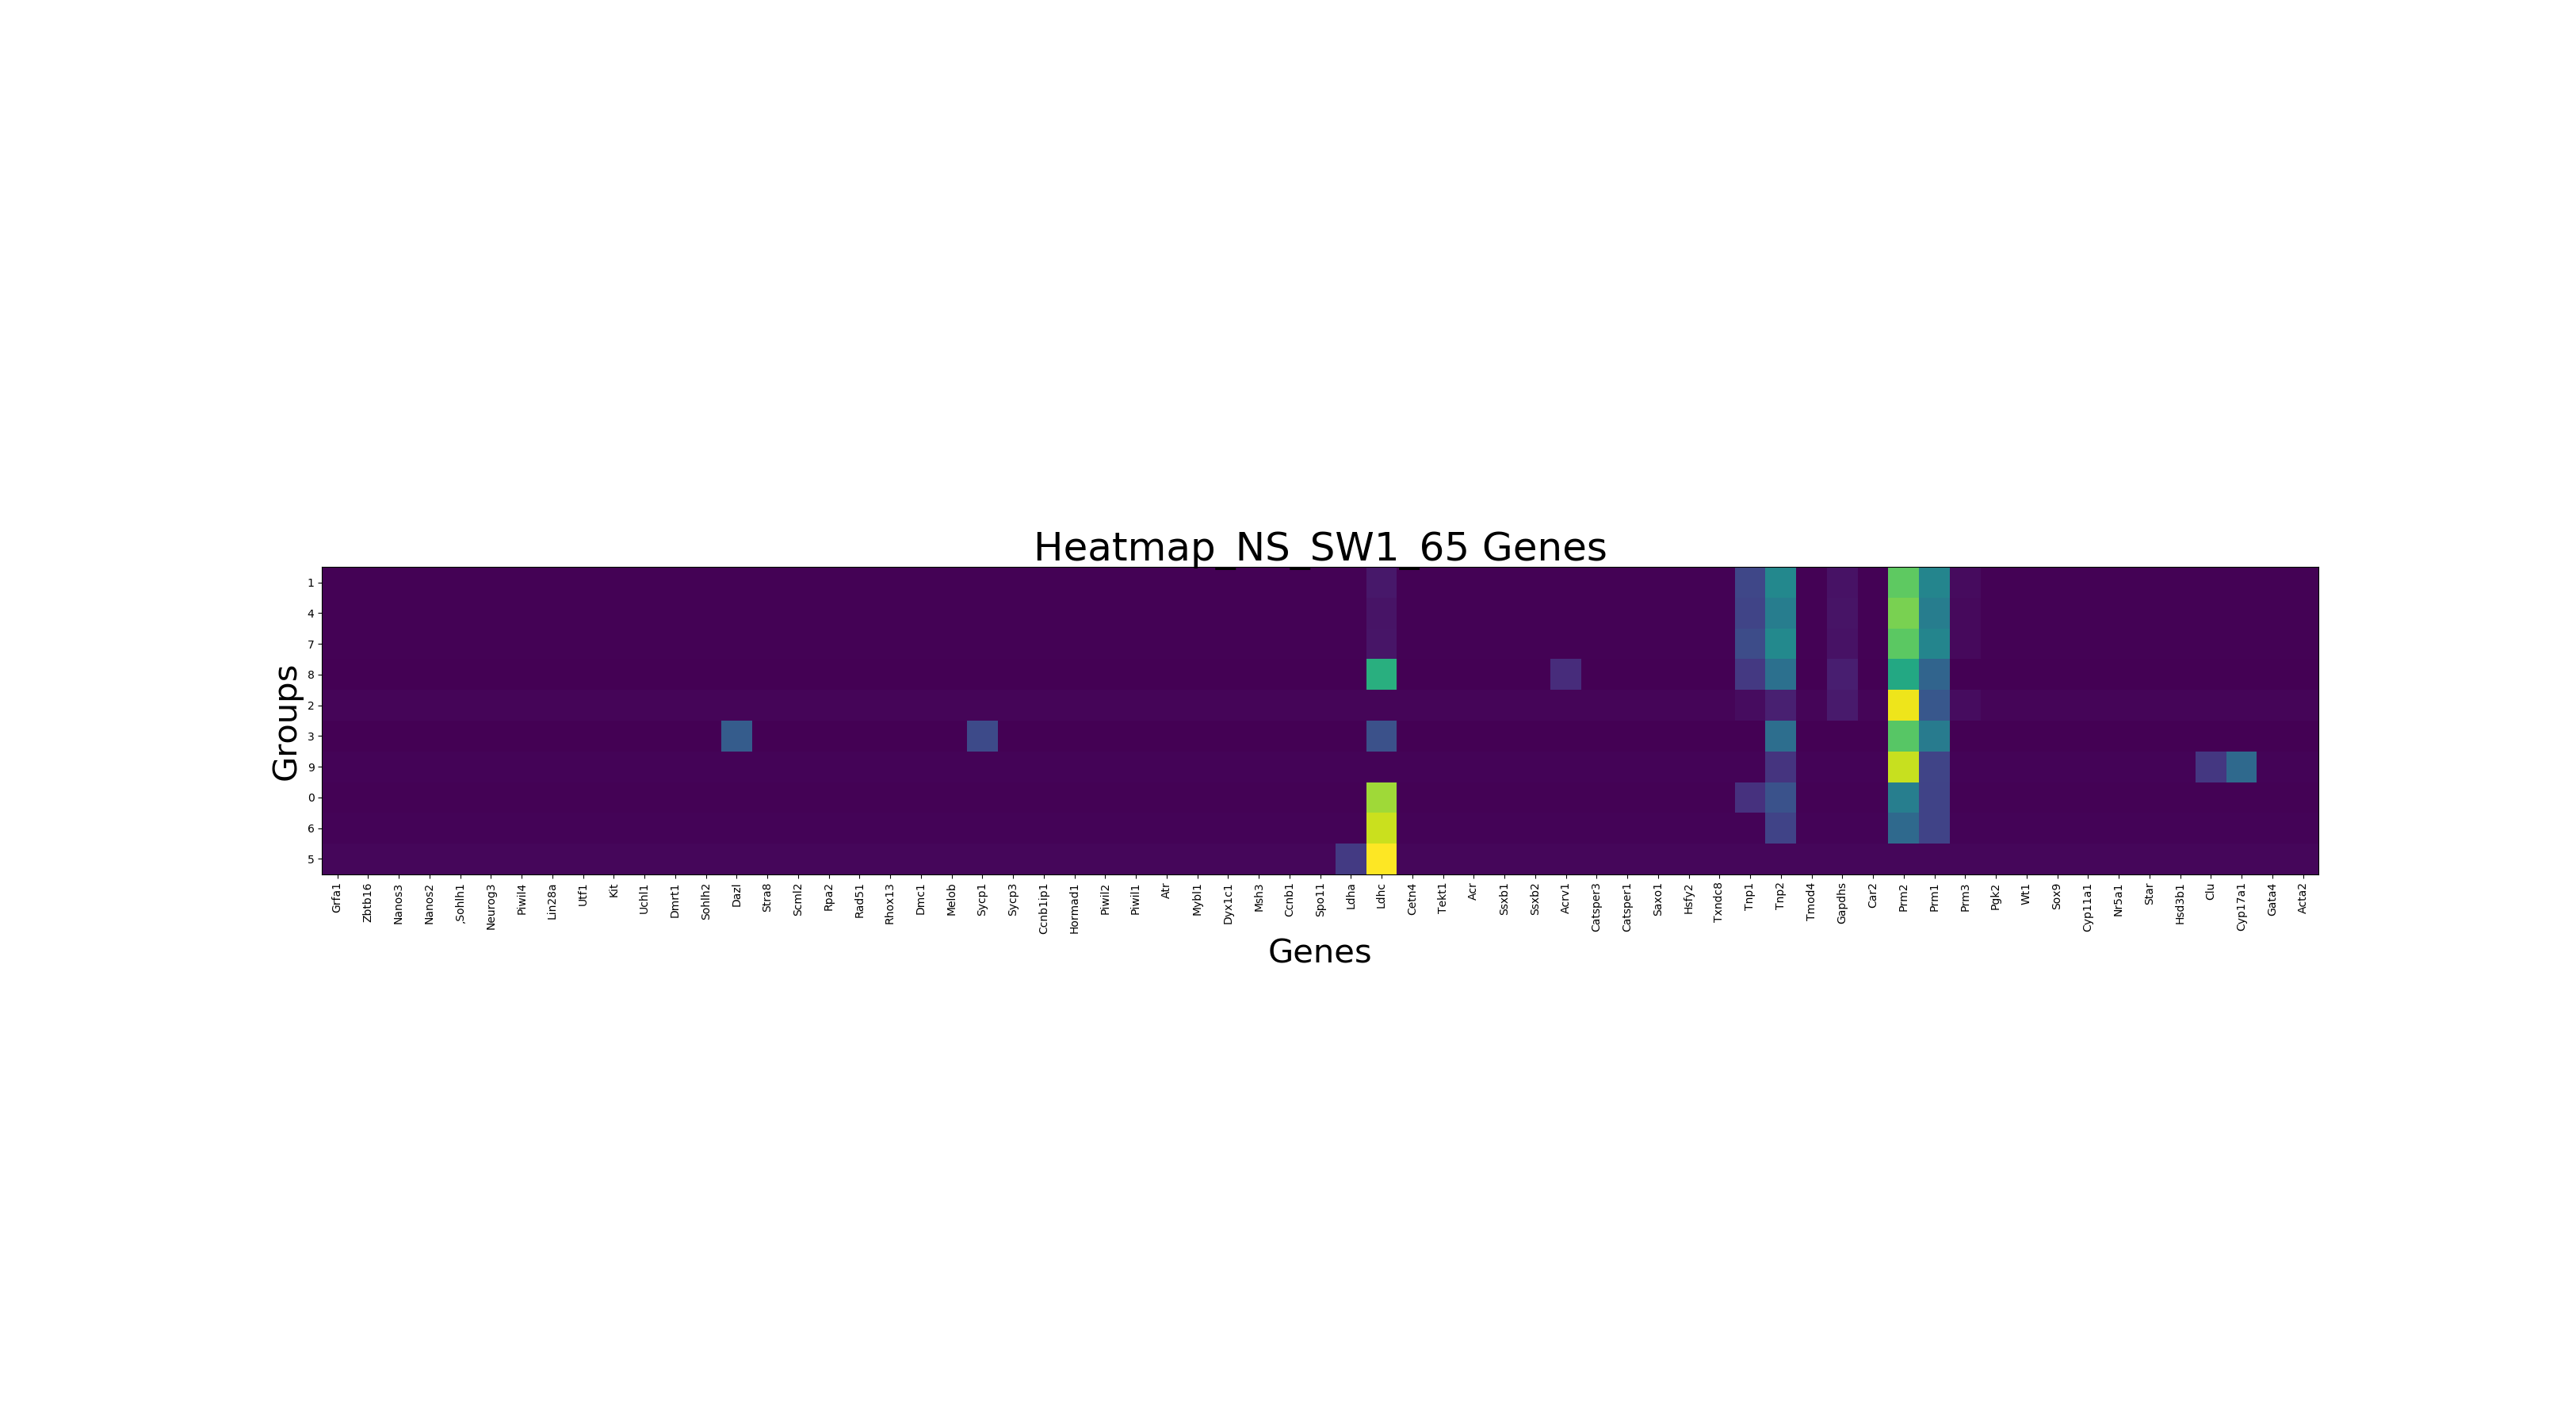
\includegraphics[width=8cm]{figures/Heatmap/65Gene/1.png}
                        &
                        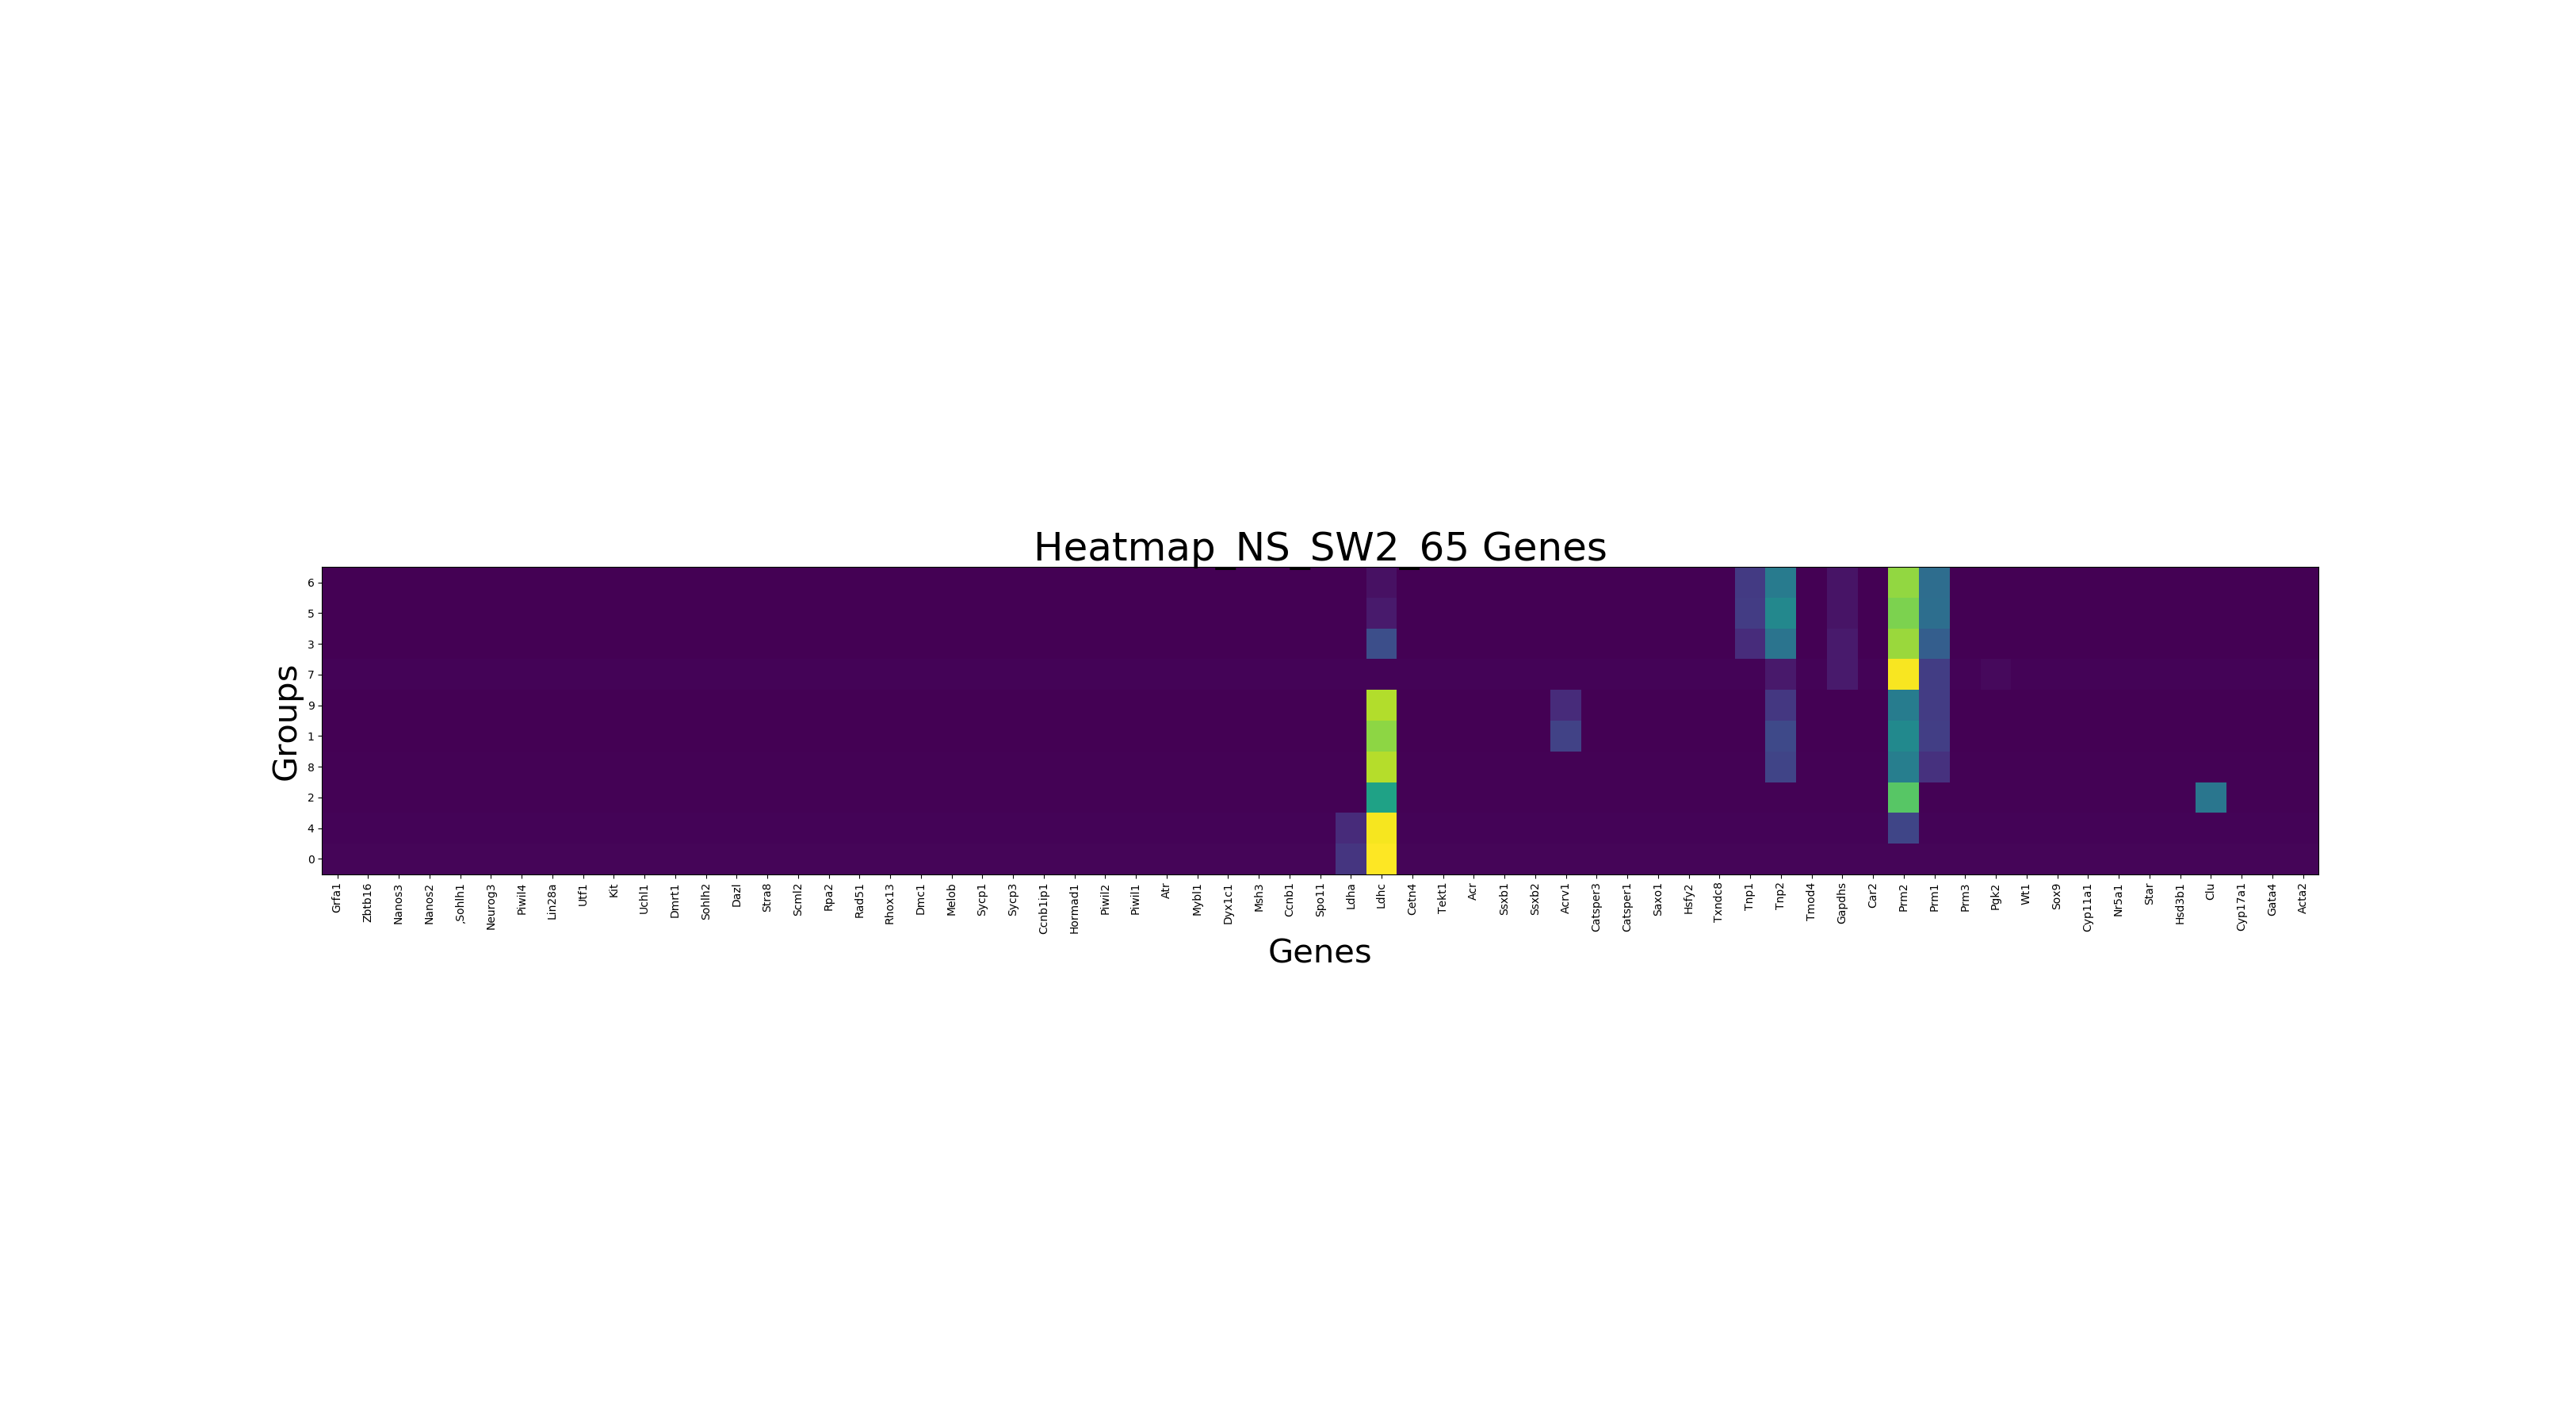
\includegraphics[width=8cm]{figures/Heatmap/65Gene/2.png}
                        \\
                        
                        \mbox{(a) NS\_SW1} & \mbox{(b) NS\_SW2} \\
                        
                        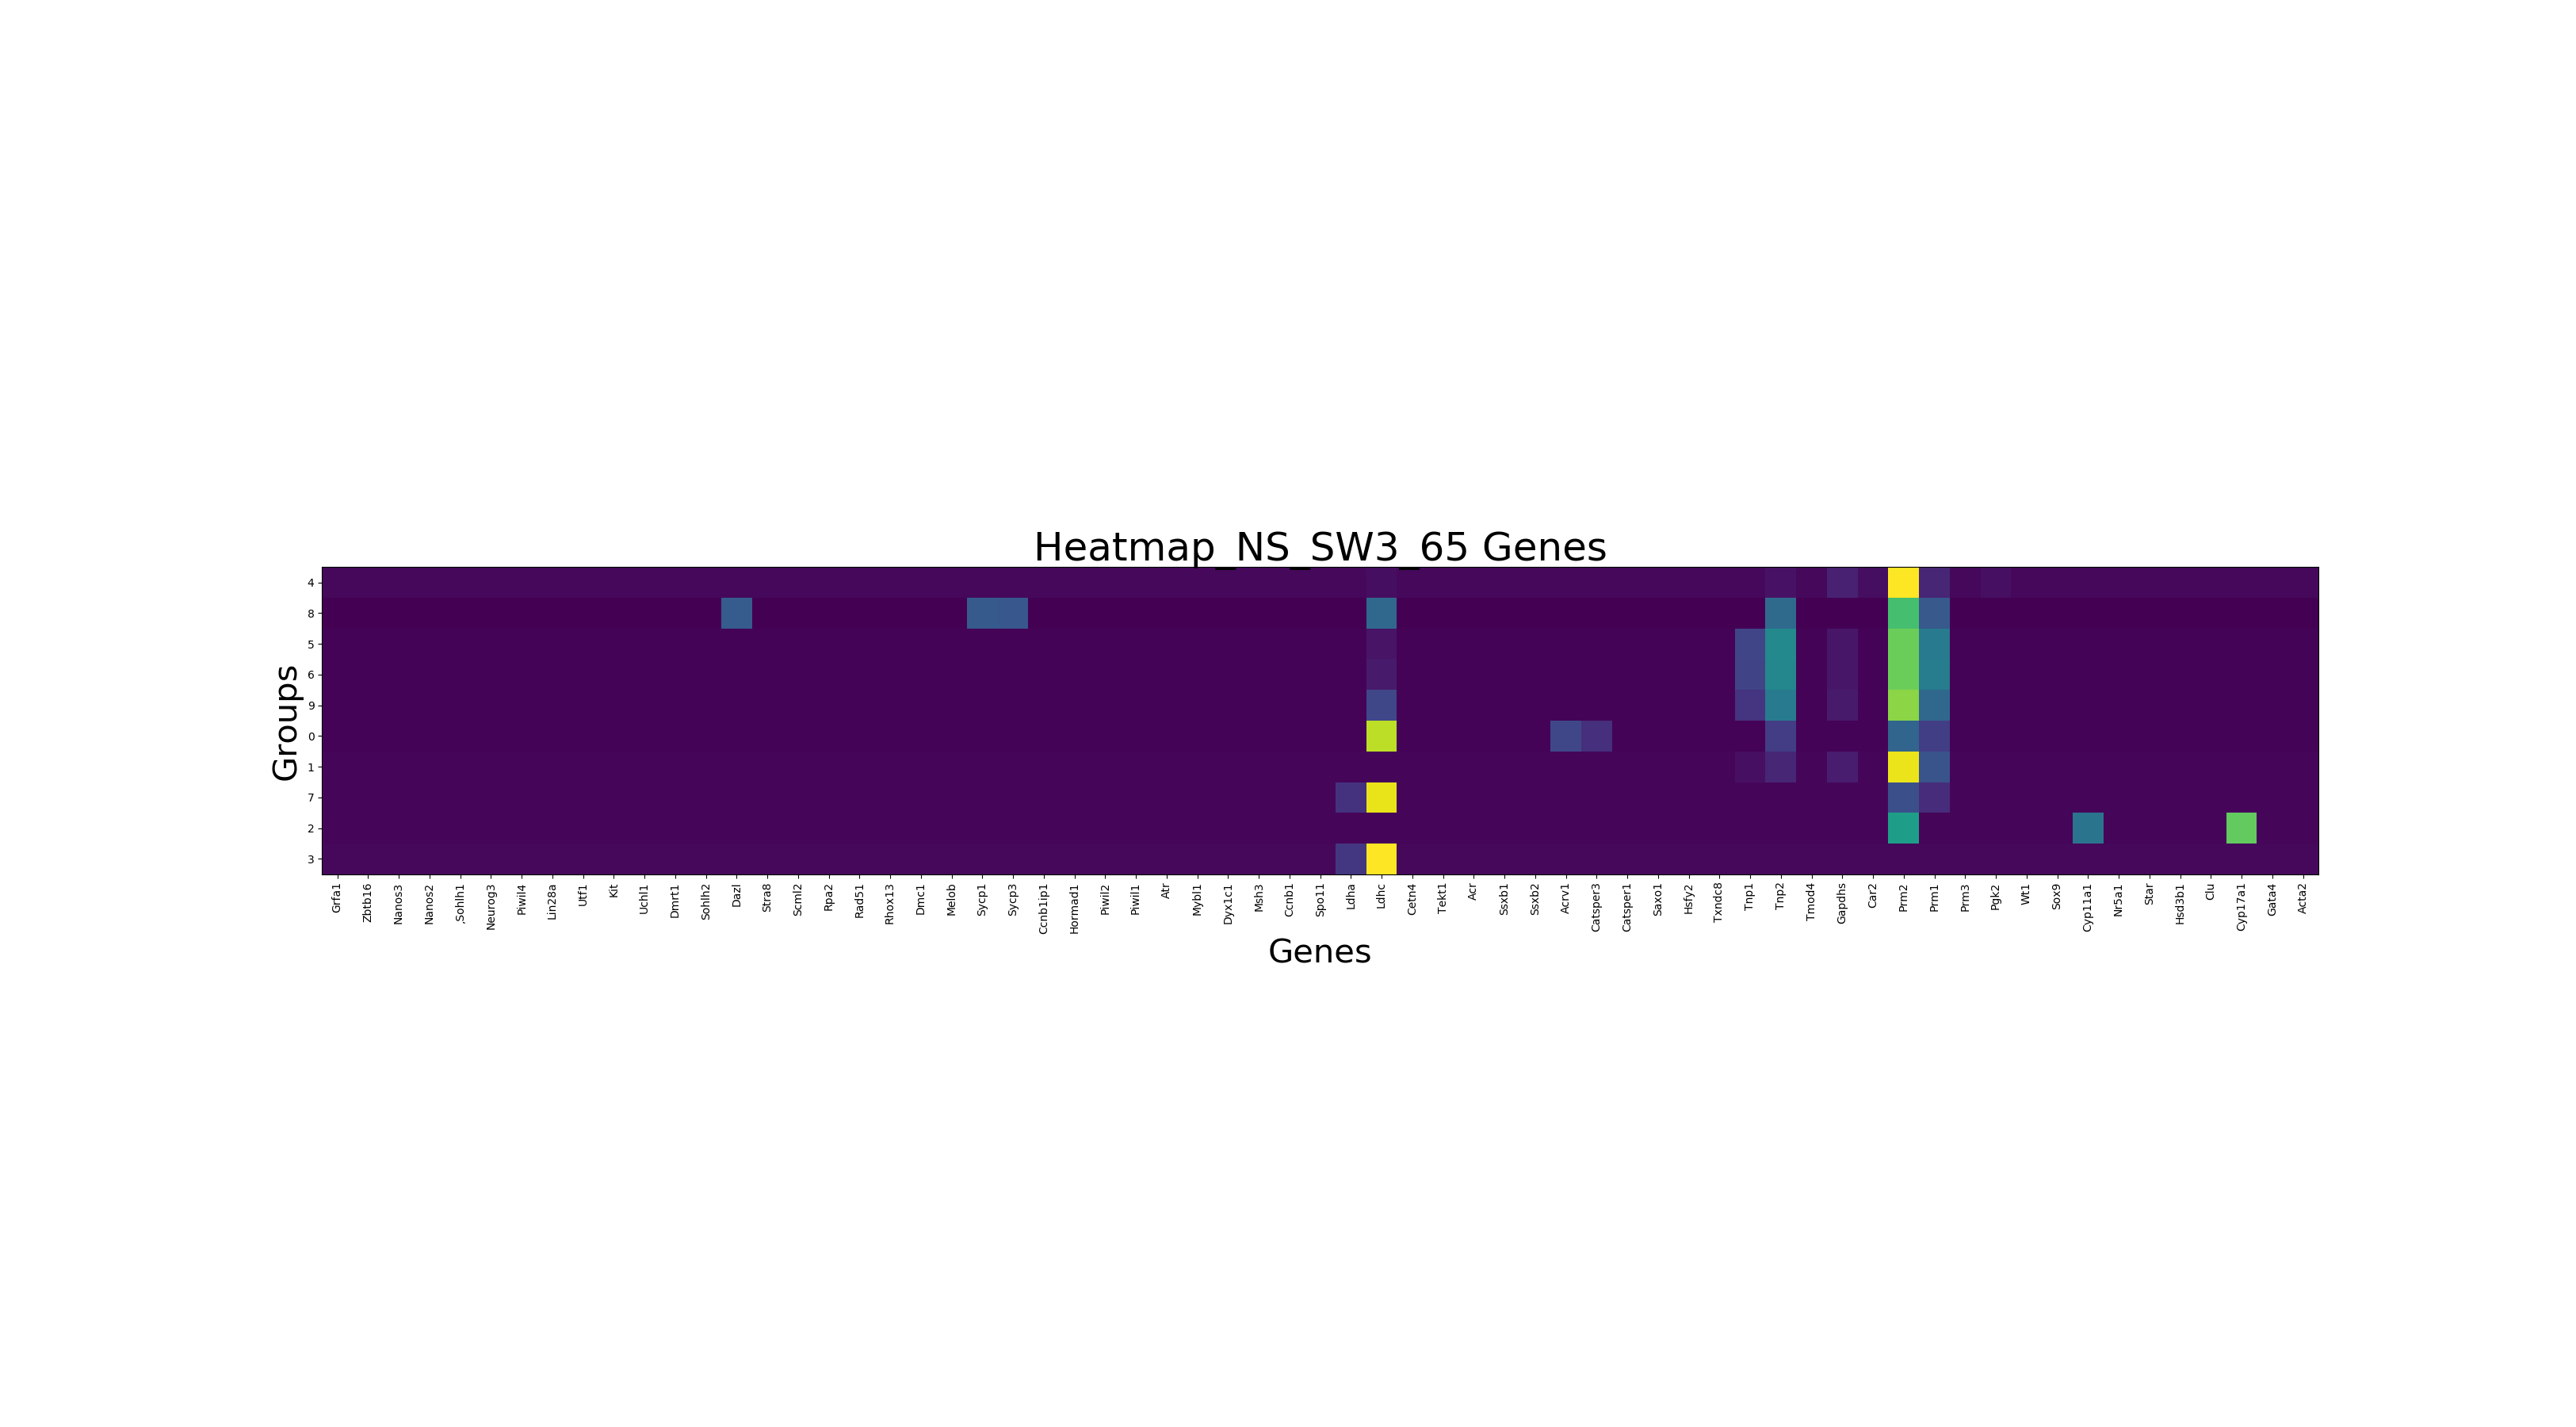
\includegraphics[width=8cm]{figures/Heatmap/65Gene/3.png}
                        &
                        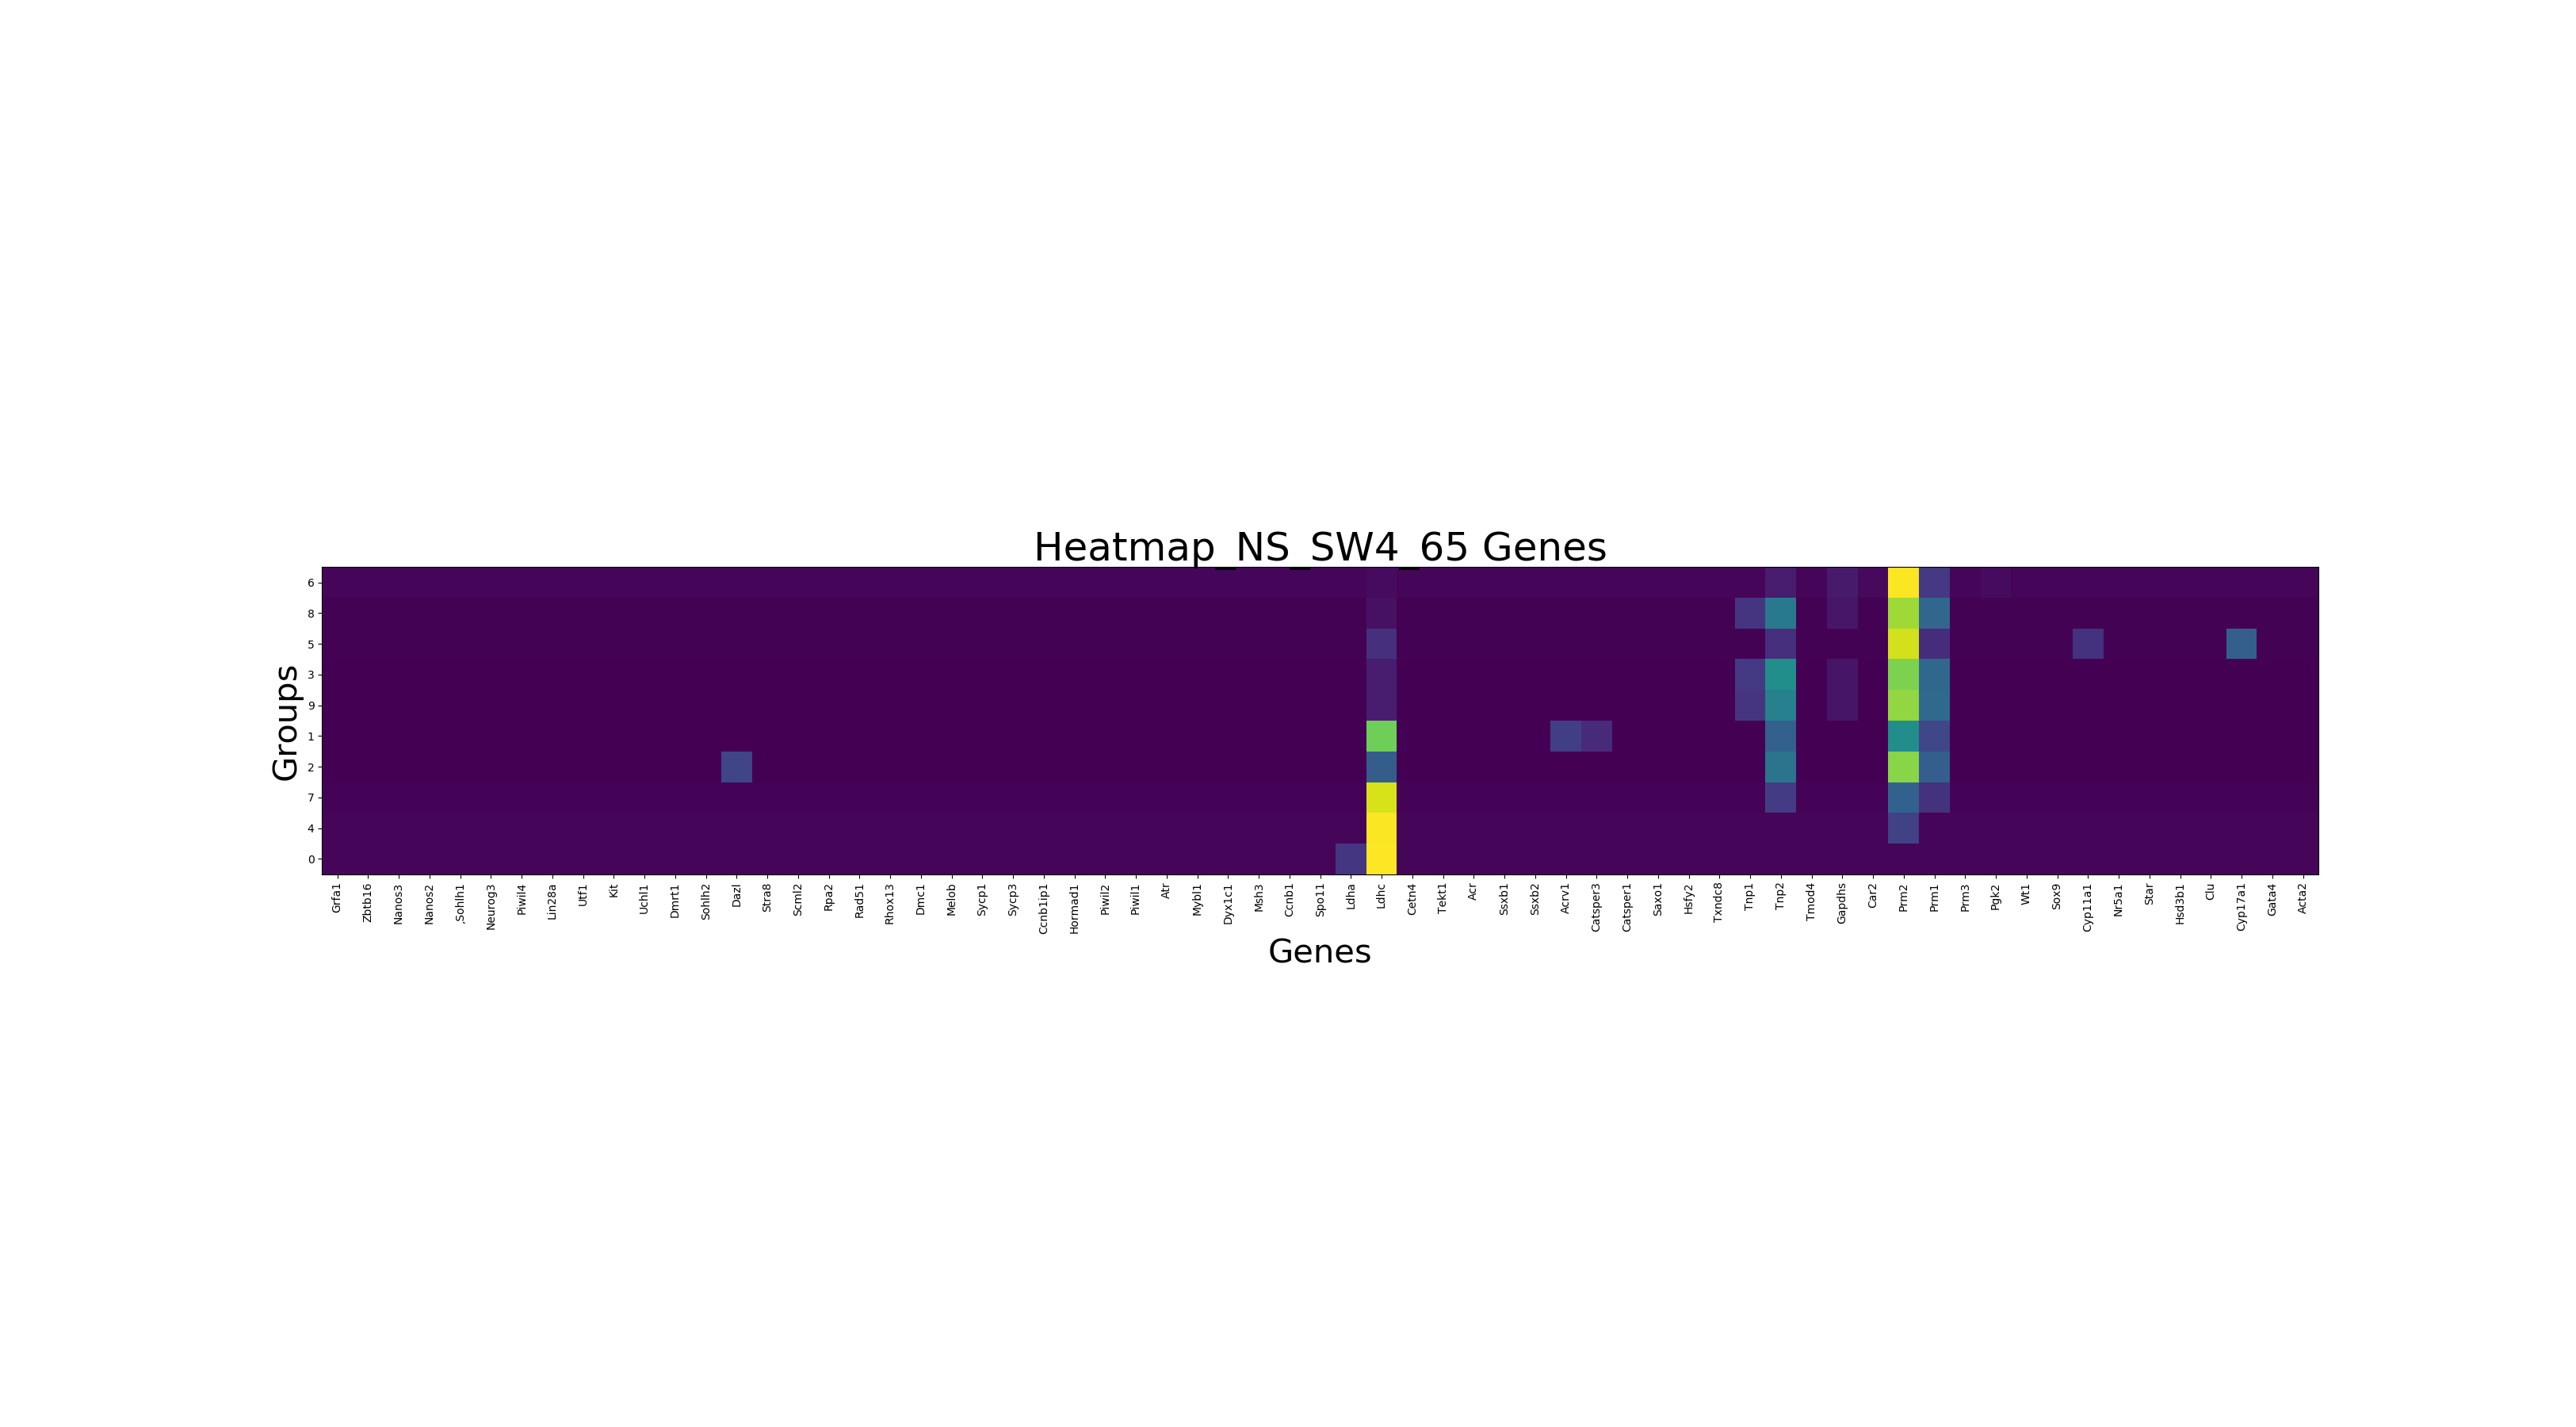
\includegraphics[width=8cm]{figures/Heatmap/65Gene/4.png}
                        \\
                        
                        \mbox{(c) NS\_SW3} & \mbox{(d) NS\_SW4} \\
                    \end{array}$
                    \end{center}
                    \caption{Heatmap Plot of 65 Marker Genes}
                    \label{fig:heat65gene}
                    \end{figure}
            \subsubsection{Top 10 Gene}
                The heatmap plots with the 10 genes which have highest gene expression are in figure \ref{fig:heat10genes}.
                \begin{figure}[hbp]
                    \begin{center}
                        $\begin{array}{cc}
                            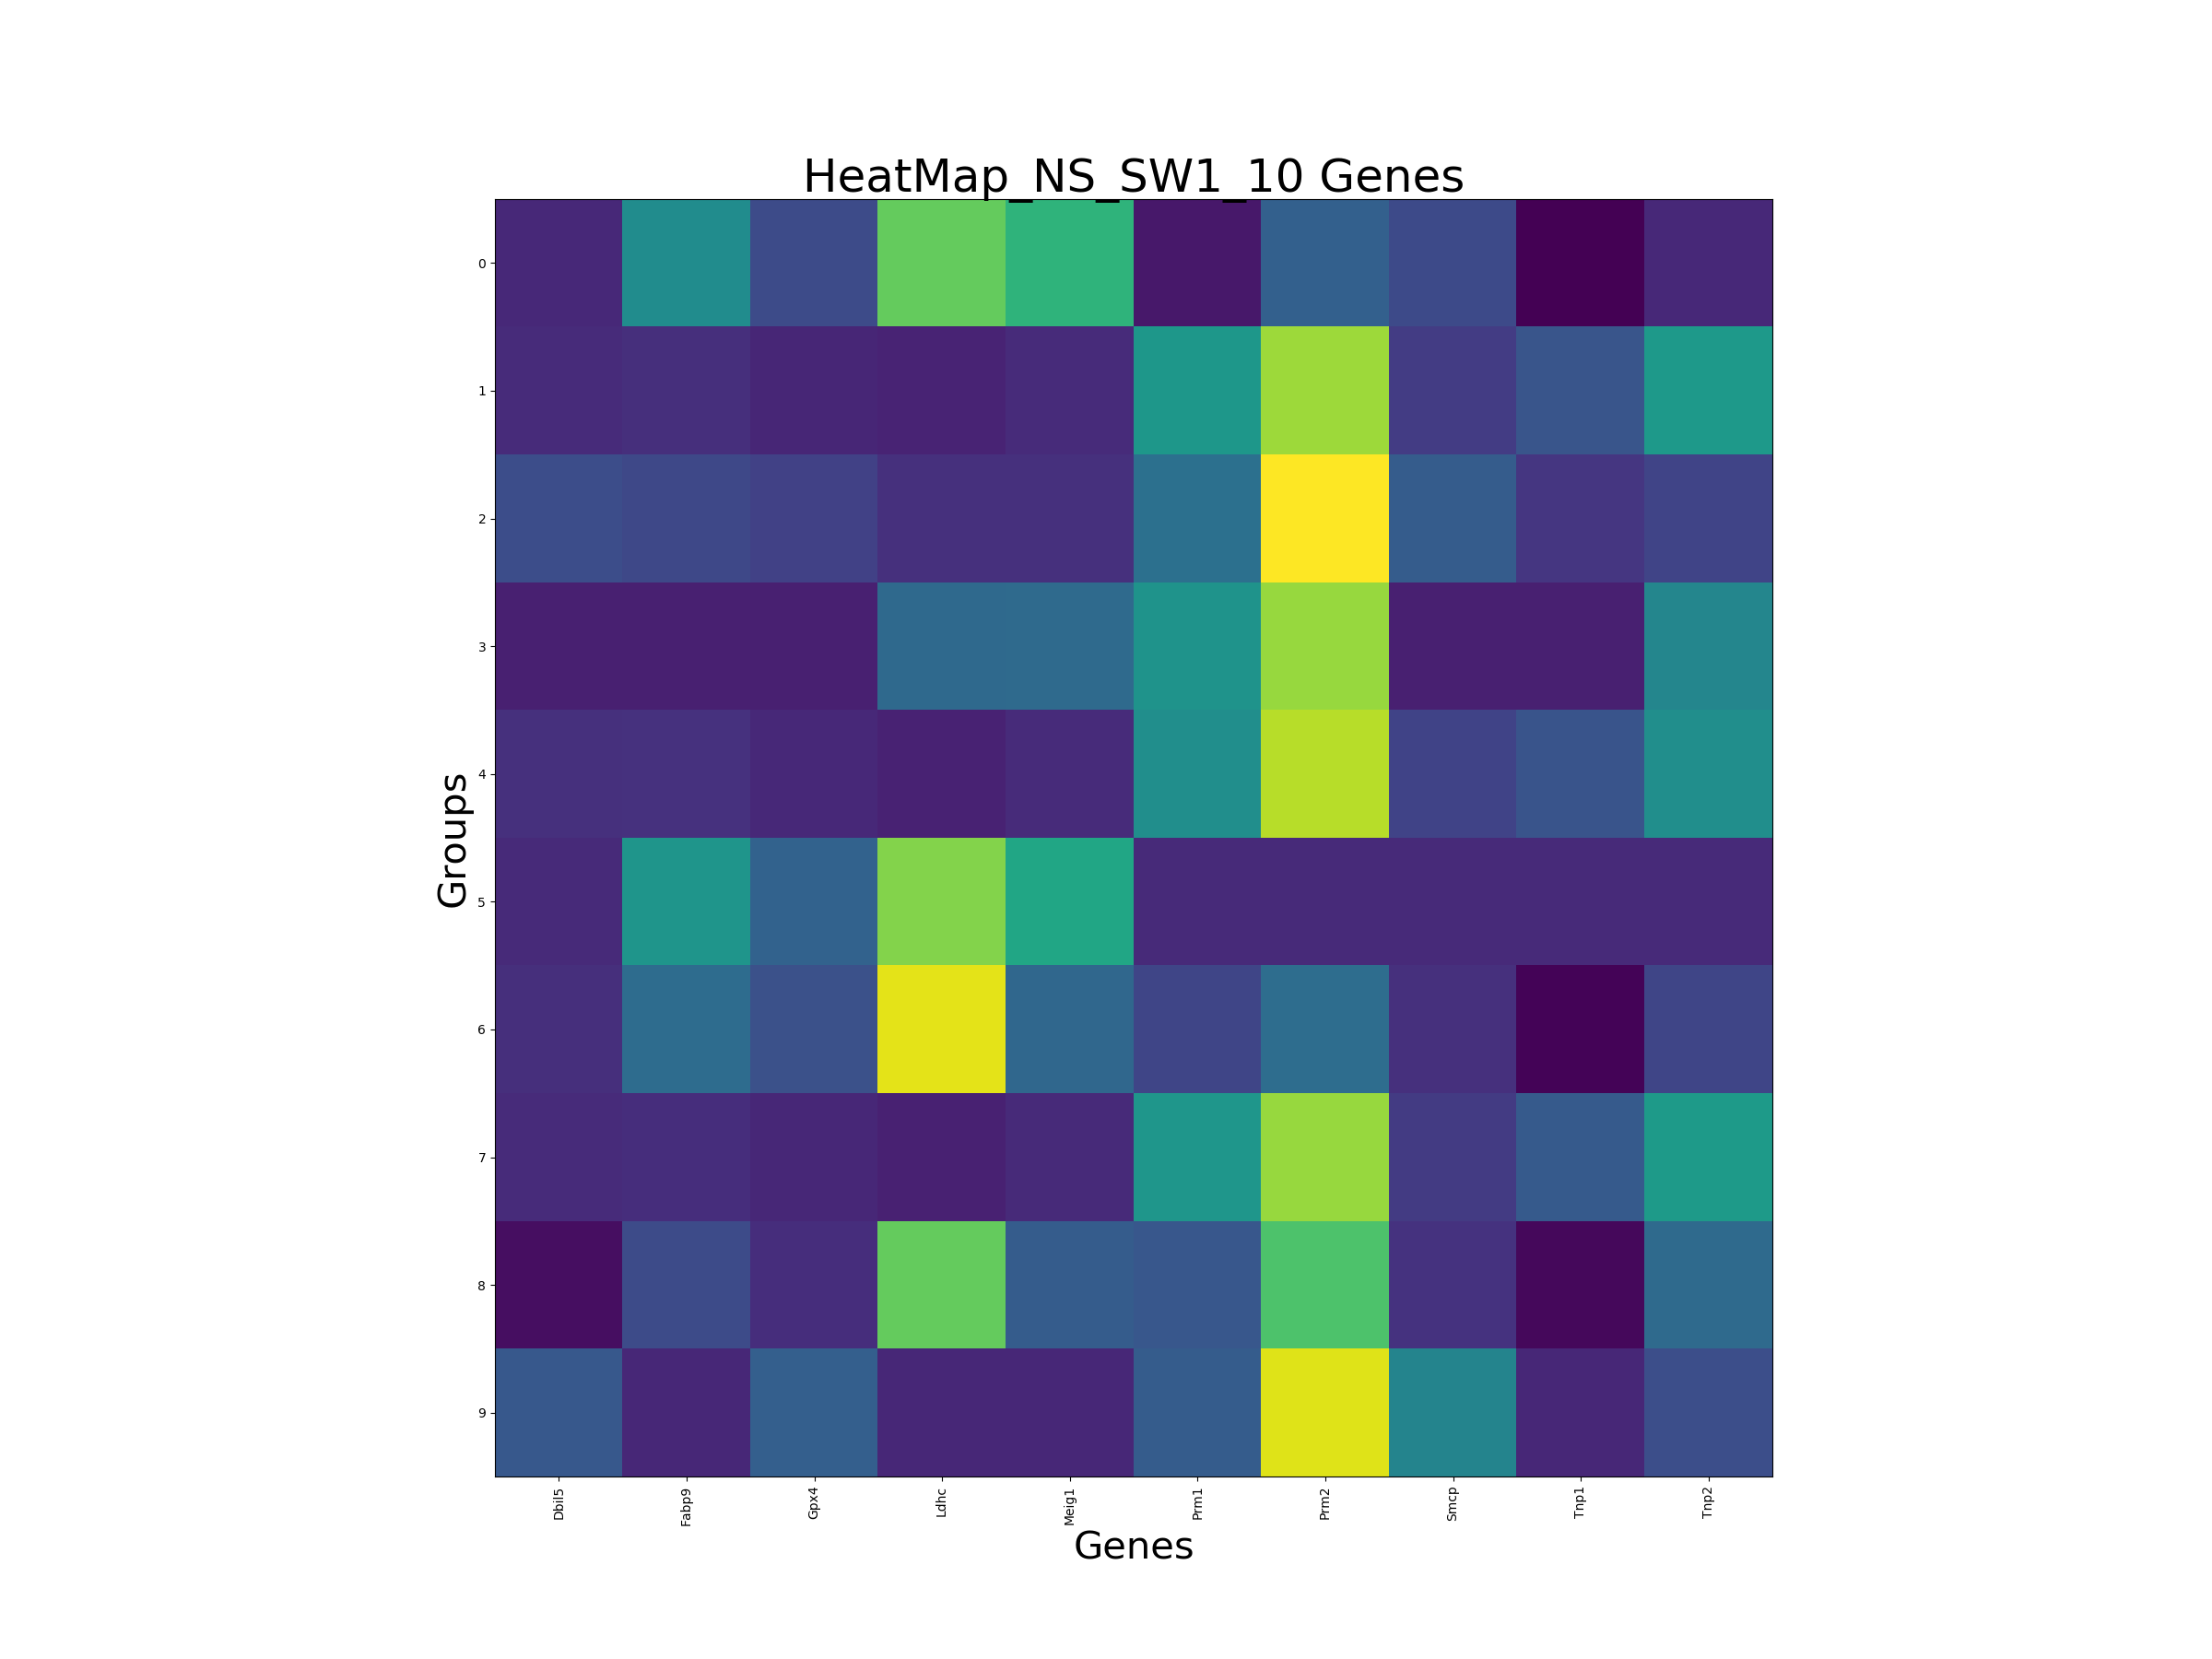
\includegraphics[height=5cm]{figures/Heatmap/Top10/1.png}
                            &
                            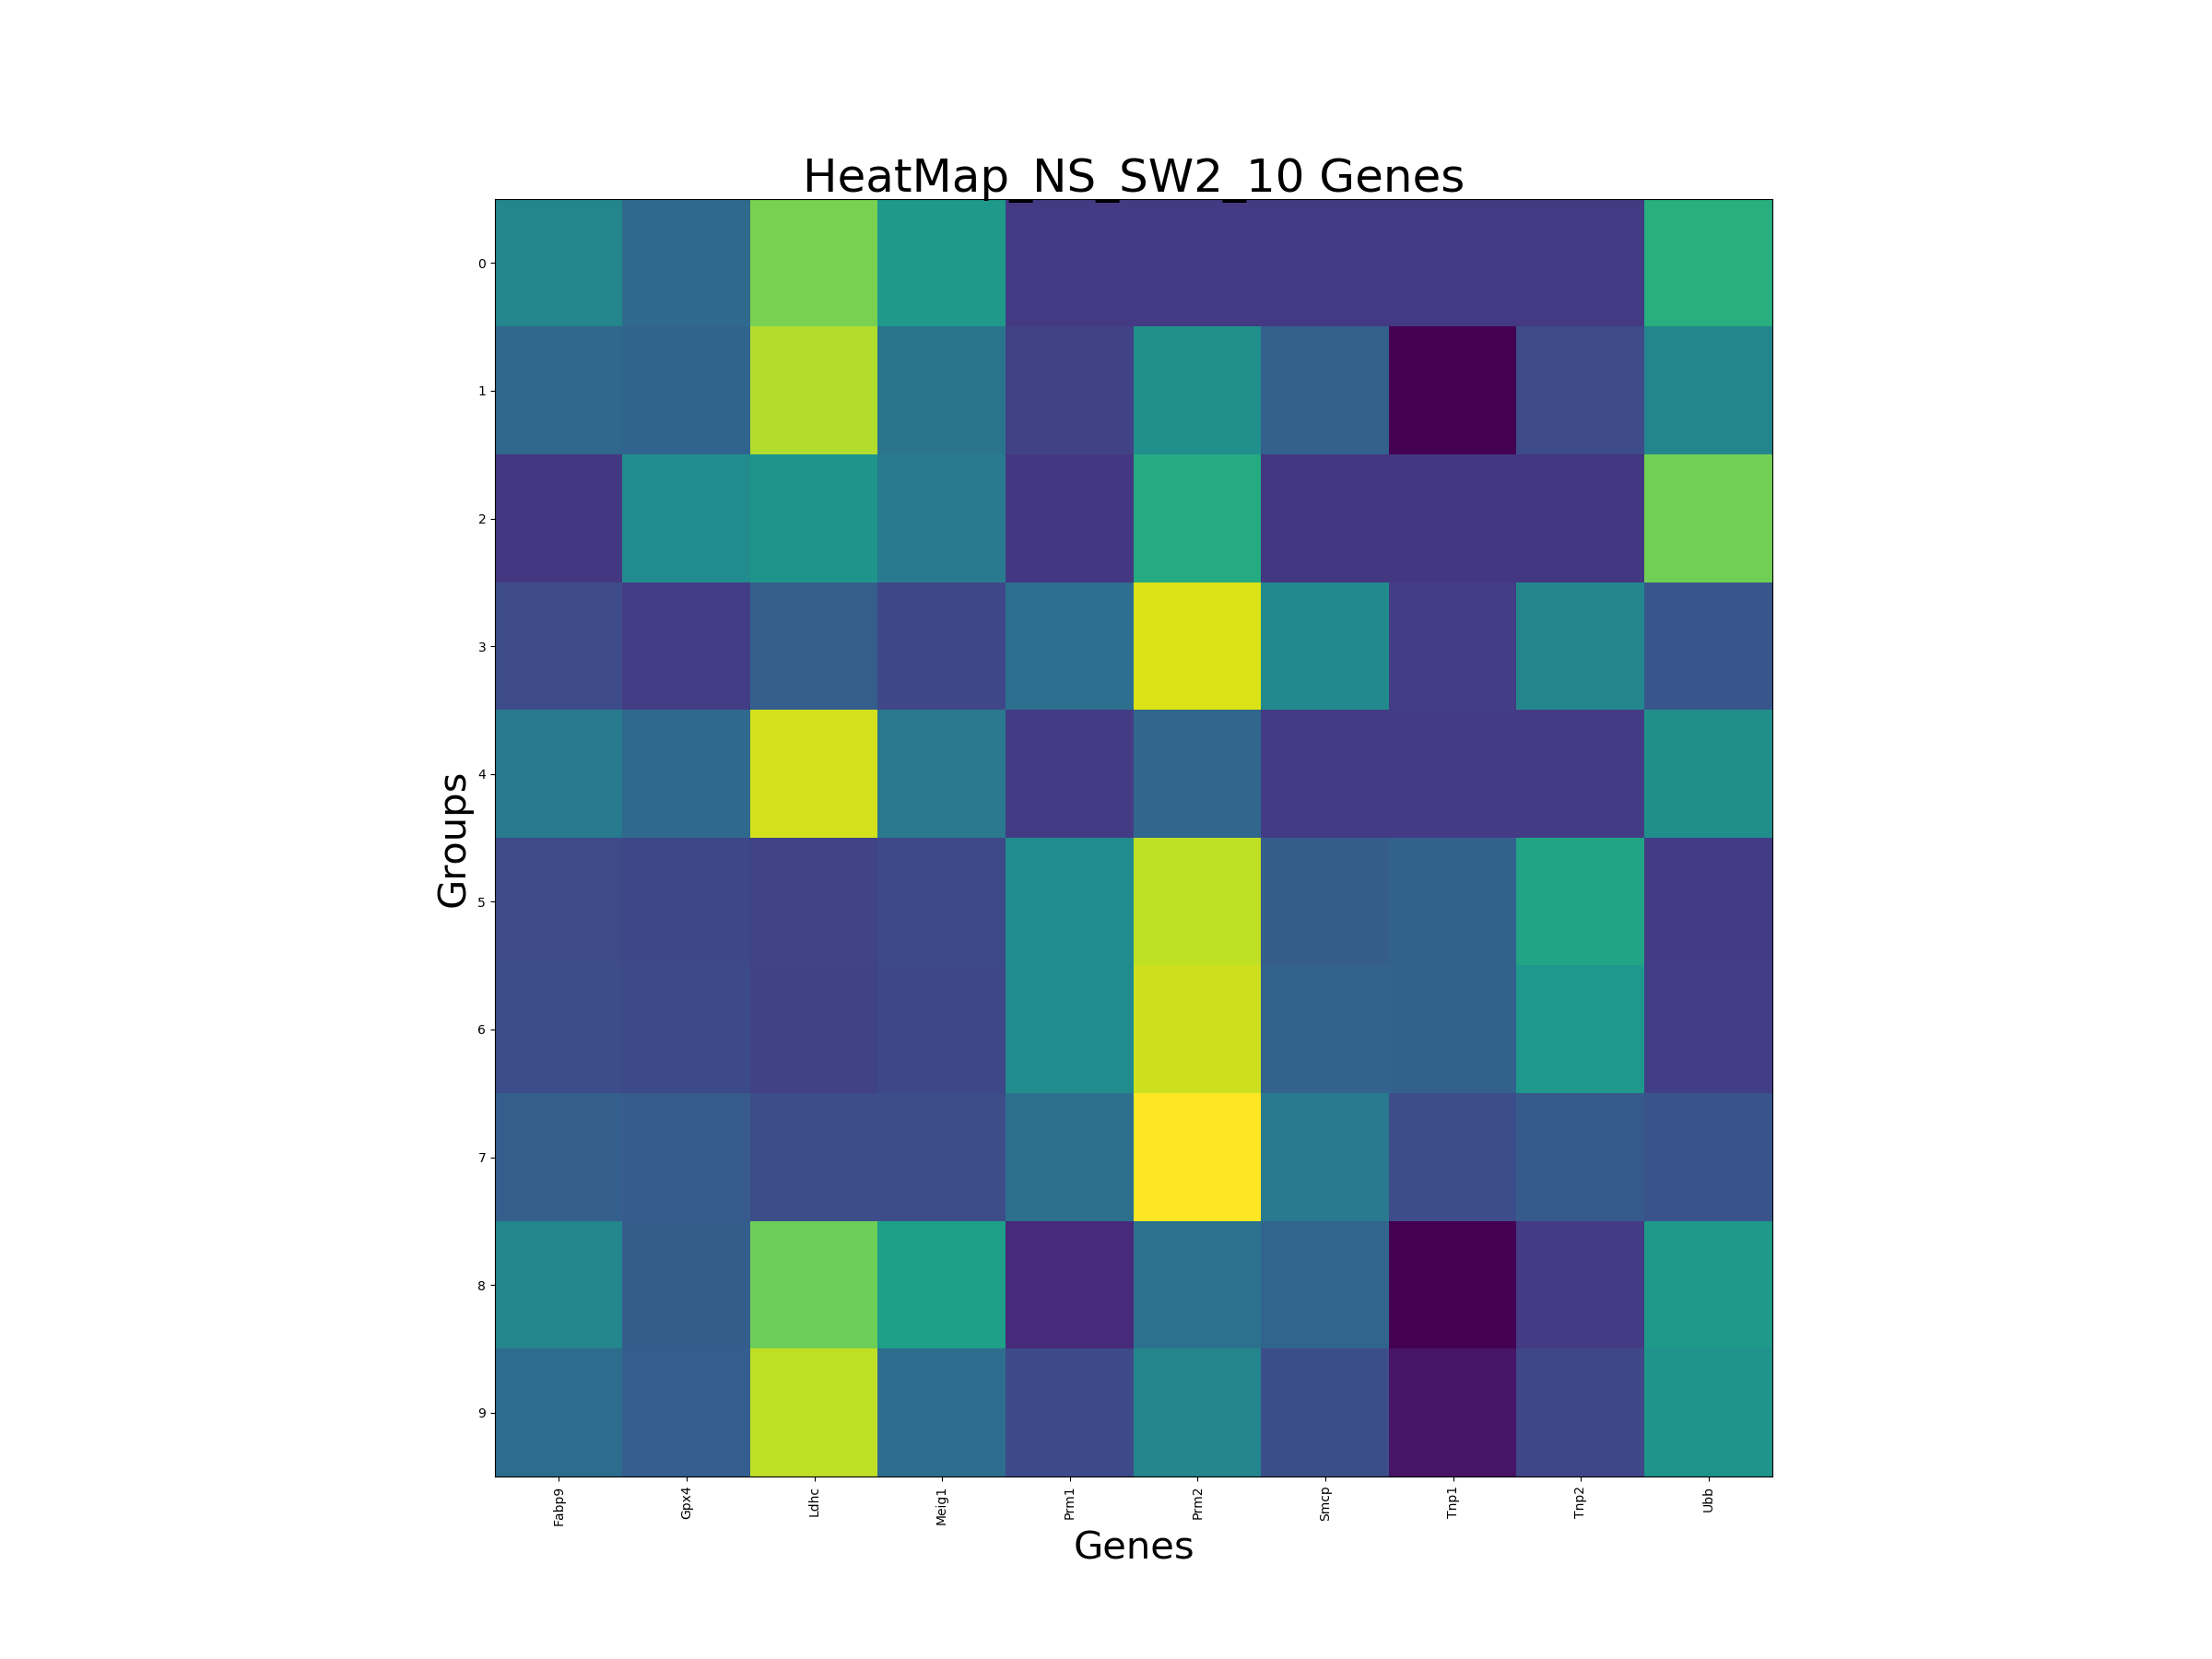
\includegraphics[height=5cm]{figures/Heatmap/Top10/2.png}
                            \\
                            
                            \mbox{(a) NS\_SW1} & \mbox{(b) NS\_SW2} \\
                            
                            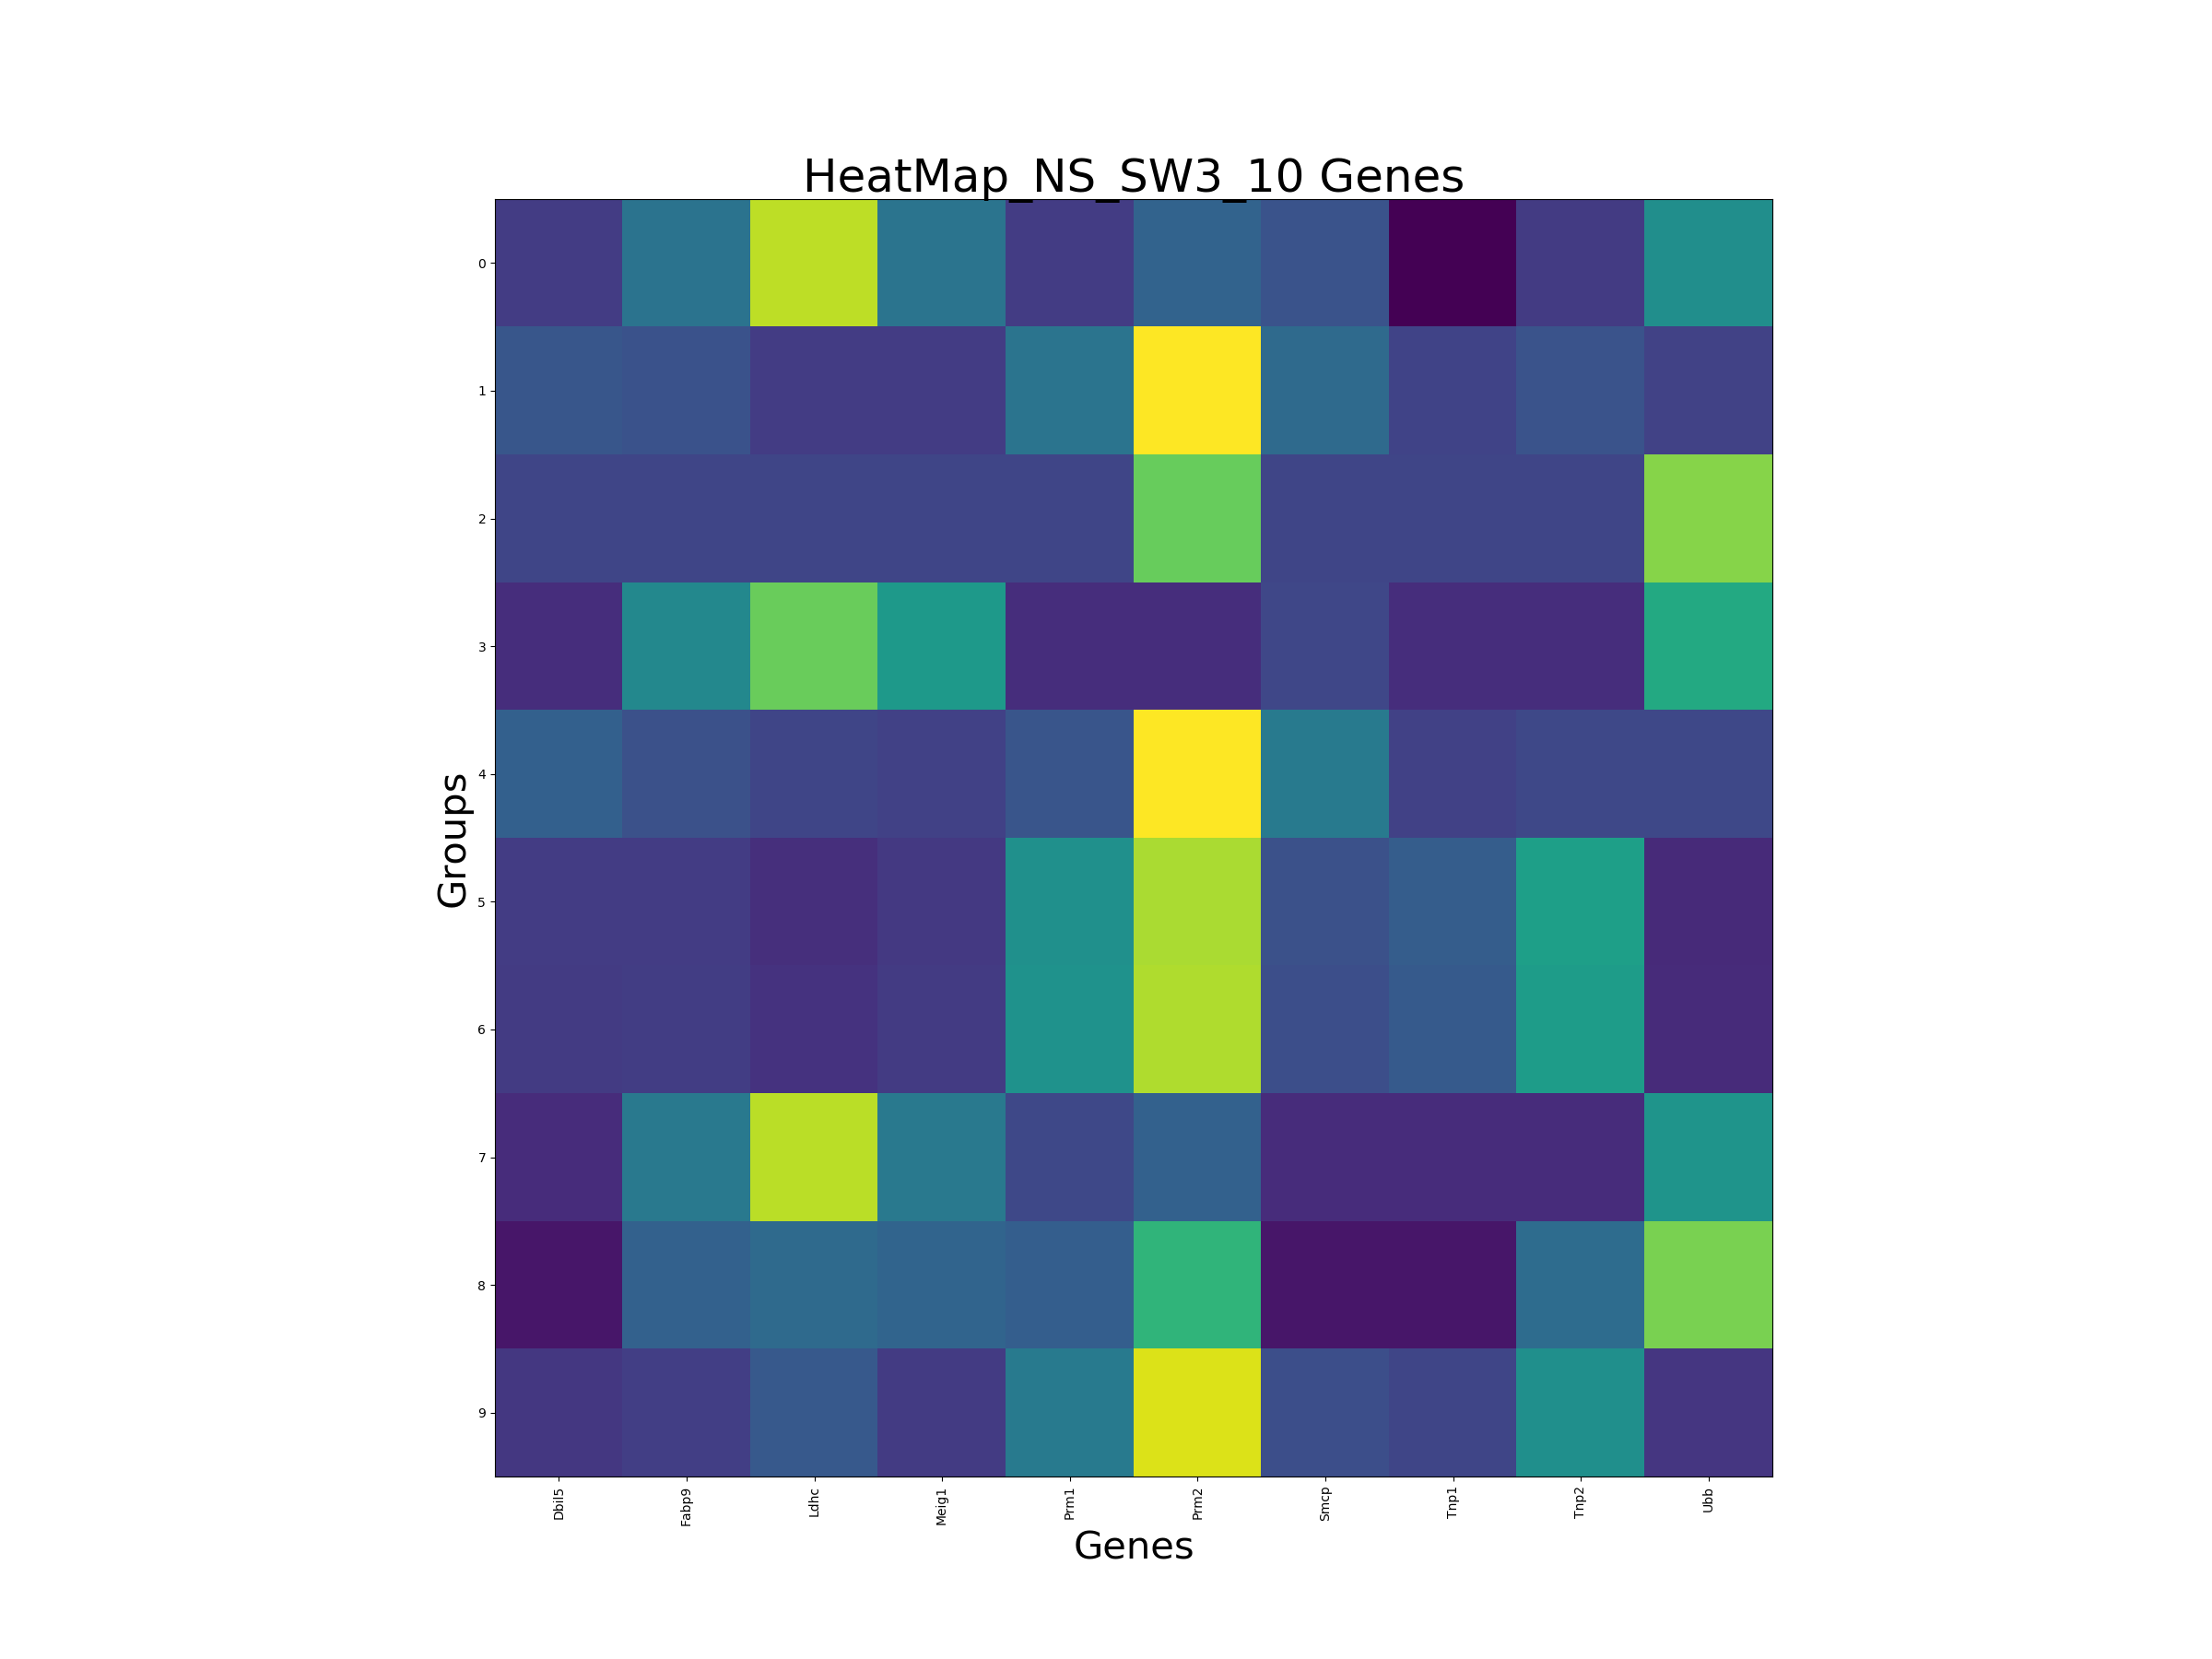
\includegraphics[height=5cm]{figures/Heatmap/Top10/3.png}
                            &
                            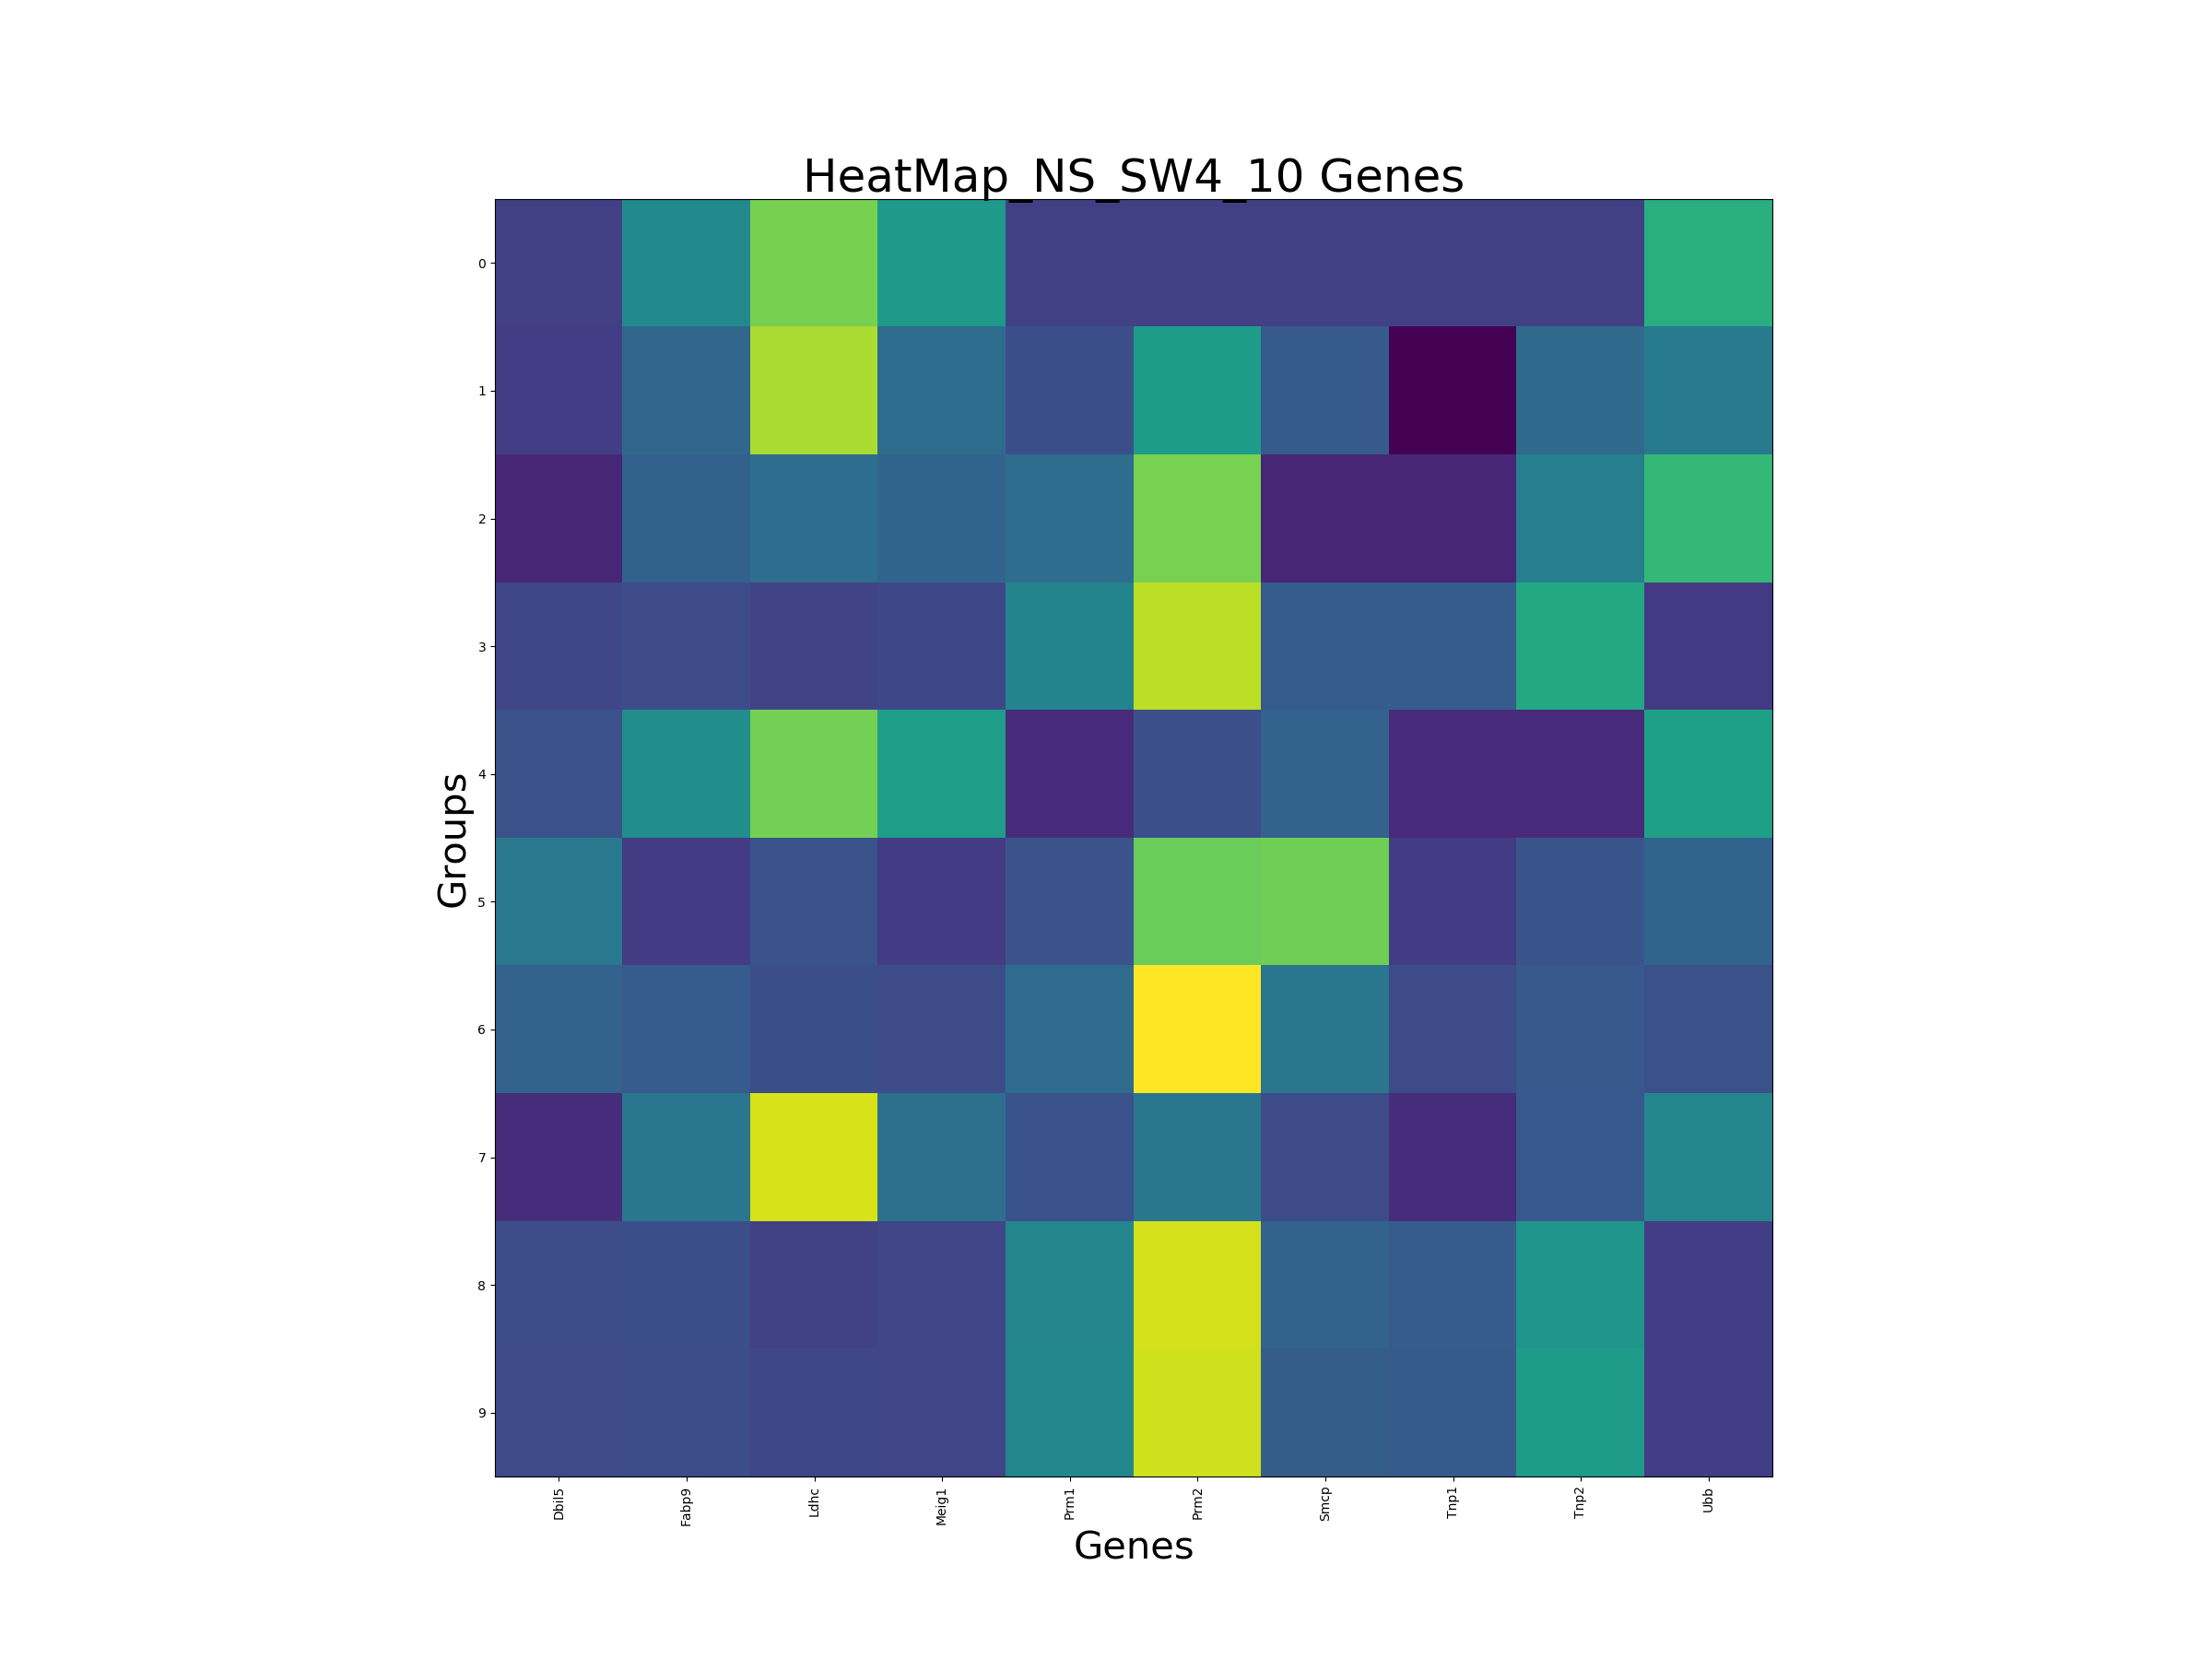
\includegraphics[height=5cm]{figures/Heatmap/Top10/4.png}
                            \\
                            
                            \mbox{(c) NS\_SW3} & \mbox{(d) NS\_SW4} \\
                        \end{array}$
                    \end{center}
                    \caption{Heatmap Plot of 10 Genes which have Highest Expression}
                    \label{fig:heat10genes}
                \end{figure}
        
        \subsection{Pseudo-time}
            According to gene expression level, I can derive an order of each cluster, in other words, pseudo-time. 
            \subsubsection{12 Genes}
                The pseudo-time plots with 12 marker genes are in figure \ref{fig:time12gene}.
                \begin{figure}[hbp]
                    \begin{center}
                        $\begin{array}{cc}
                            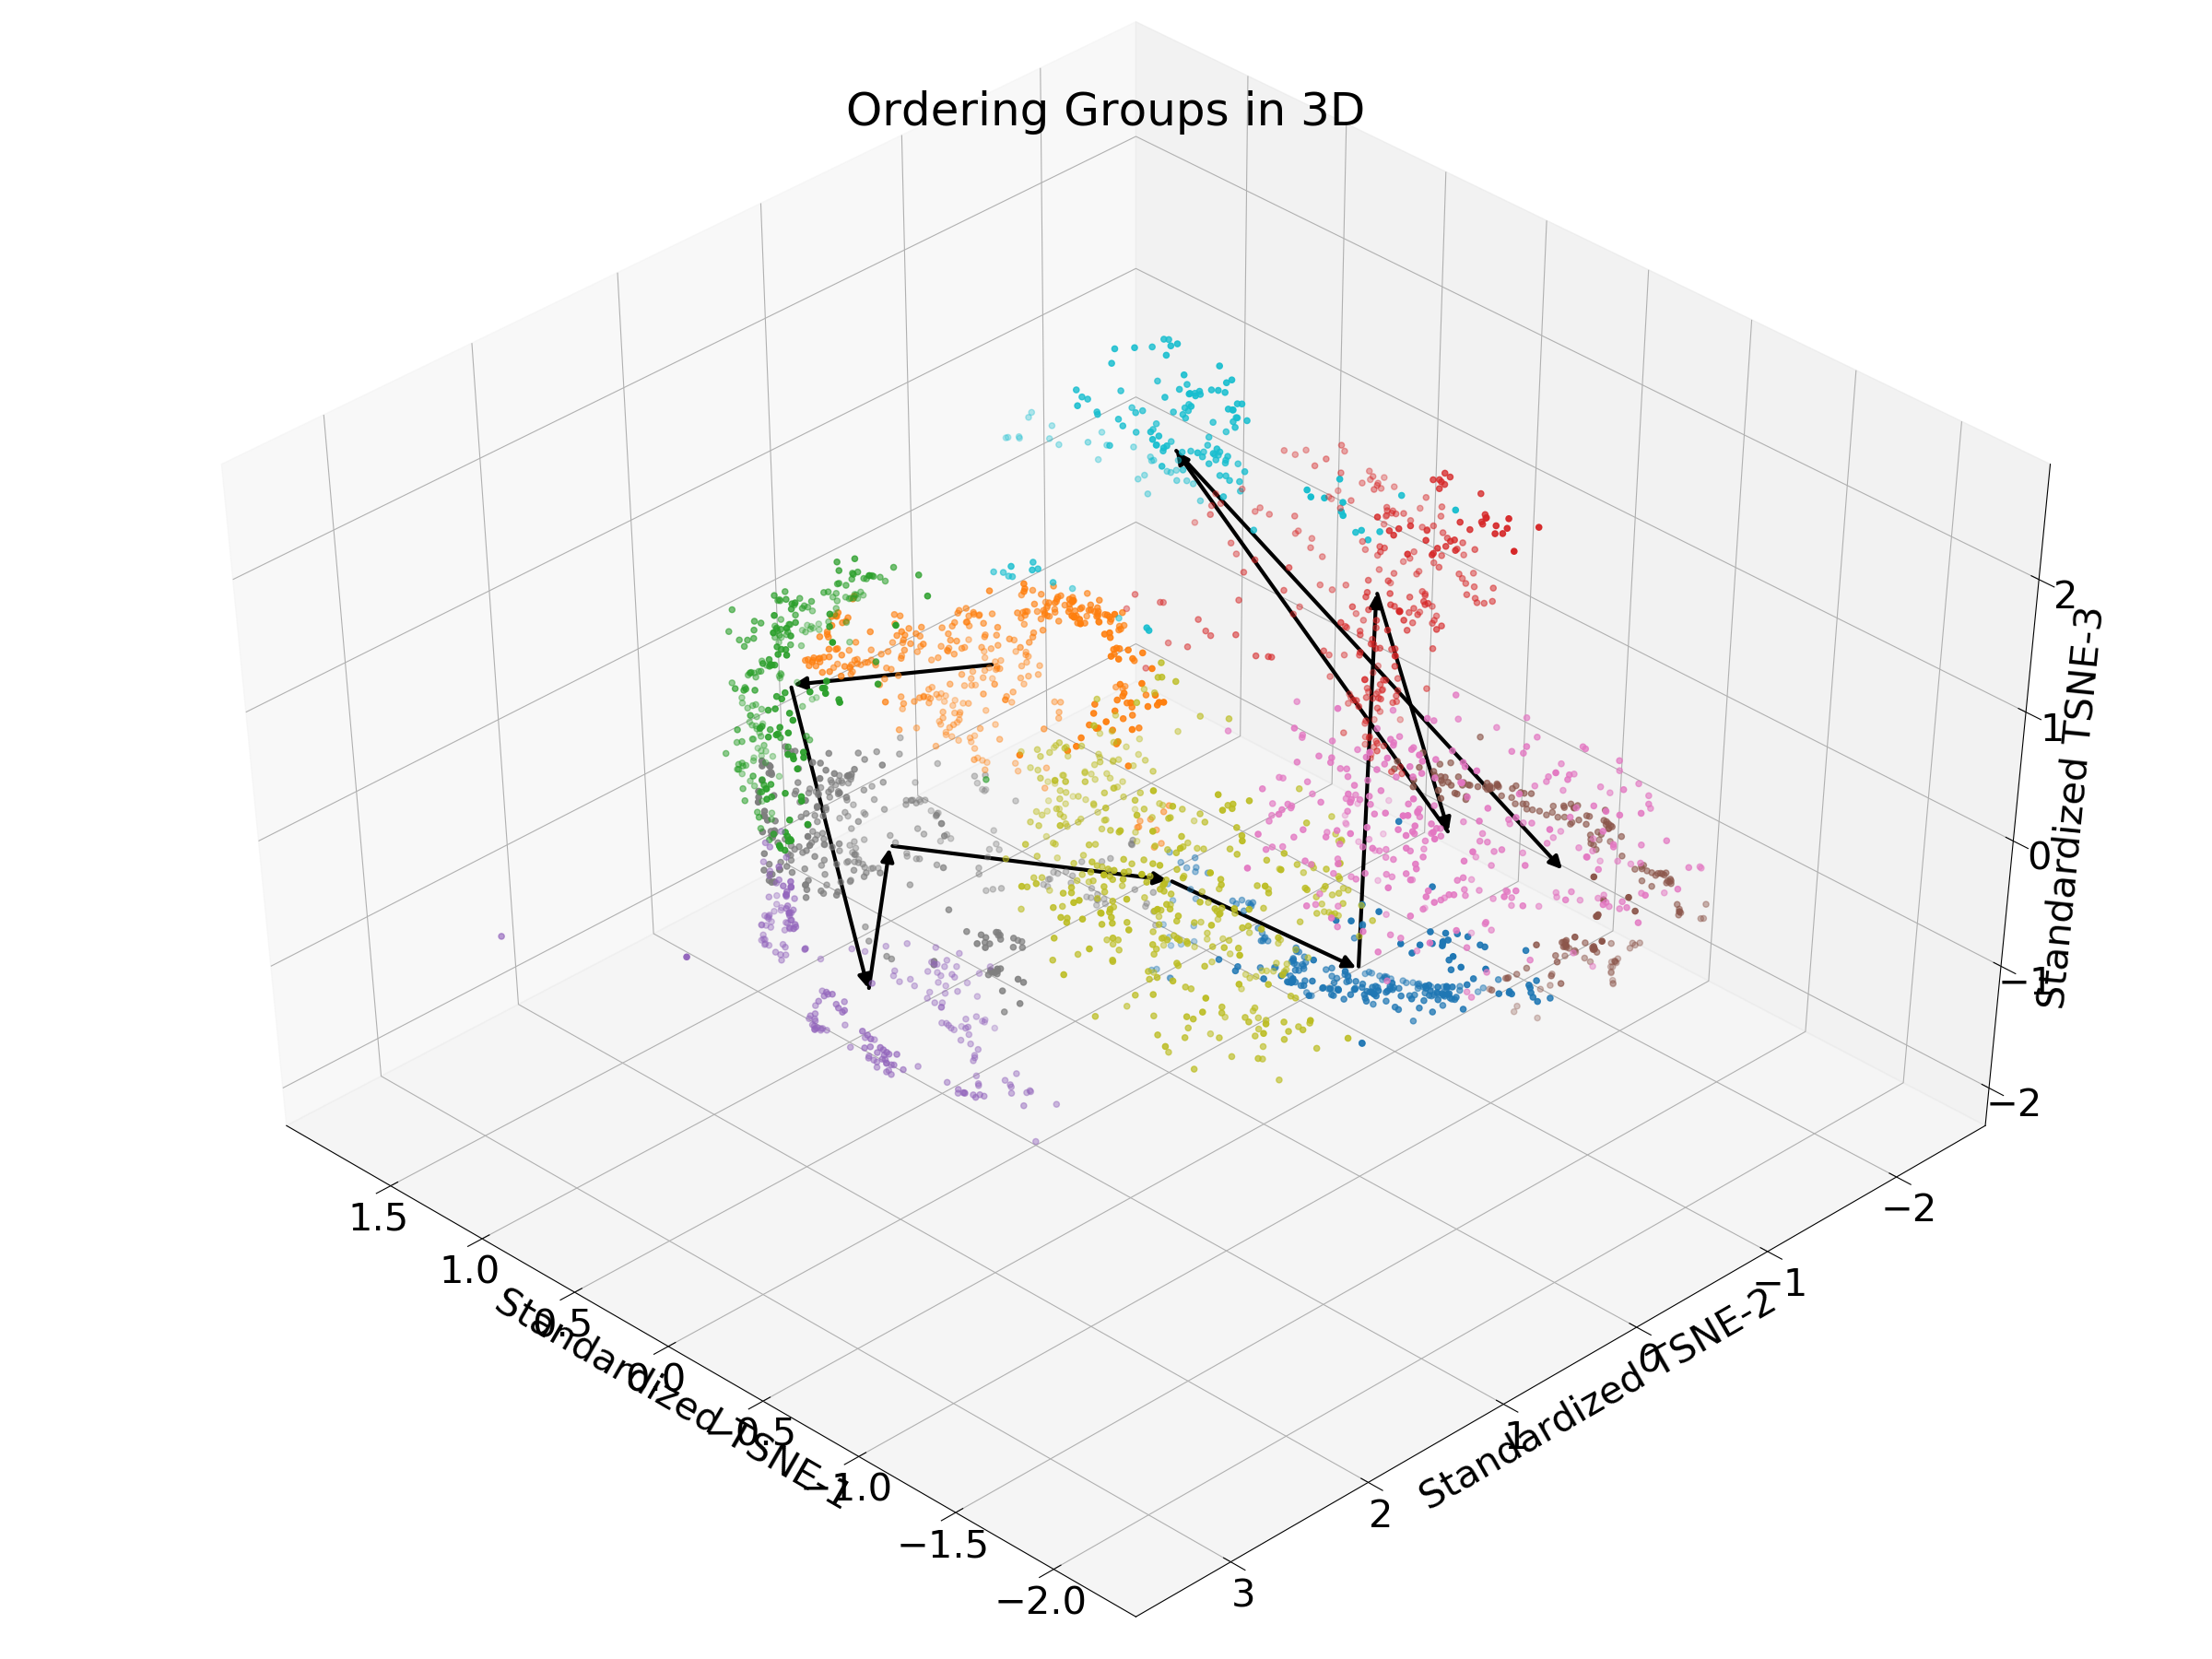
\includegraphics[height=5cm]{figures/Pseudotime/12Gene/1.png}
                            &
                            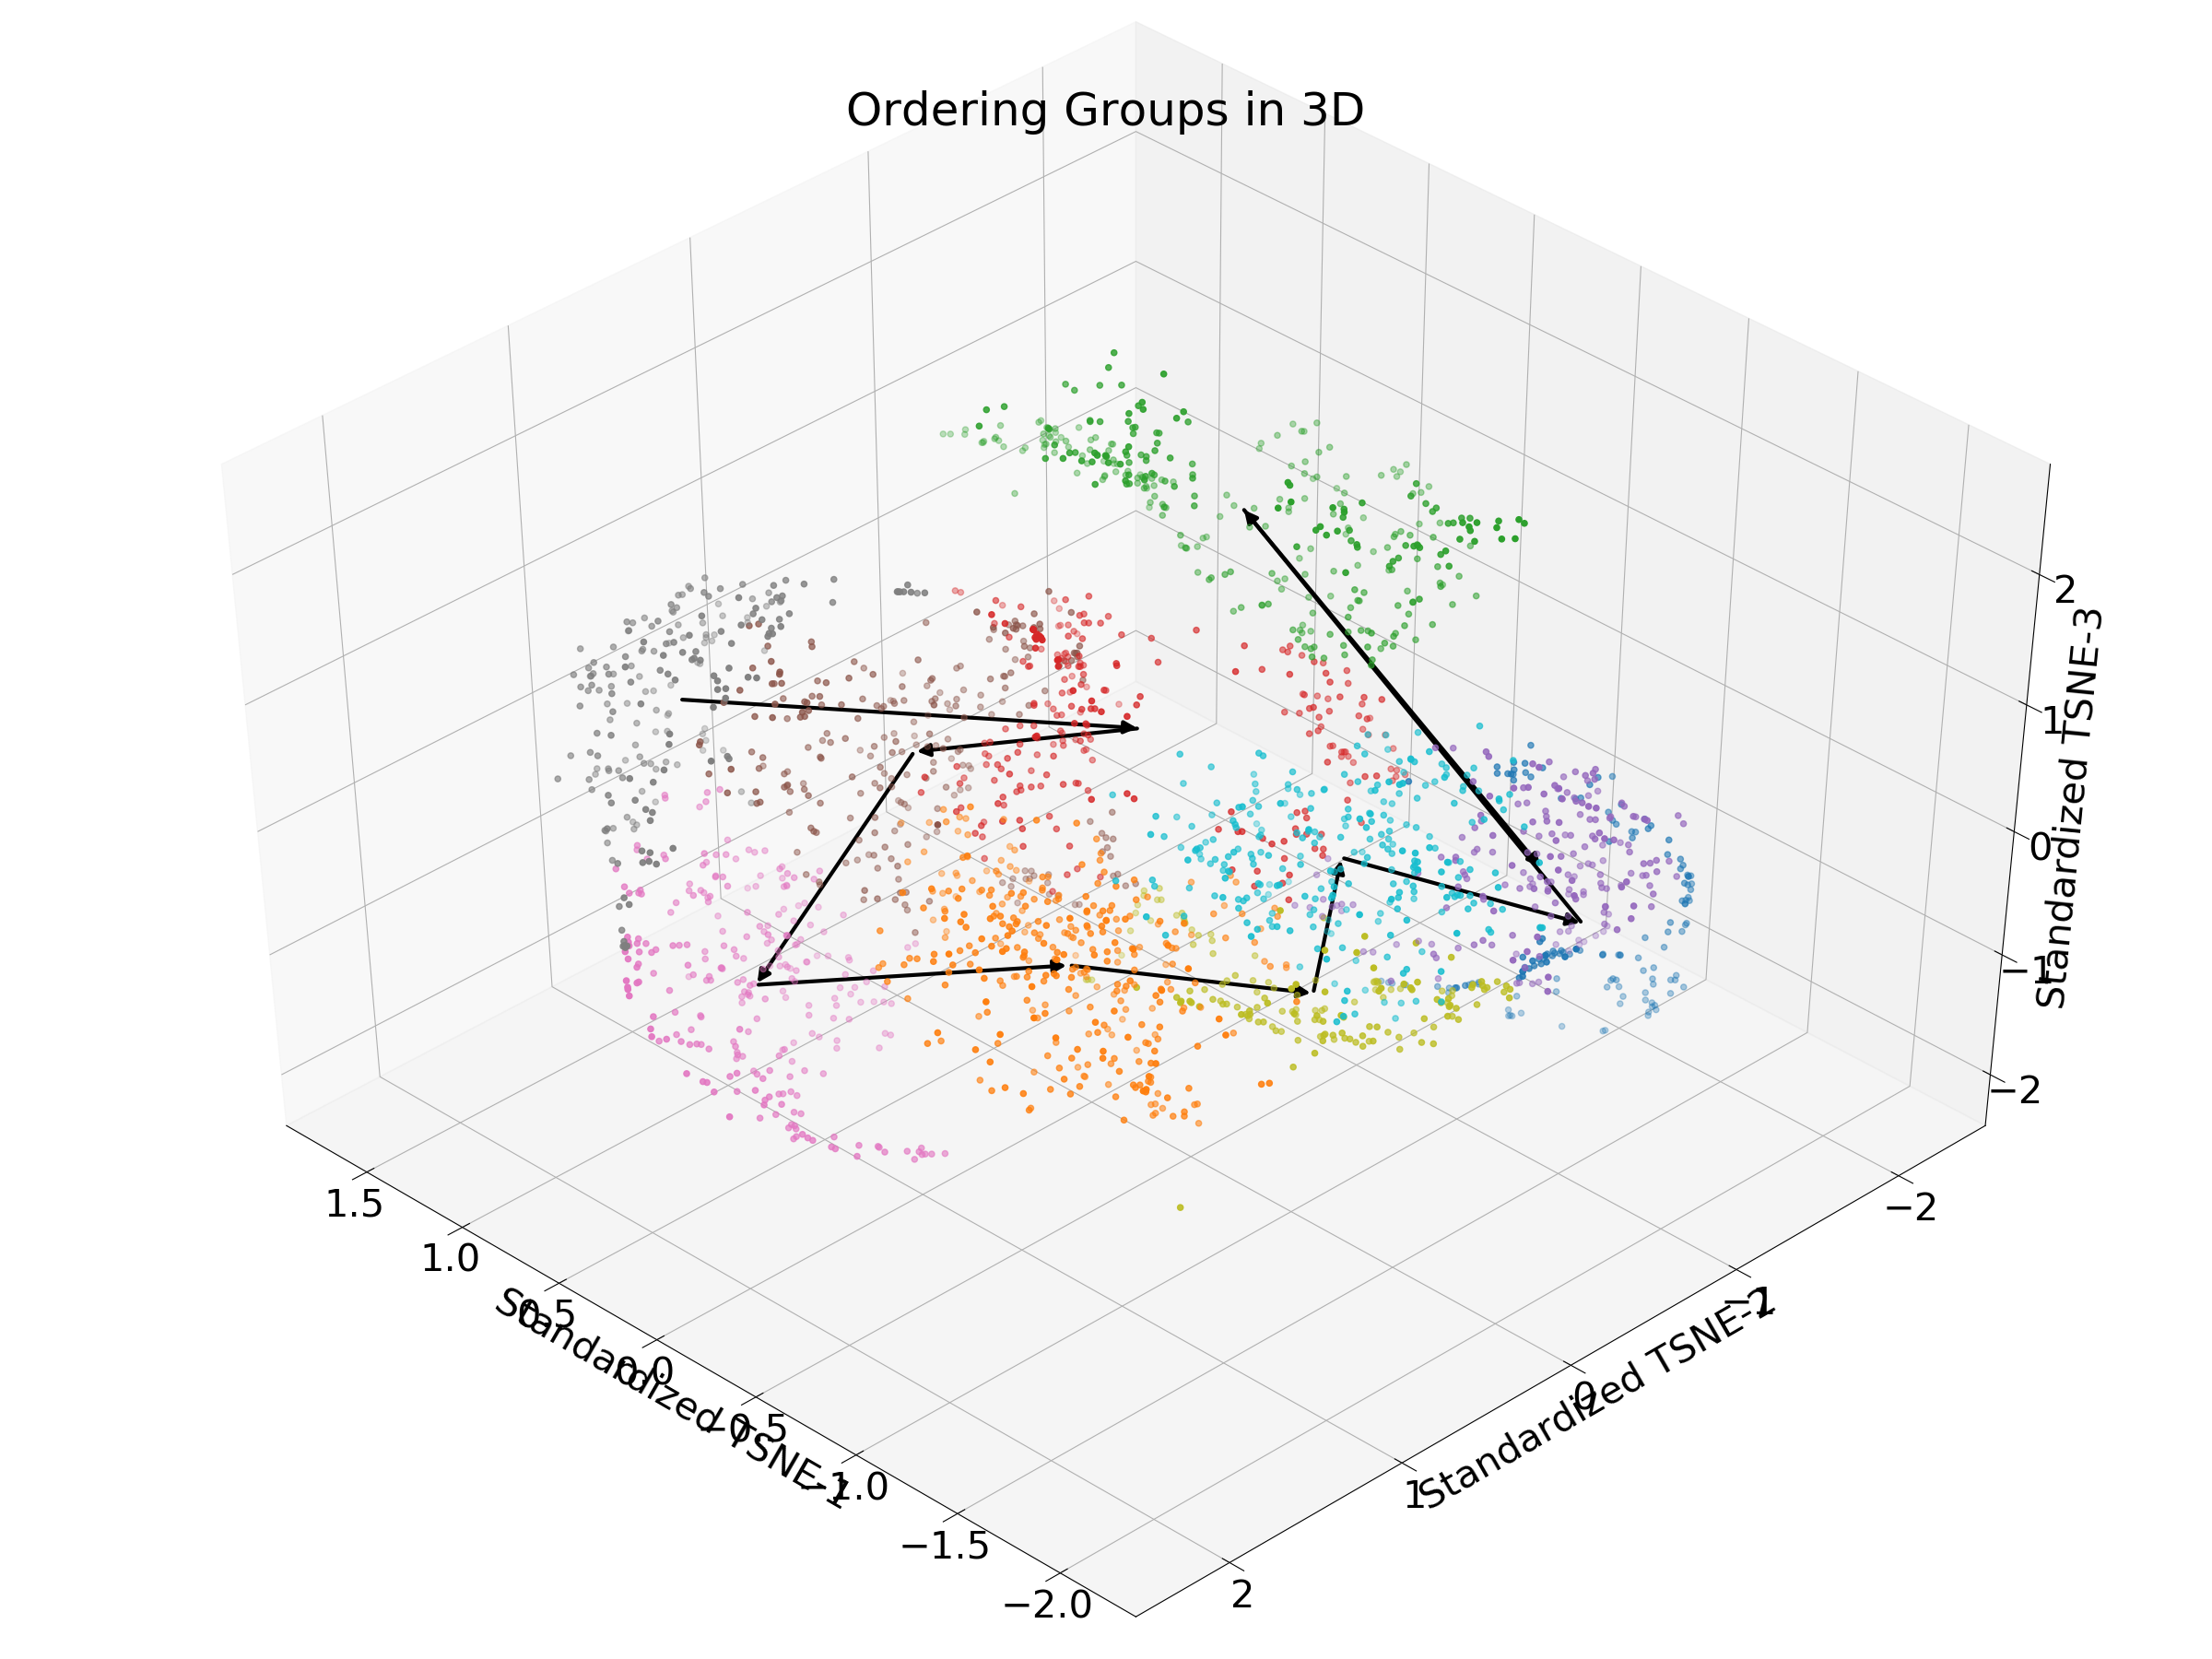
\includegraphics[height=5cm]{figures/Pseudotime/12Gene/2.png}
                            \\
                            
                            \mbox{(a) NS\_SW1} & \mbox{(b) NS\_SW2} \\
                            
                            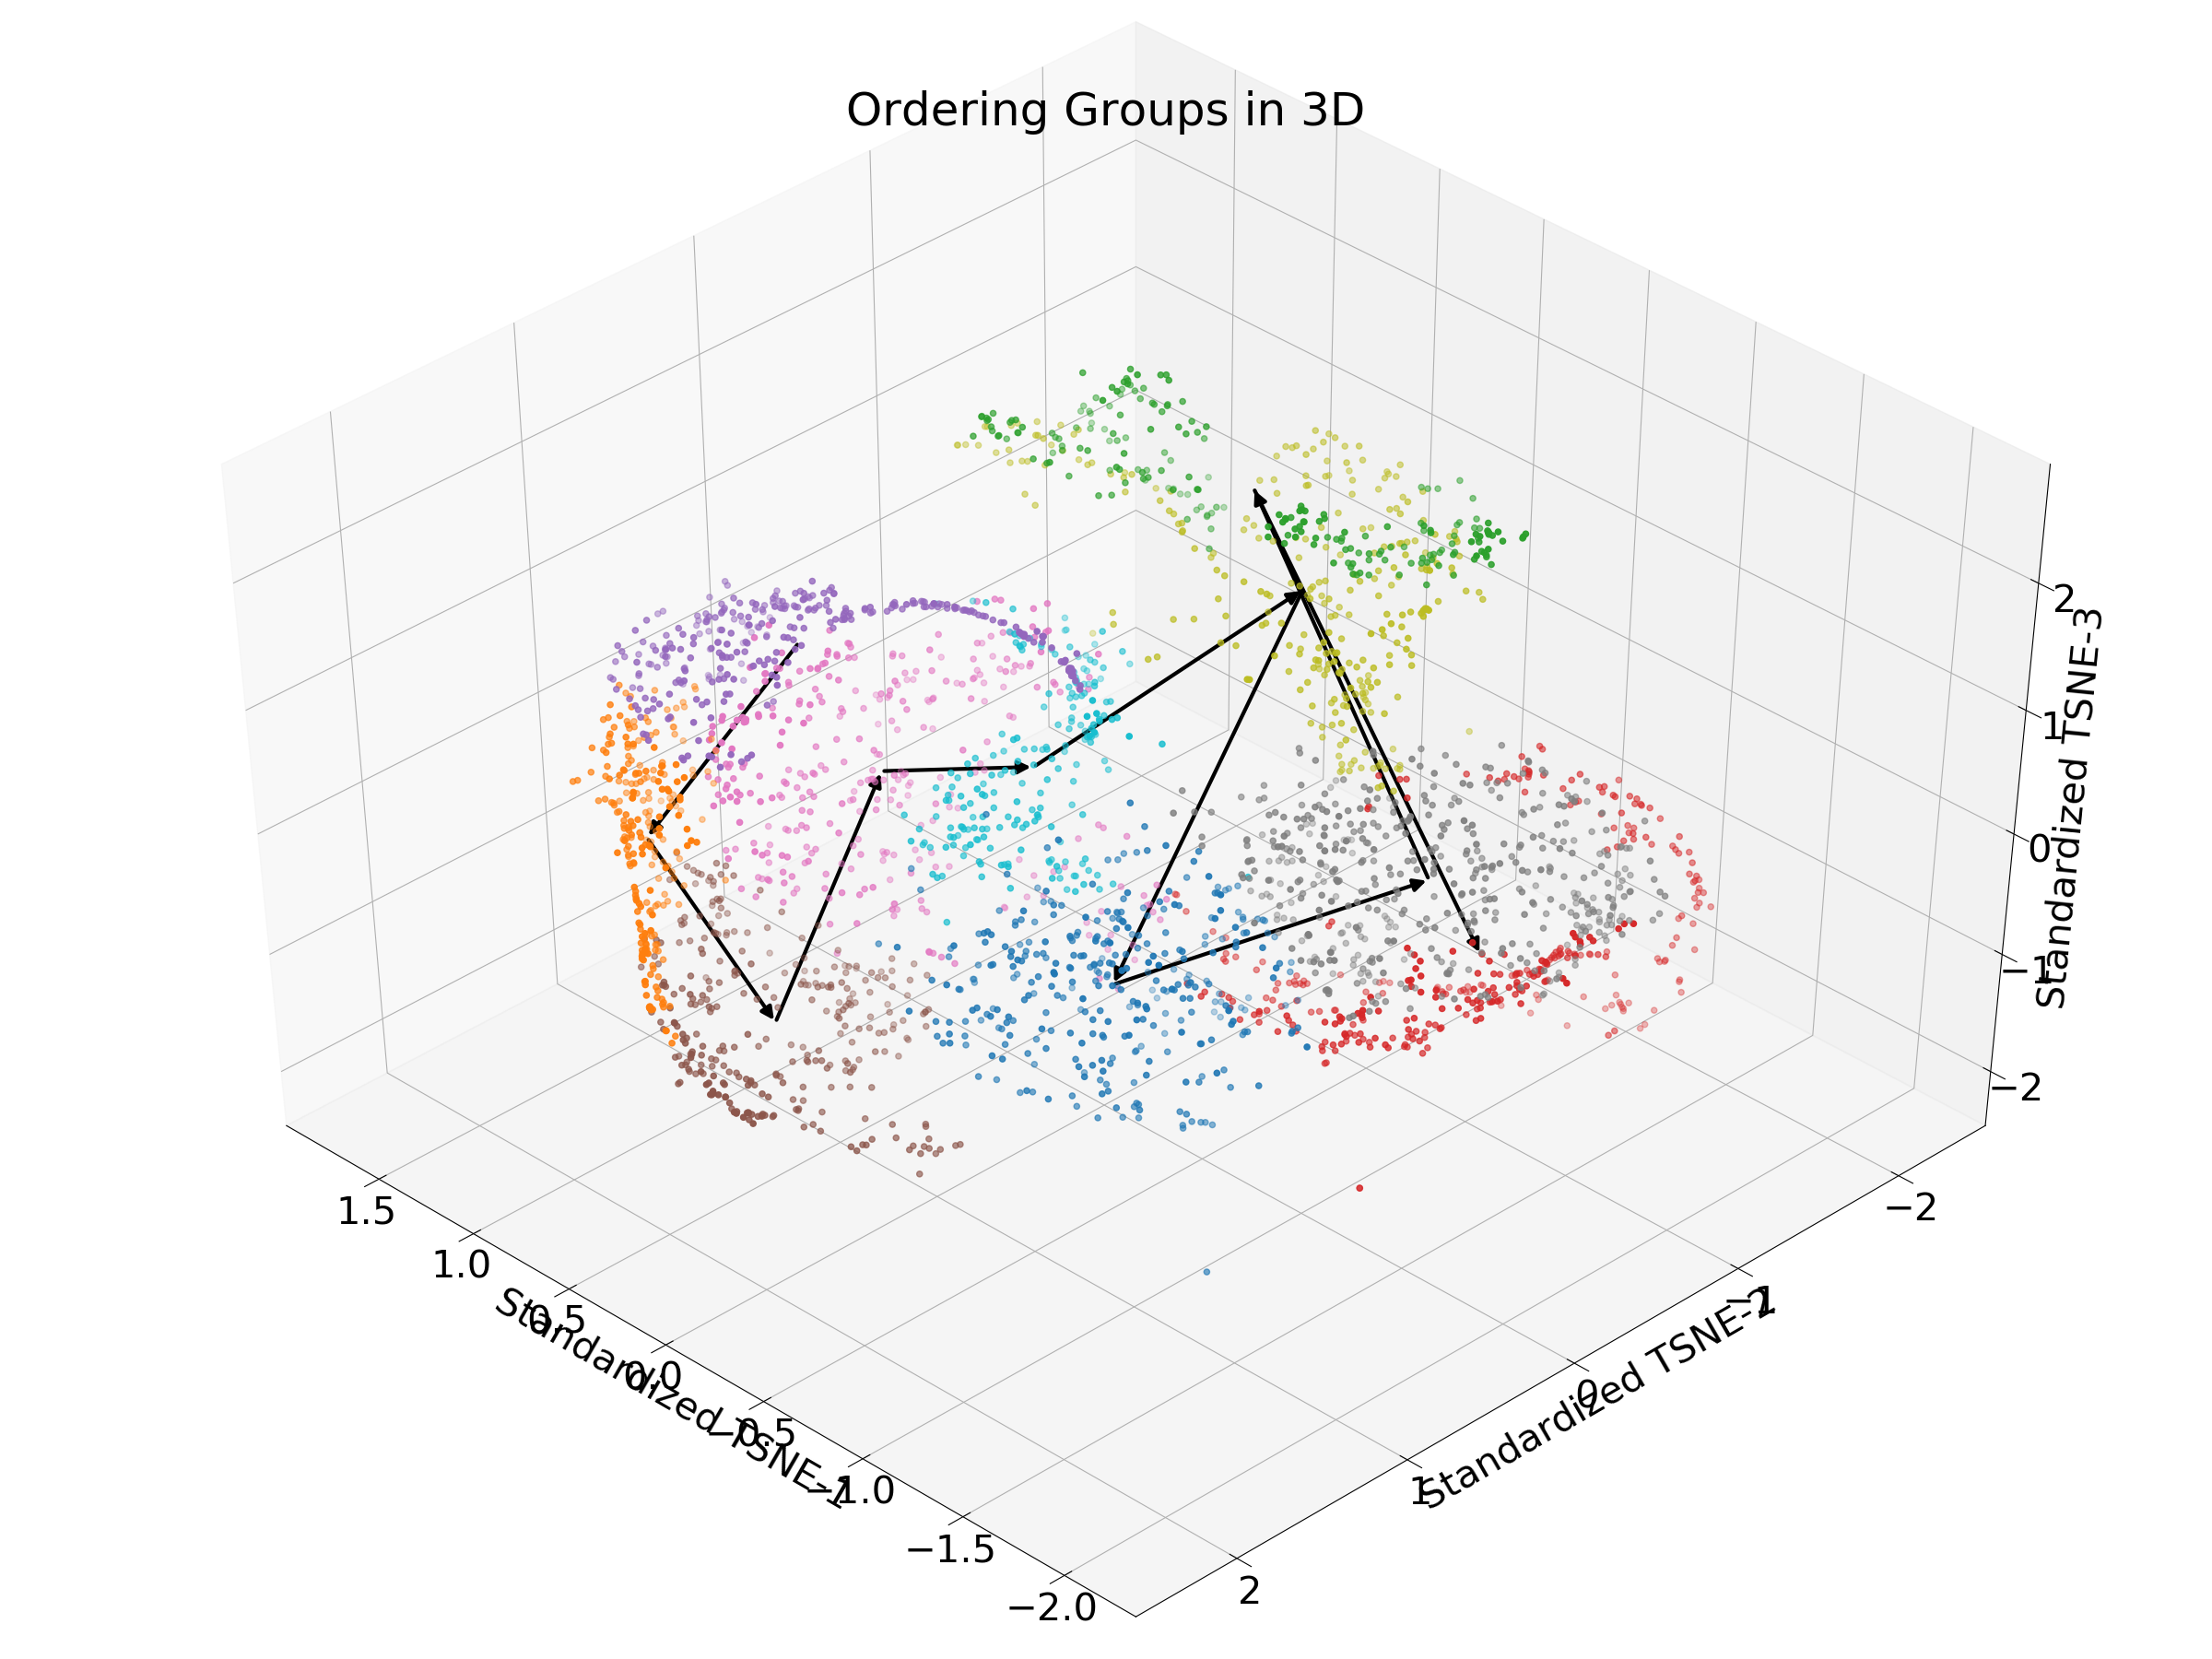
\includegraphics[height=5cm]{figures/Pseudotime/12Gene/3.png}
                            &
                            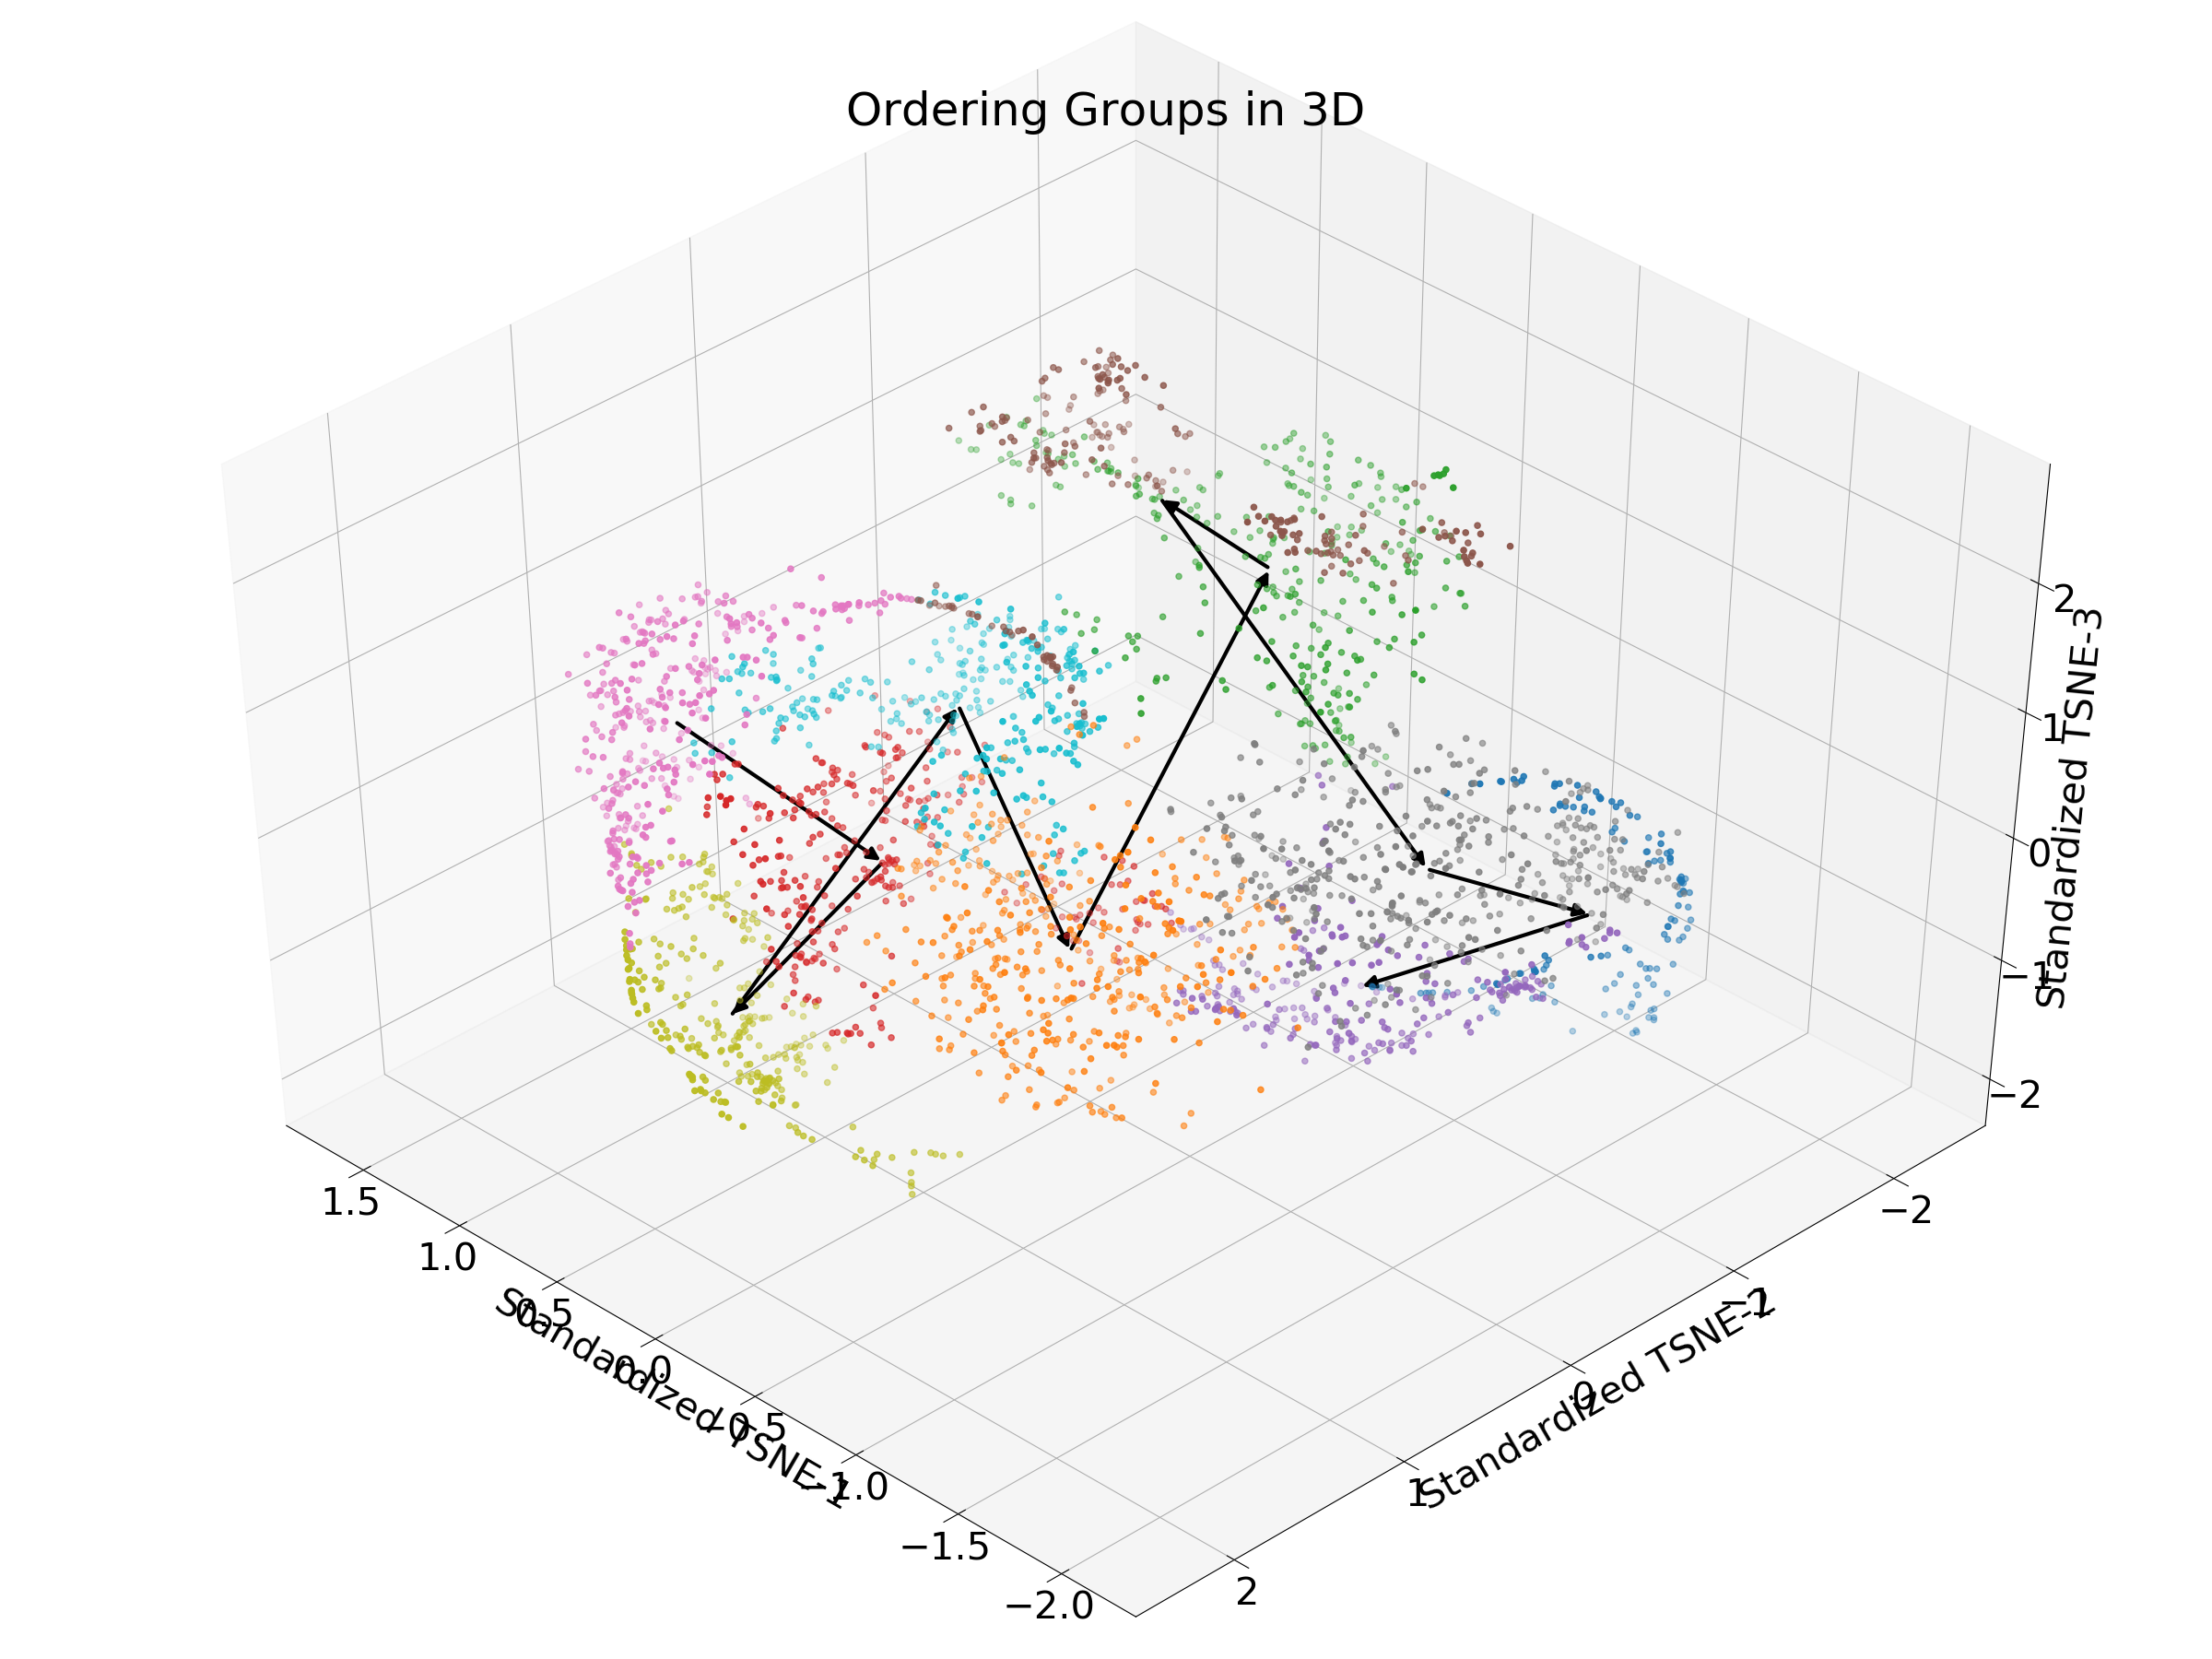
\includegraphics[height=5cm]{figures/Pseudotime/12Gene/4.png}
                            \\
                            
                            \mbox{(c) NS\_SW3} & \mbox{(d) NS\_SW4} \\
                        \end{array}$
                    \end{center}
                    \caption{Pseudo-time Plot with 12 Marker Genes}
                    \label{fig:time12gene}
                \end{figure}
            
            \subsubsection{65 Genes}
                The pseudo-time plots with 65 marker genes are in figure \ref{fig:time65gene}.
                \begin{figure}[hbp]
                    \begin{center}
                        $\begin{array}{cc}
                            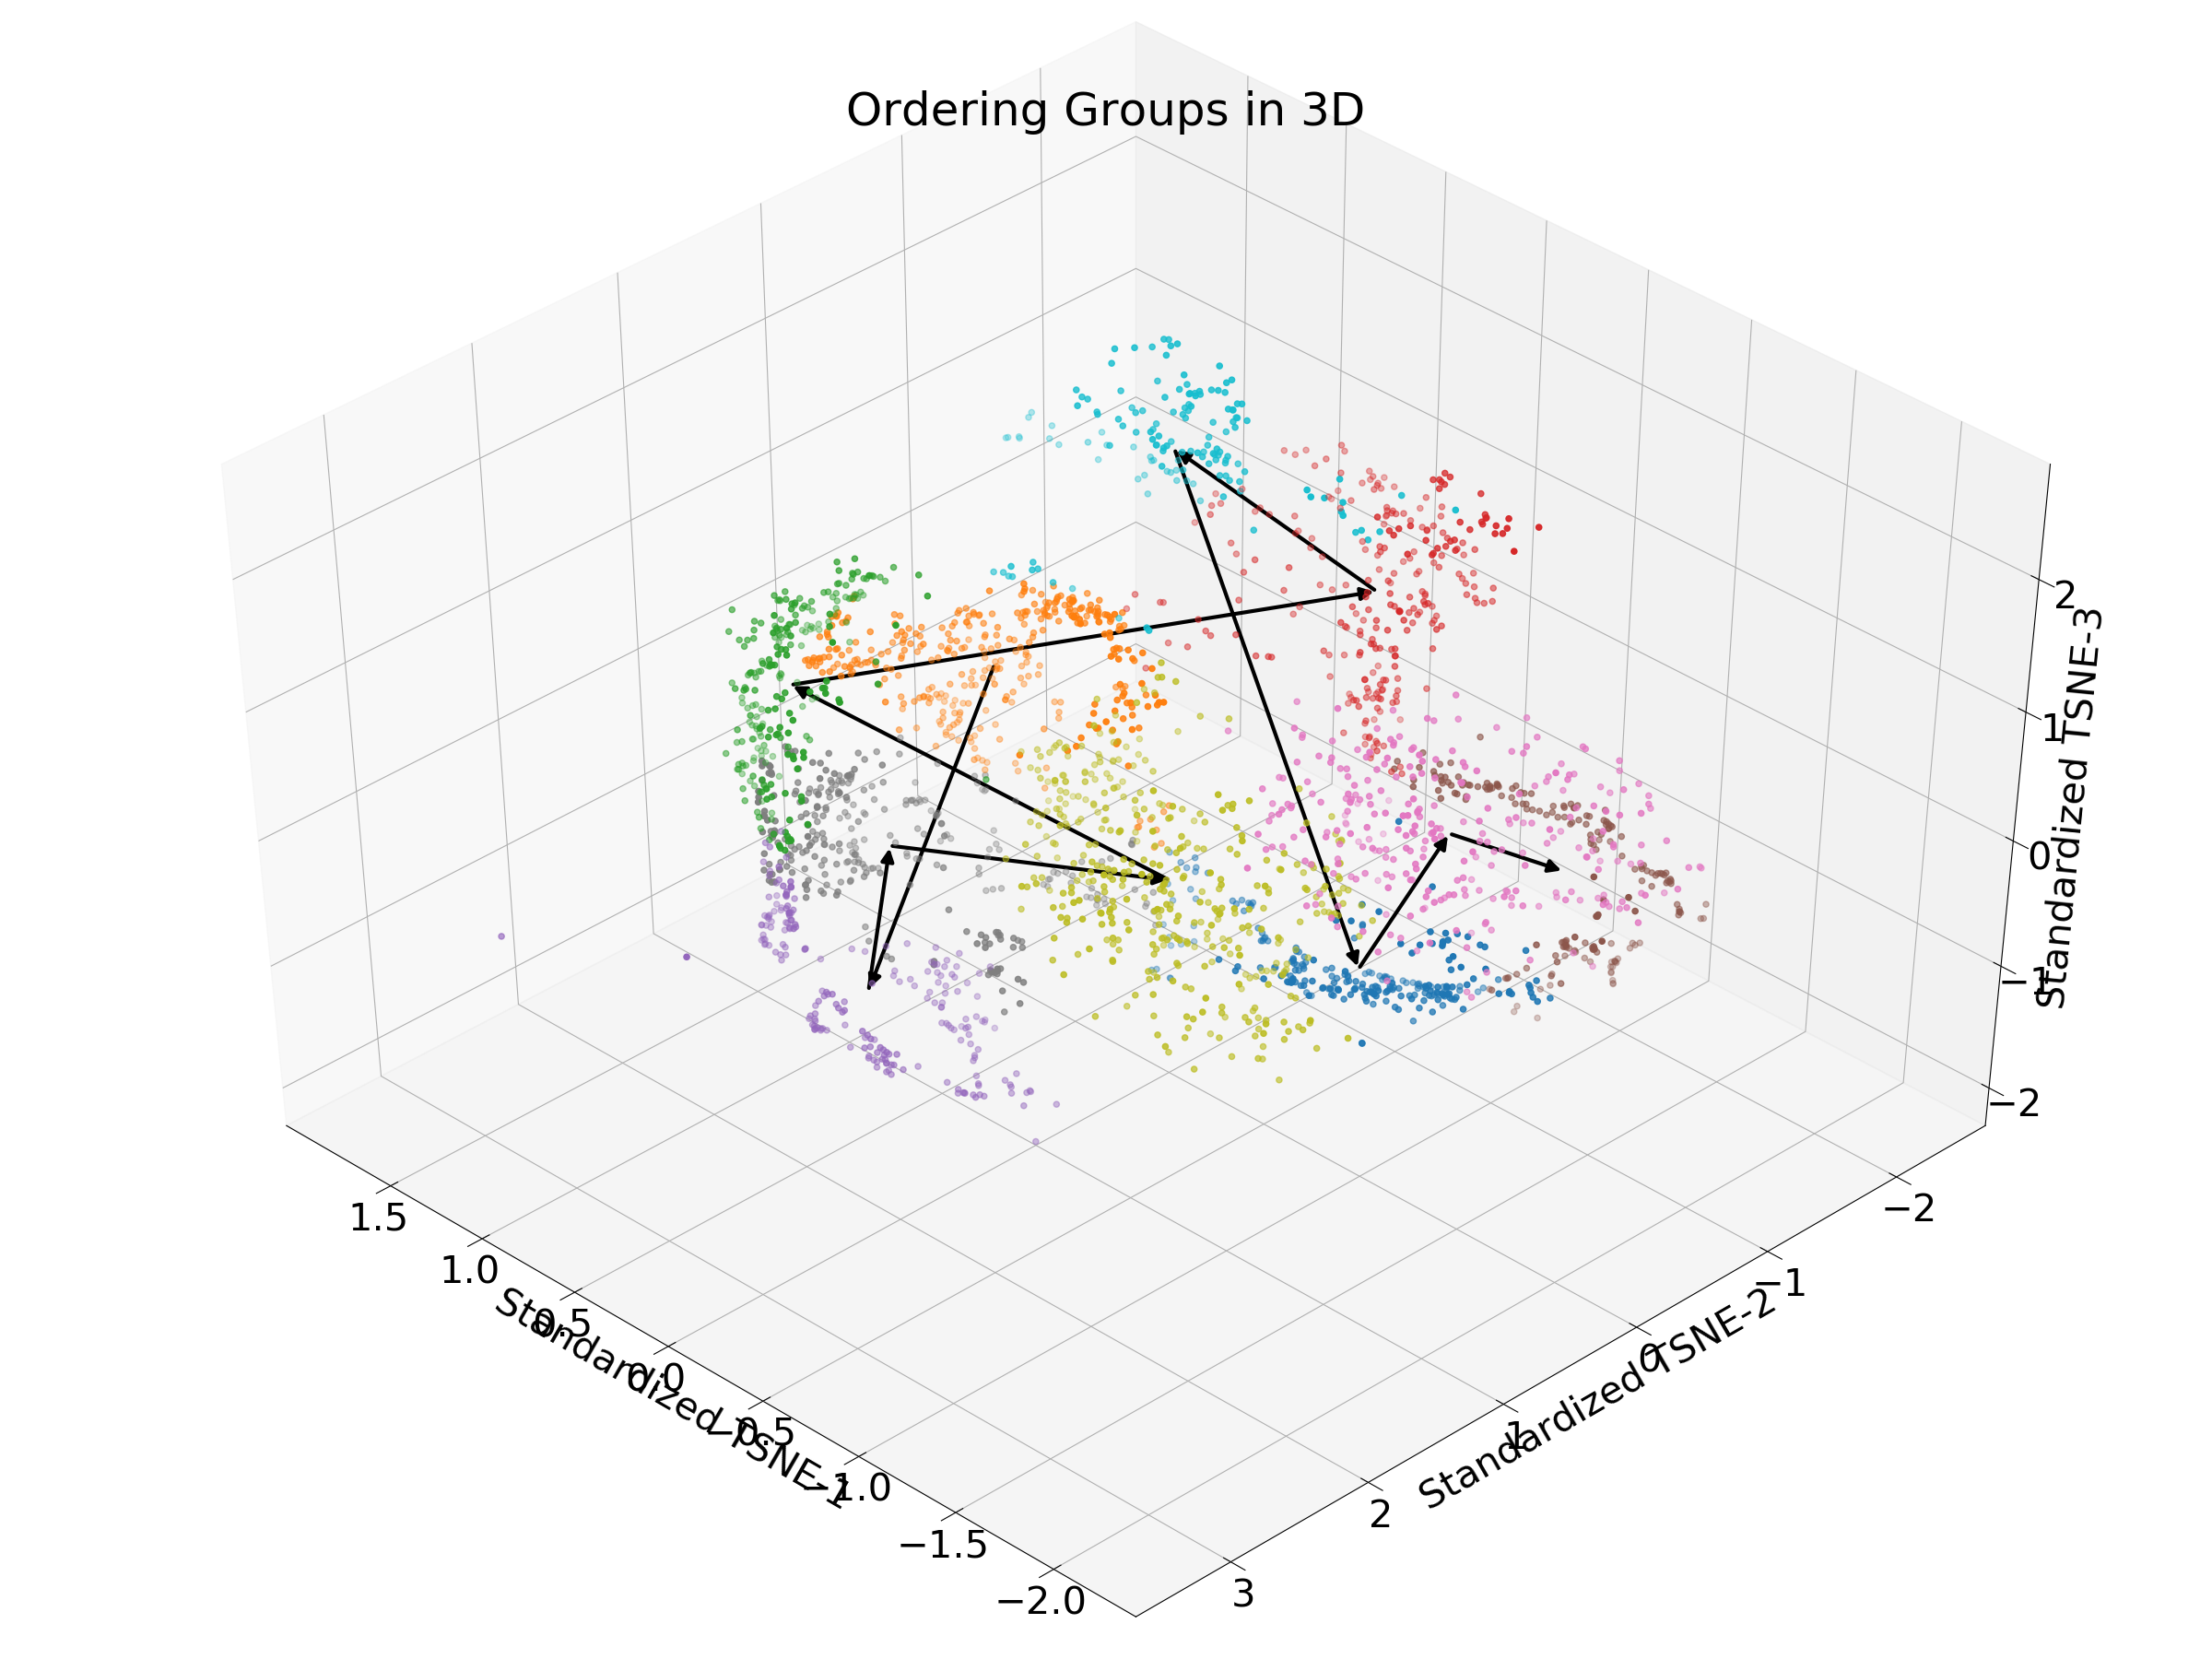
\includegraphics[height=5cm]{figures/Pseudotime/65Gene/1.png}
                            &
                            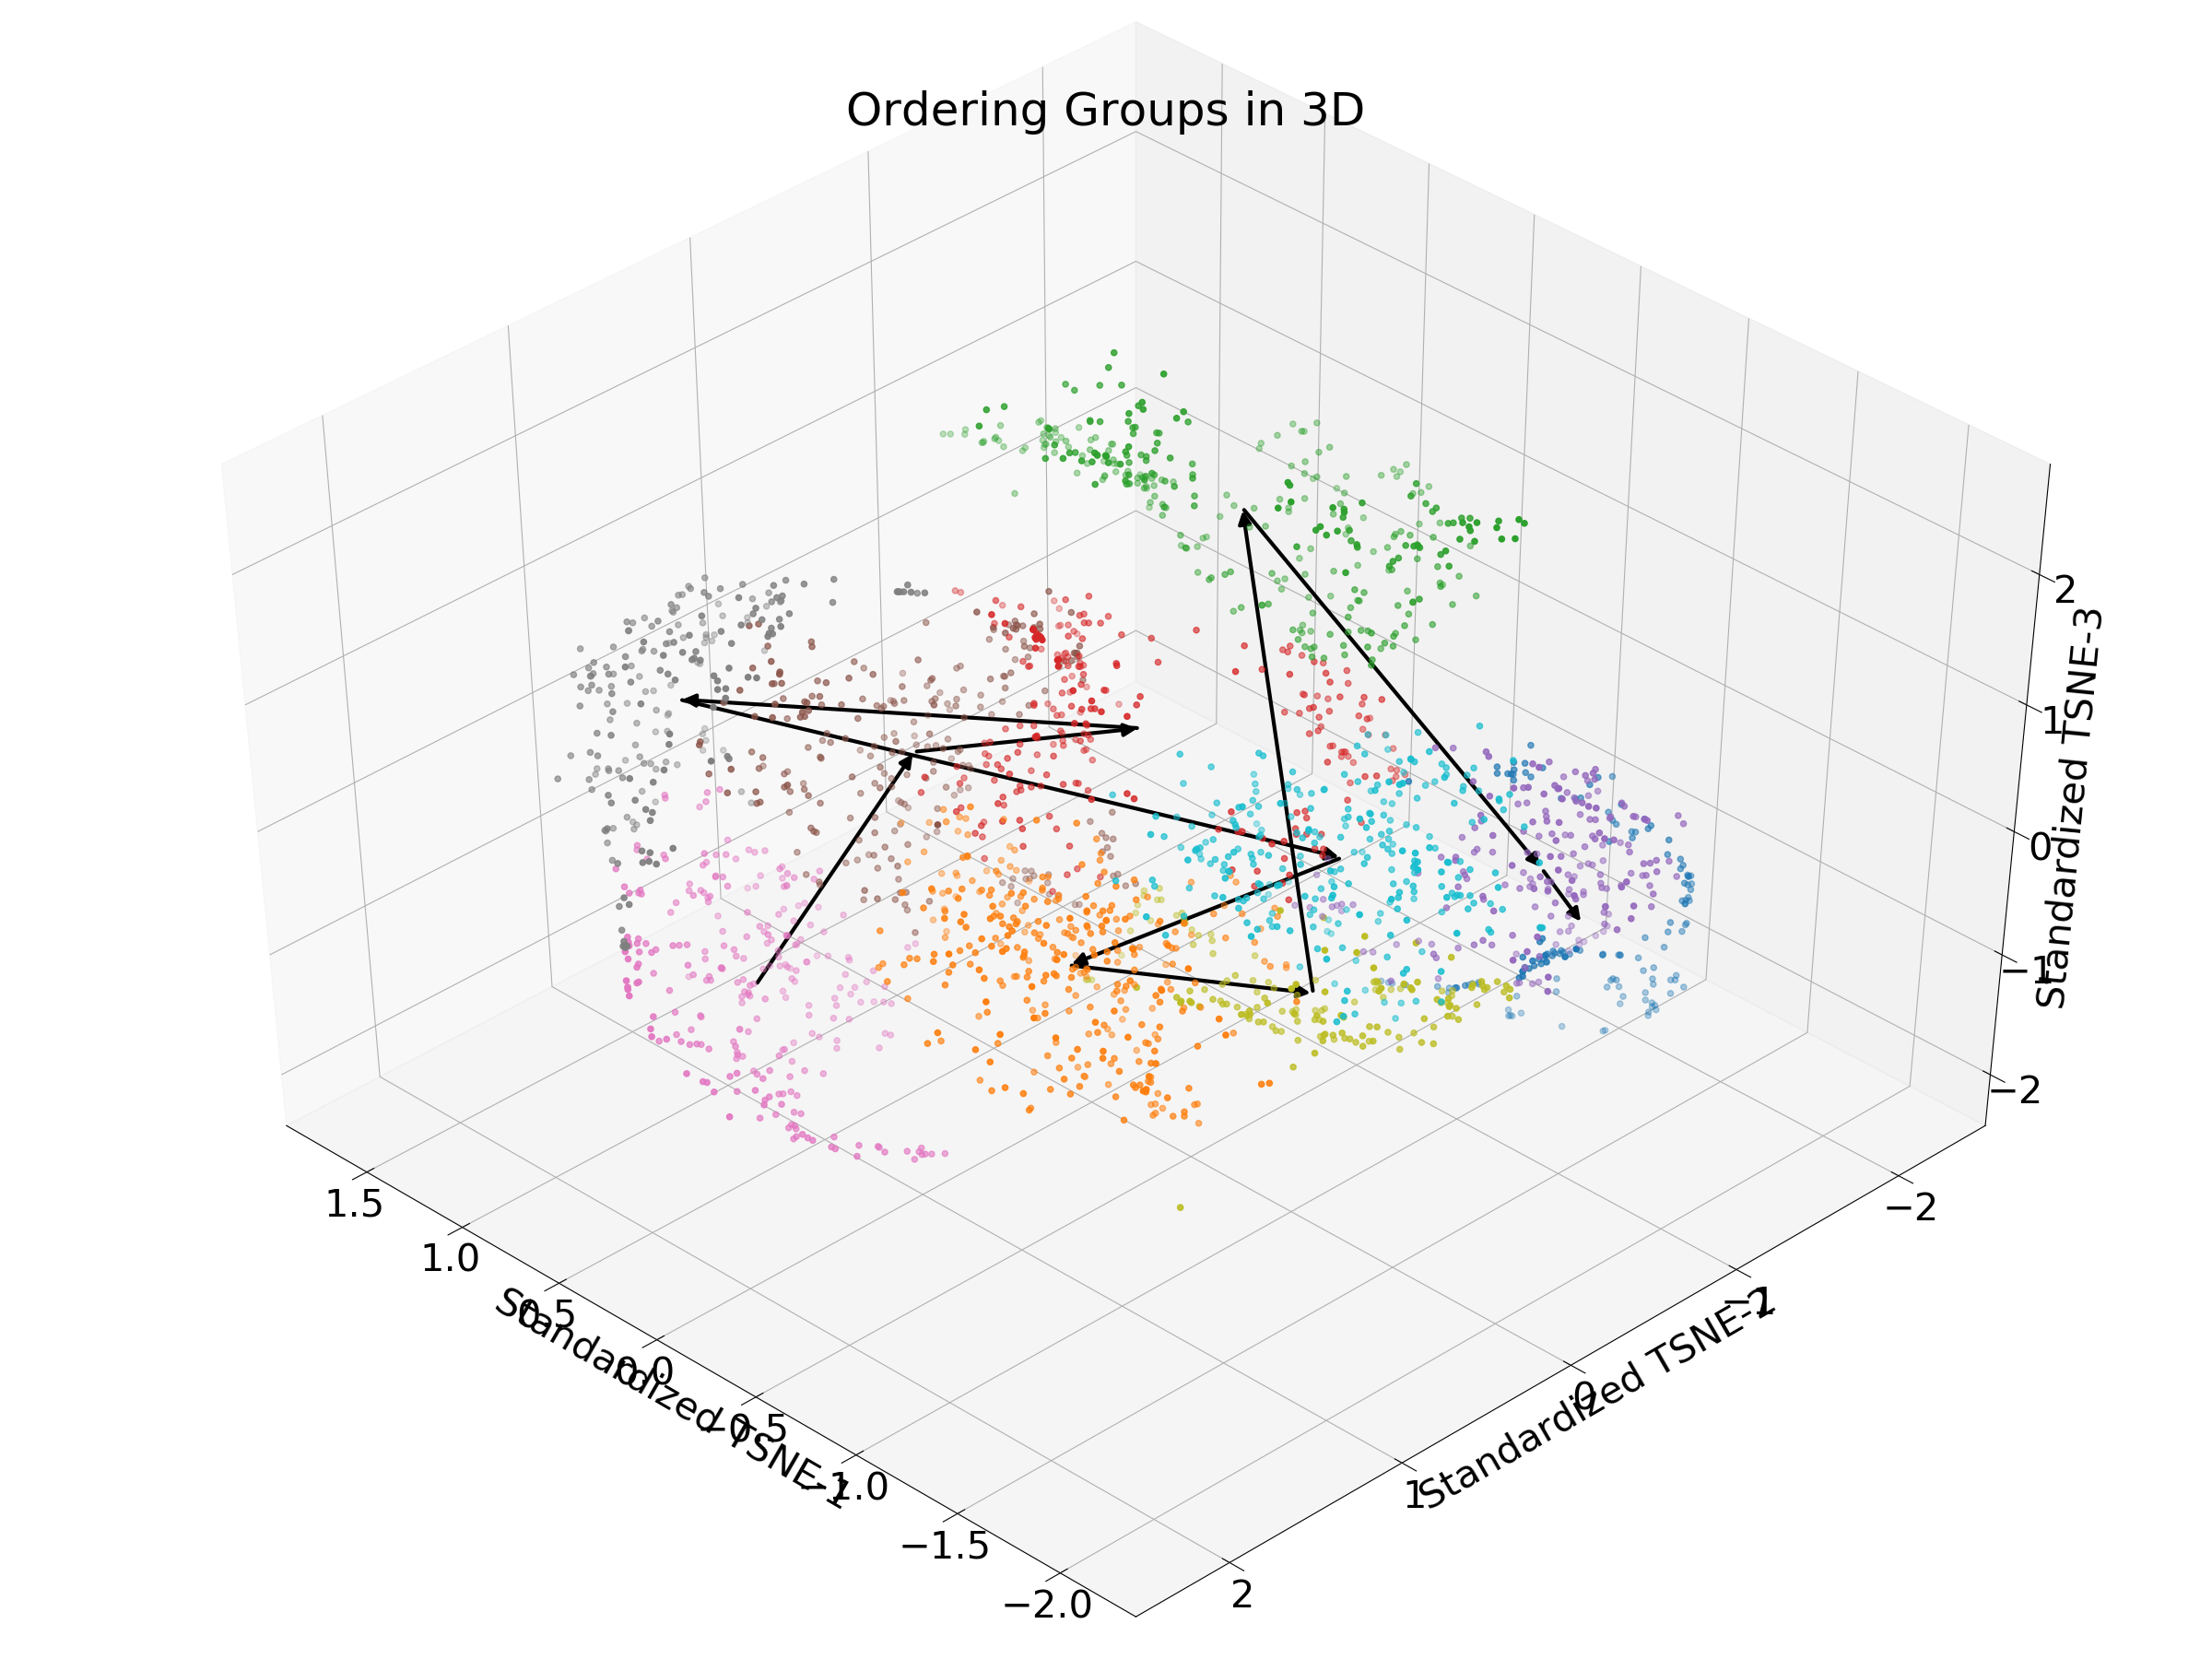
\includegraphics[height=5cm]{figures/Pseudotime/65Gene/2.png}\\
                            
                            \mbox{(a) NS\_SW1} & \mbox{(b) NS\_SW2} \\
                            
                            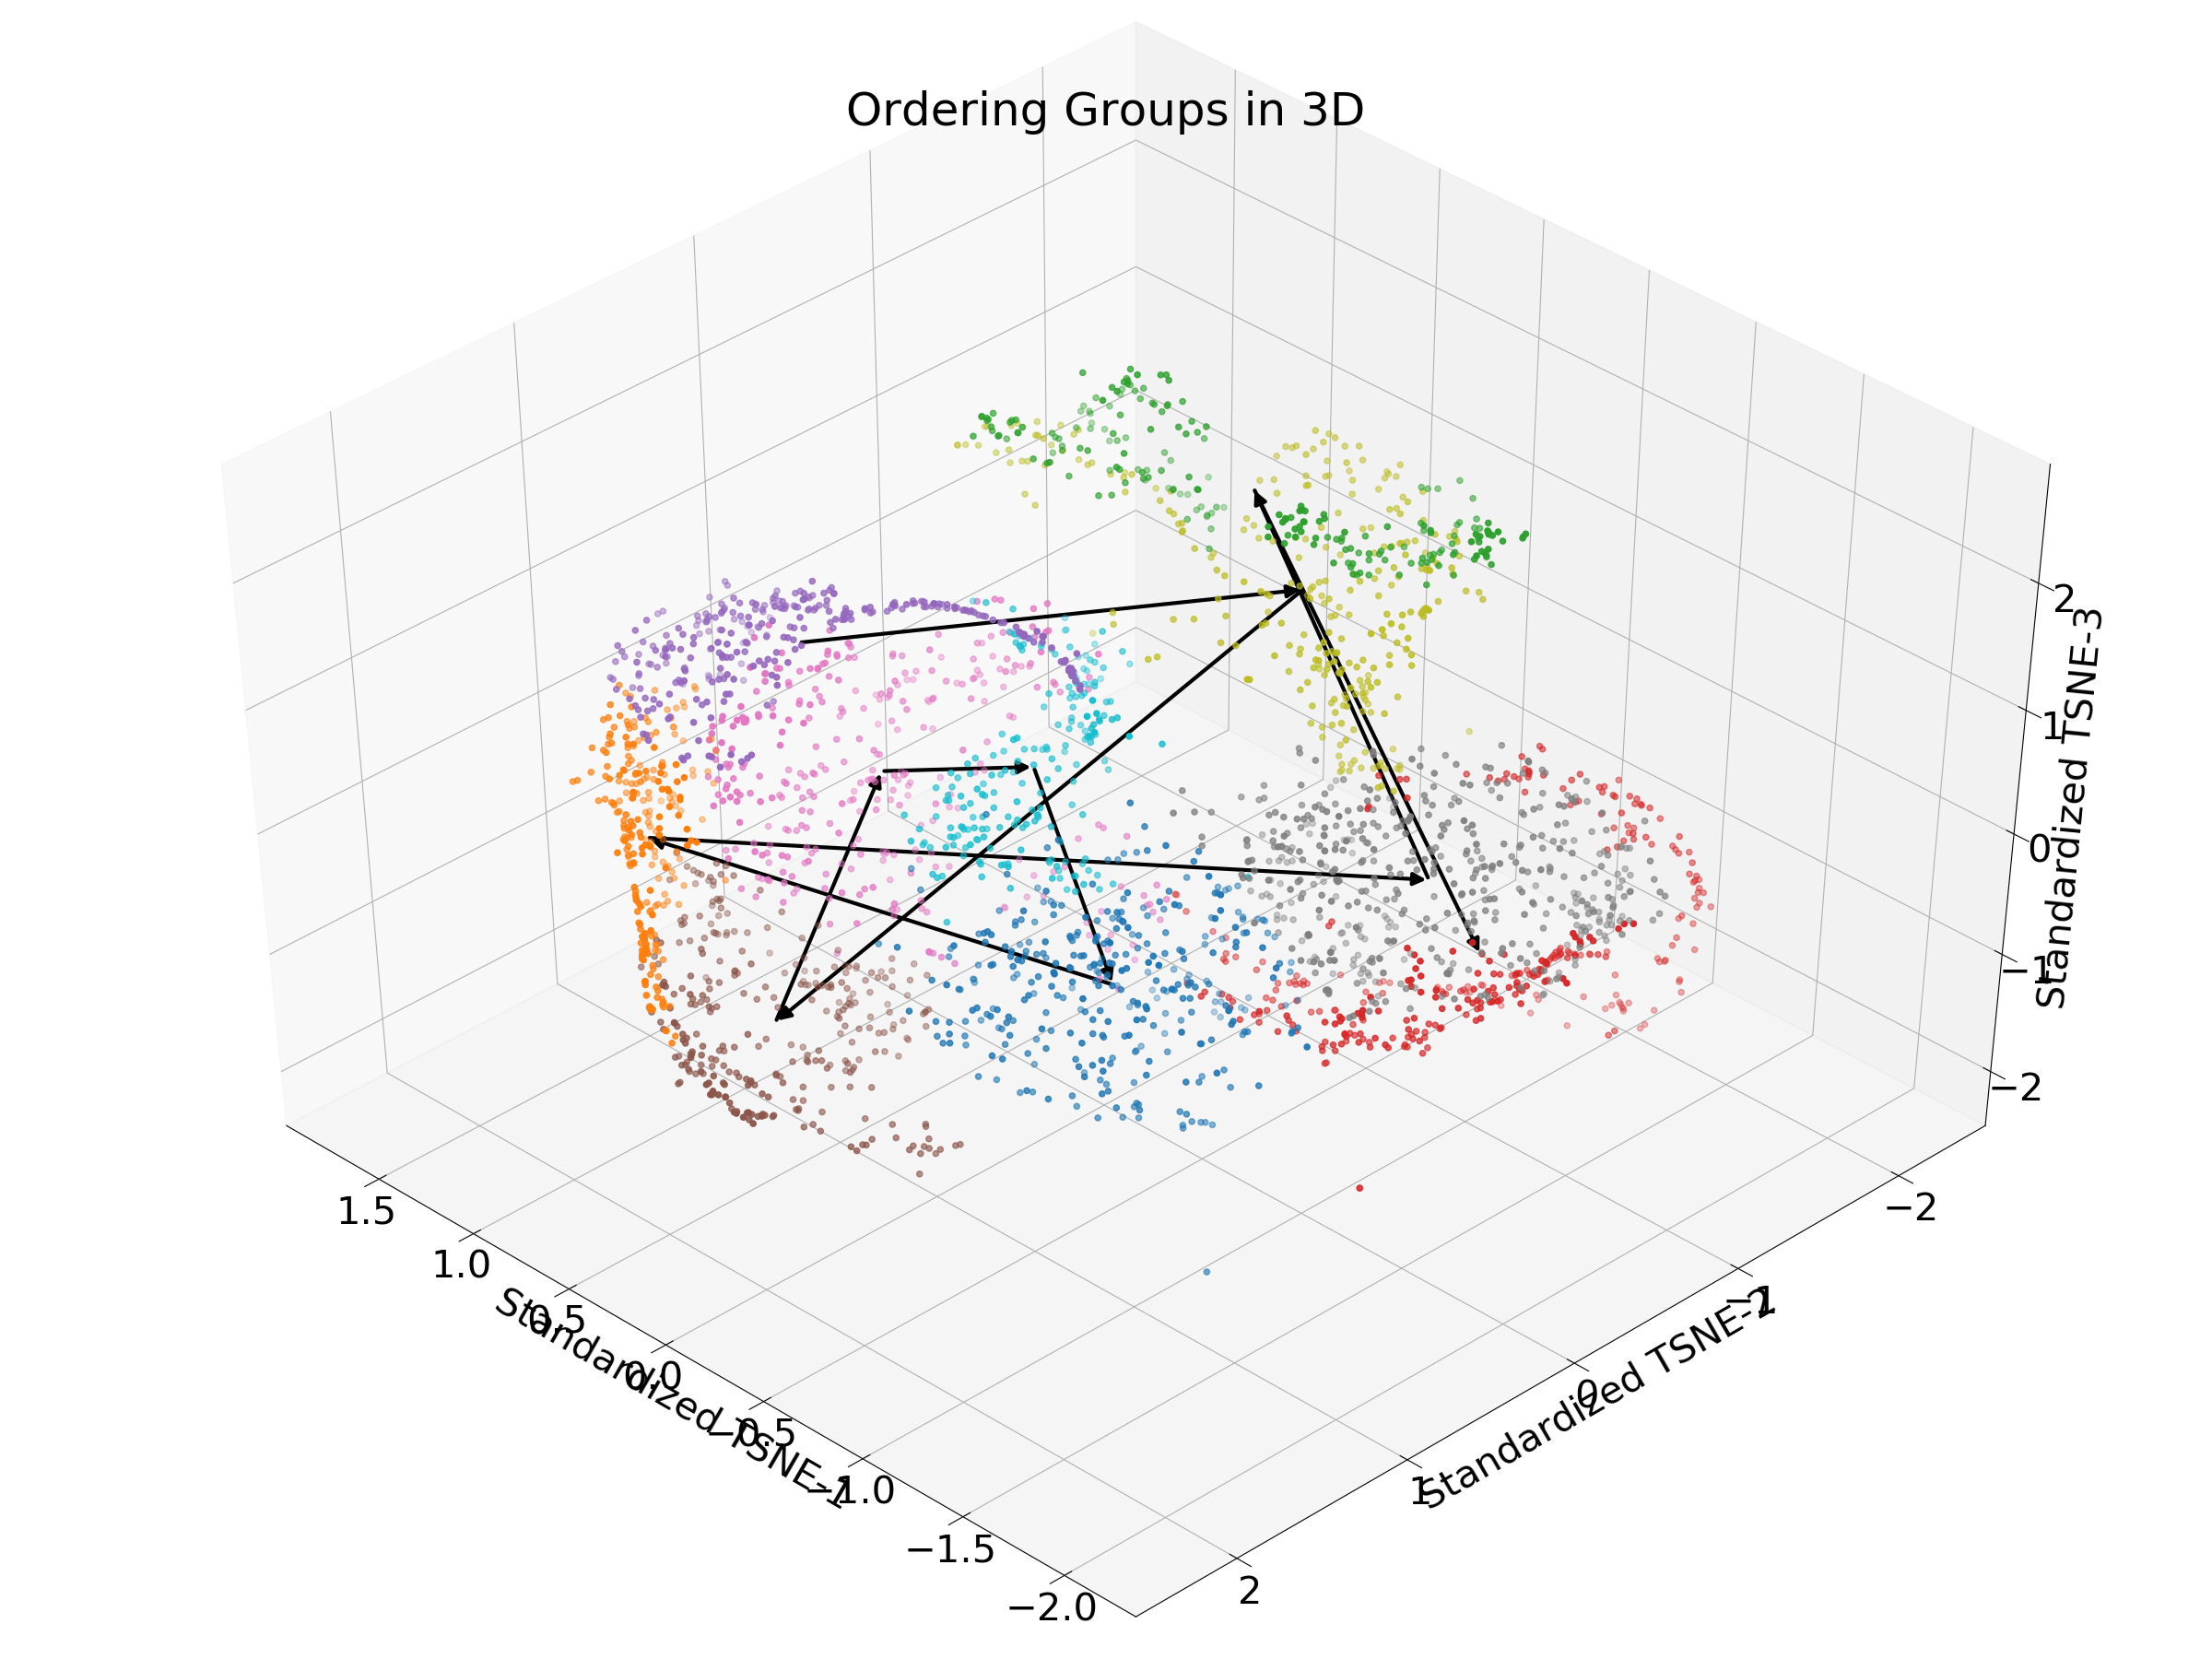
\includegraphics[height=5cm]{figures/Pseudotime/65Gene/3.png}
                            &
                            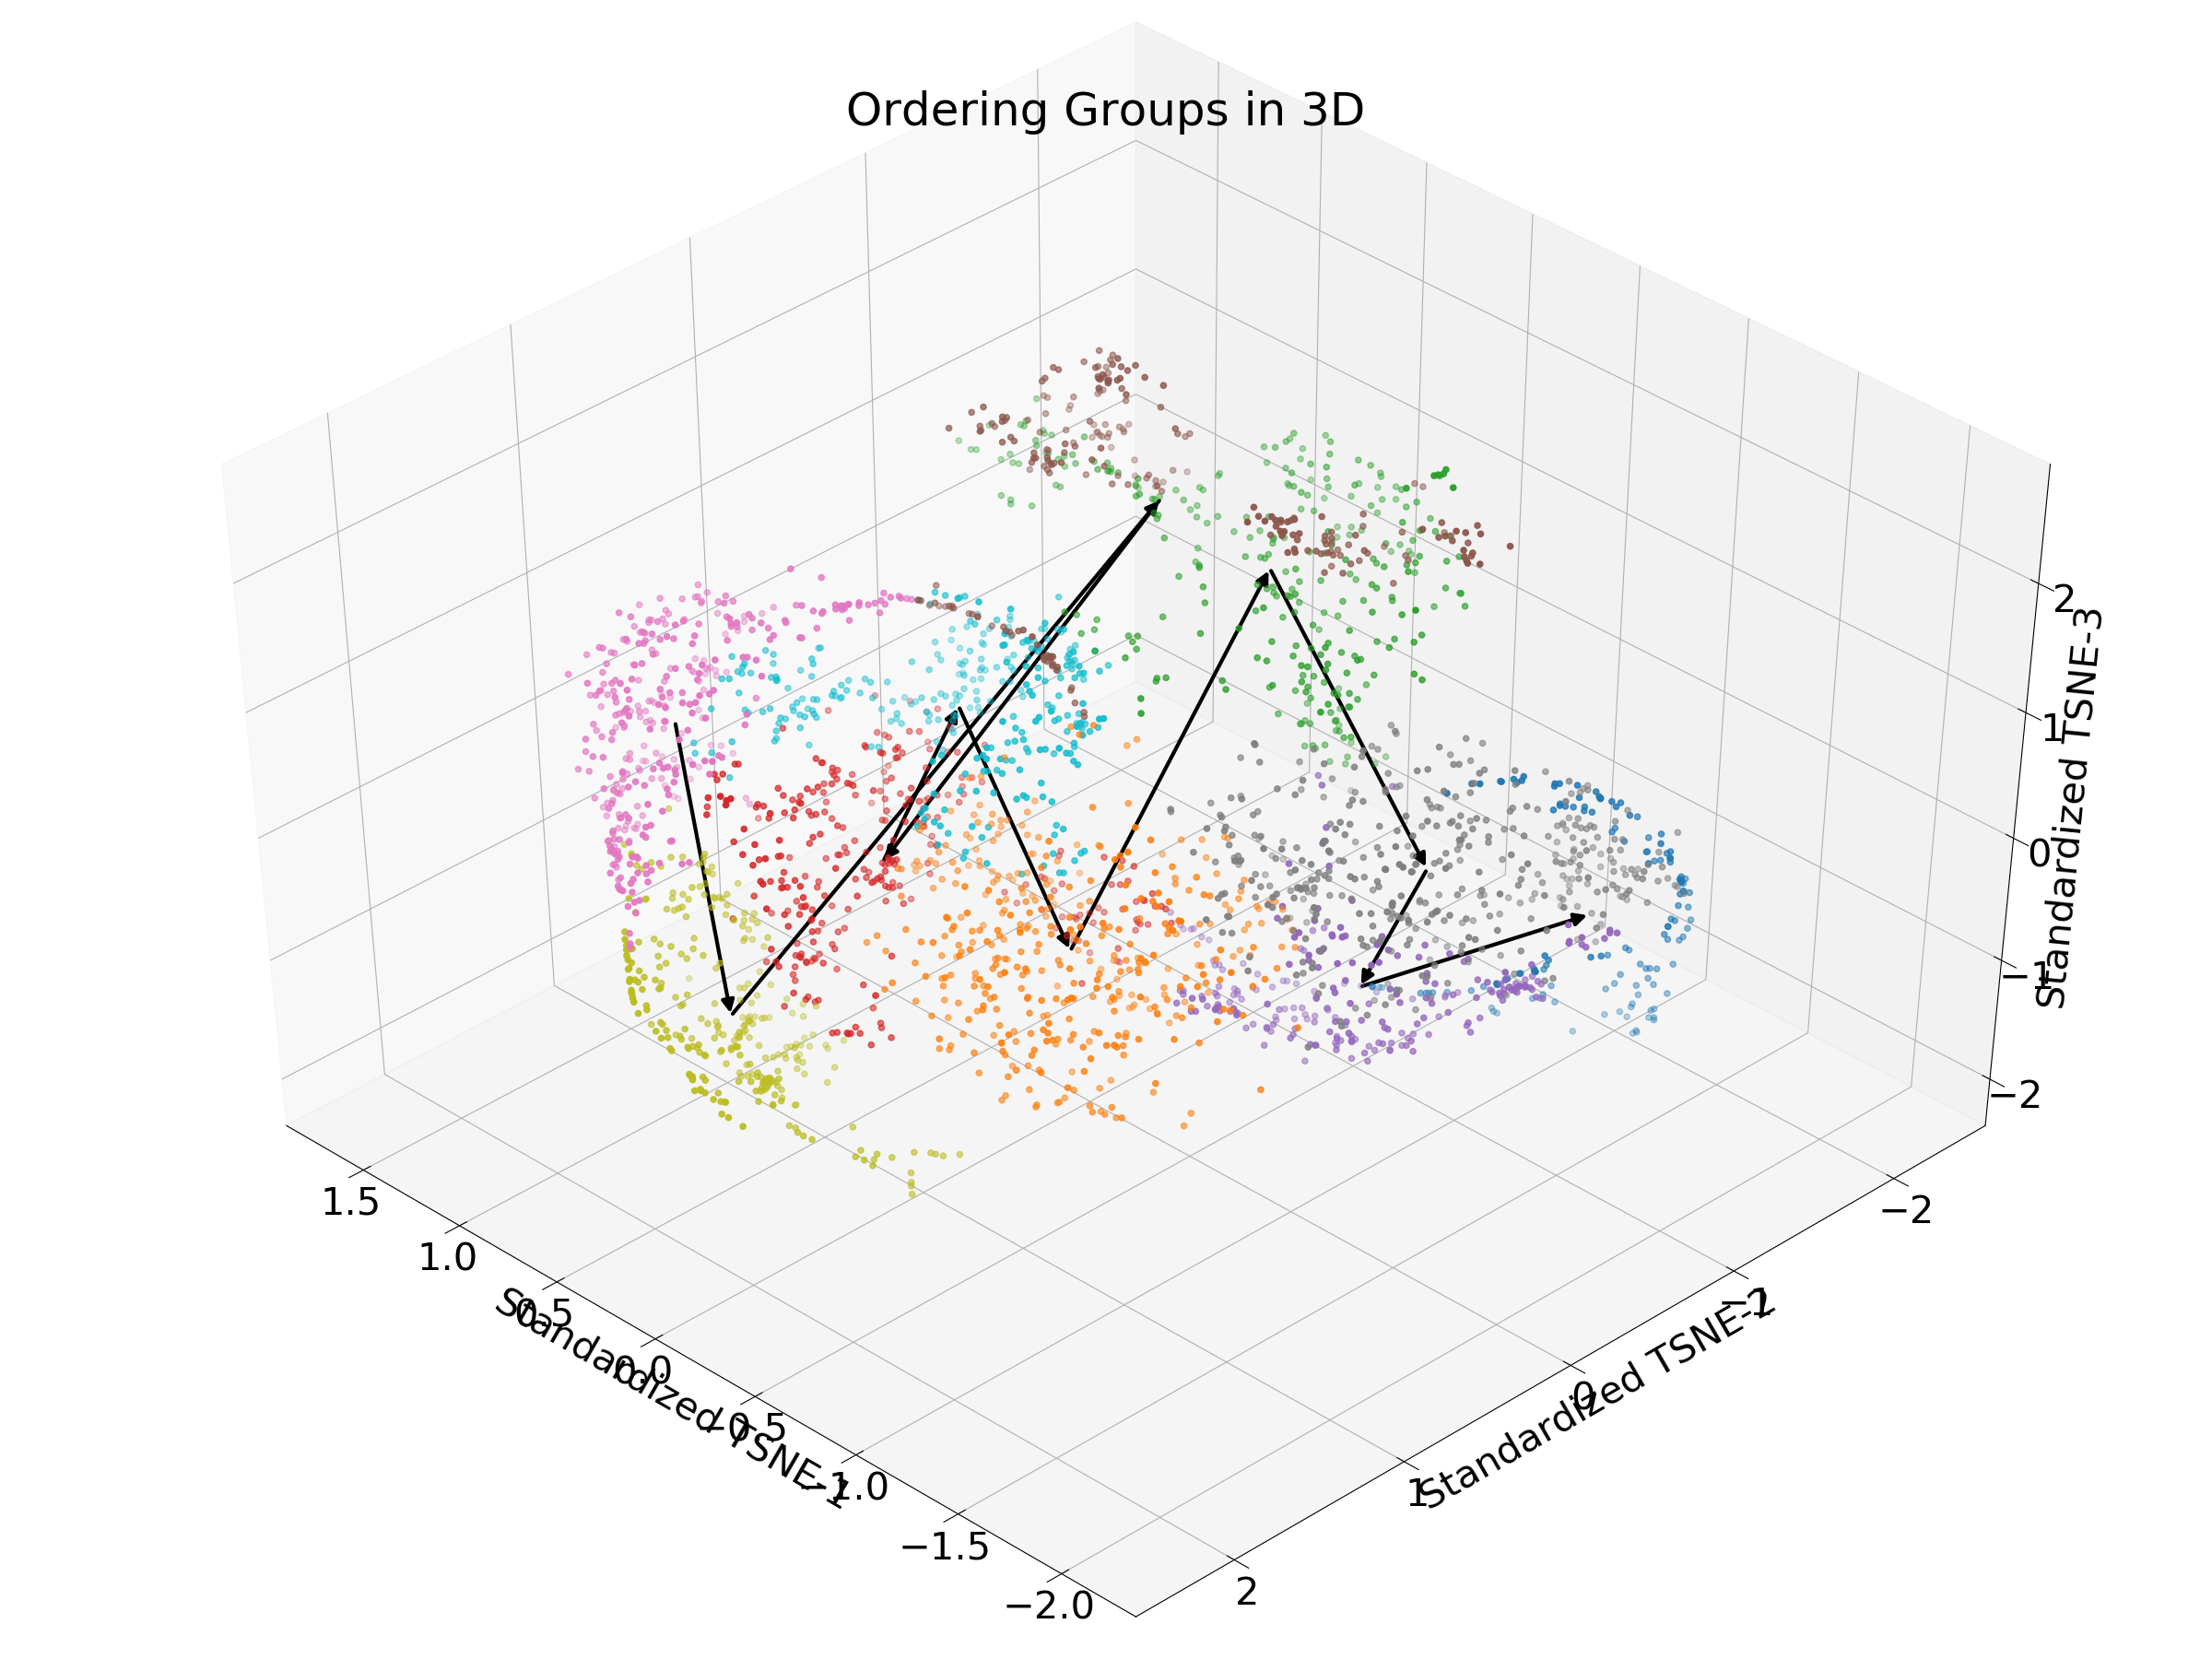
\includegraphics[height=5cm]{figures/Pseudotime/65Gene/4.png}\\
                            
                            \mbox{(c) NS\_SW3} & \mbox{(d) NS\_SW4} \\
                        \end{array}$
                    \end{center}
                    \caption{Pseudo-time Plot with 65 Marker Genes}
                    \label{fig:time65gene}
                \end{figure}
            
            \subsubsection{Top 10 Gene}
                The heatmap plots with the 10 genes which have highest gene expression are in figure \ref{fig:time10gene}.
                \begin{figure}[hbp]
                    \begin{center}
                        $\begin{array}{cc}
                            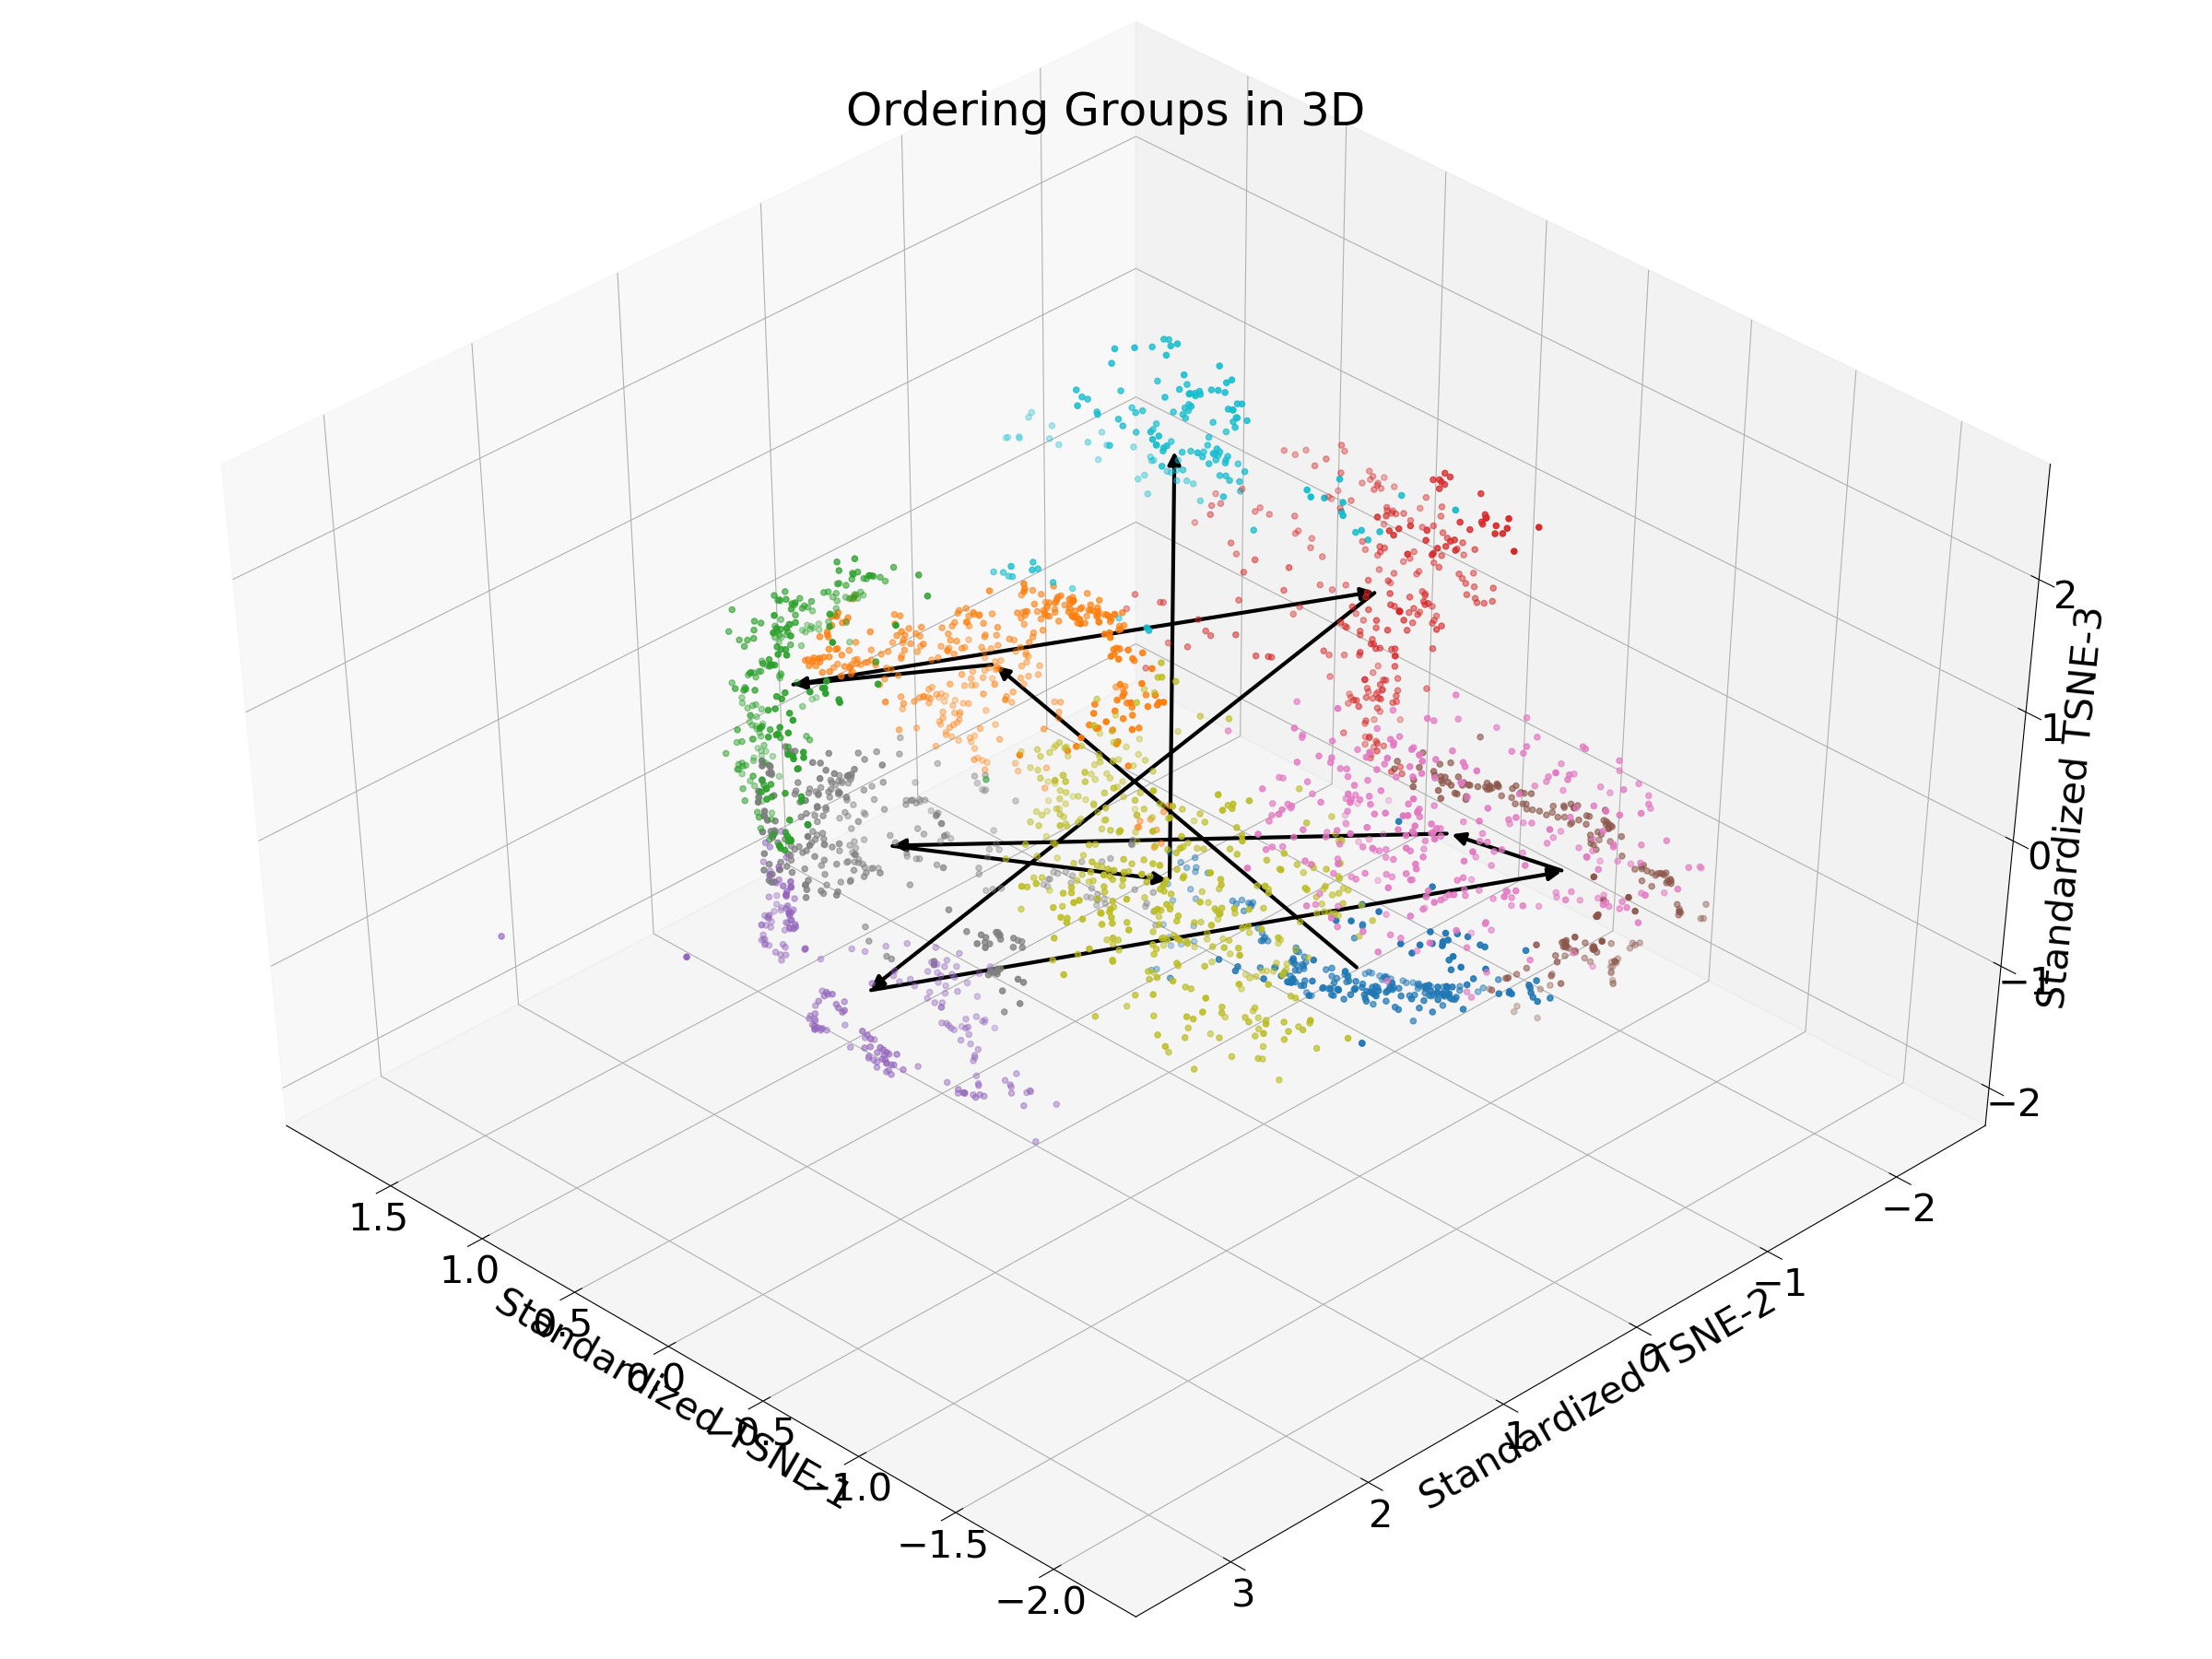
\includegraphics[height=5cm]{figures/Pseudotime/Top10/1.png}
                            &
                            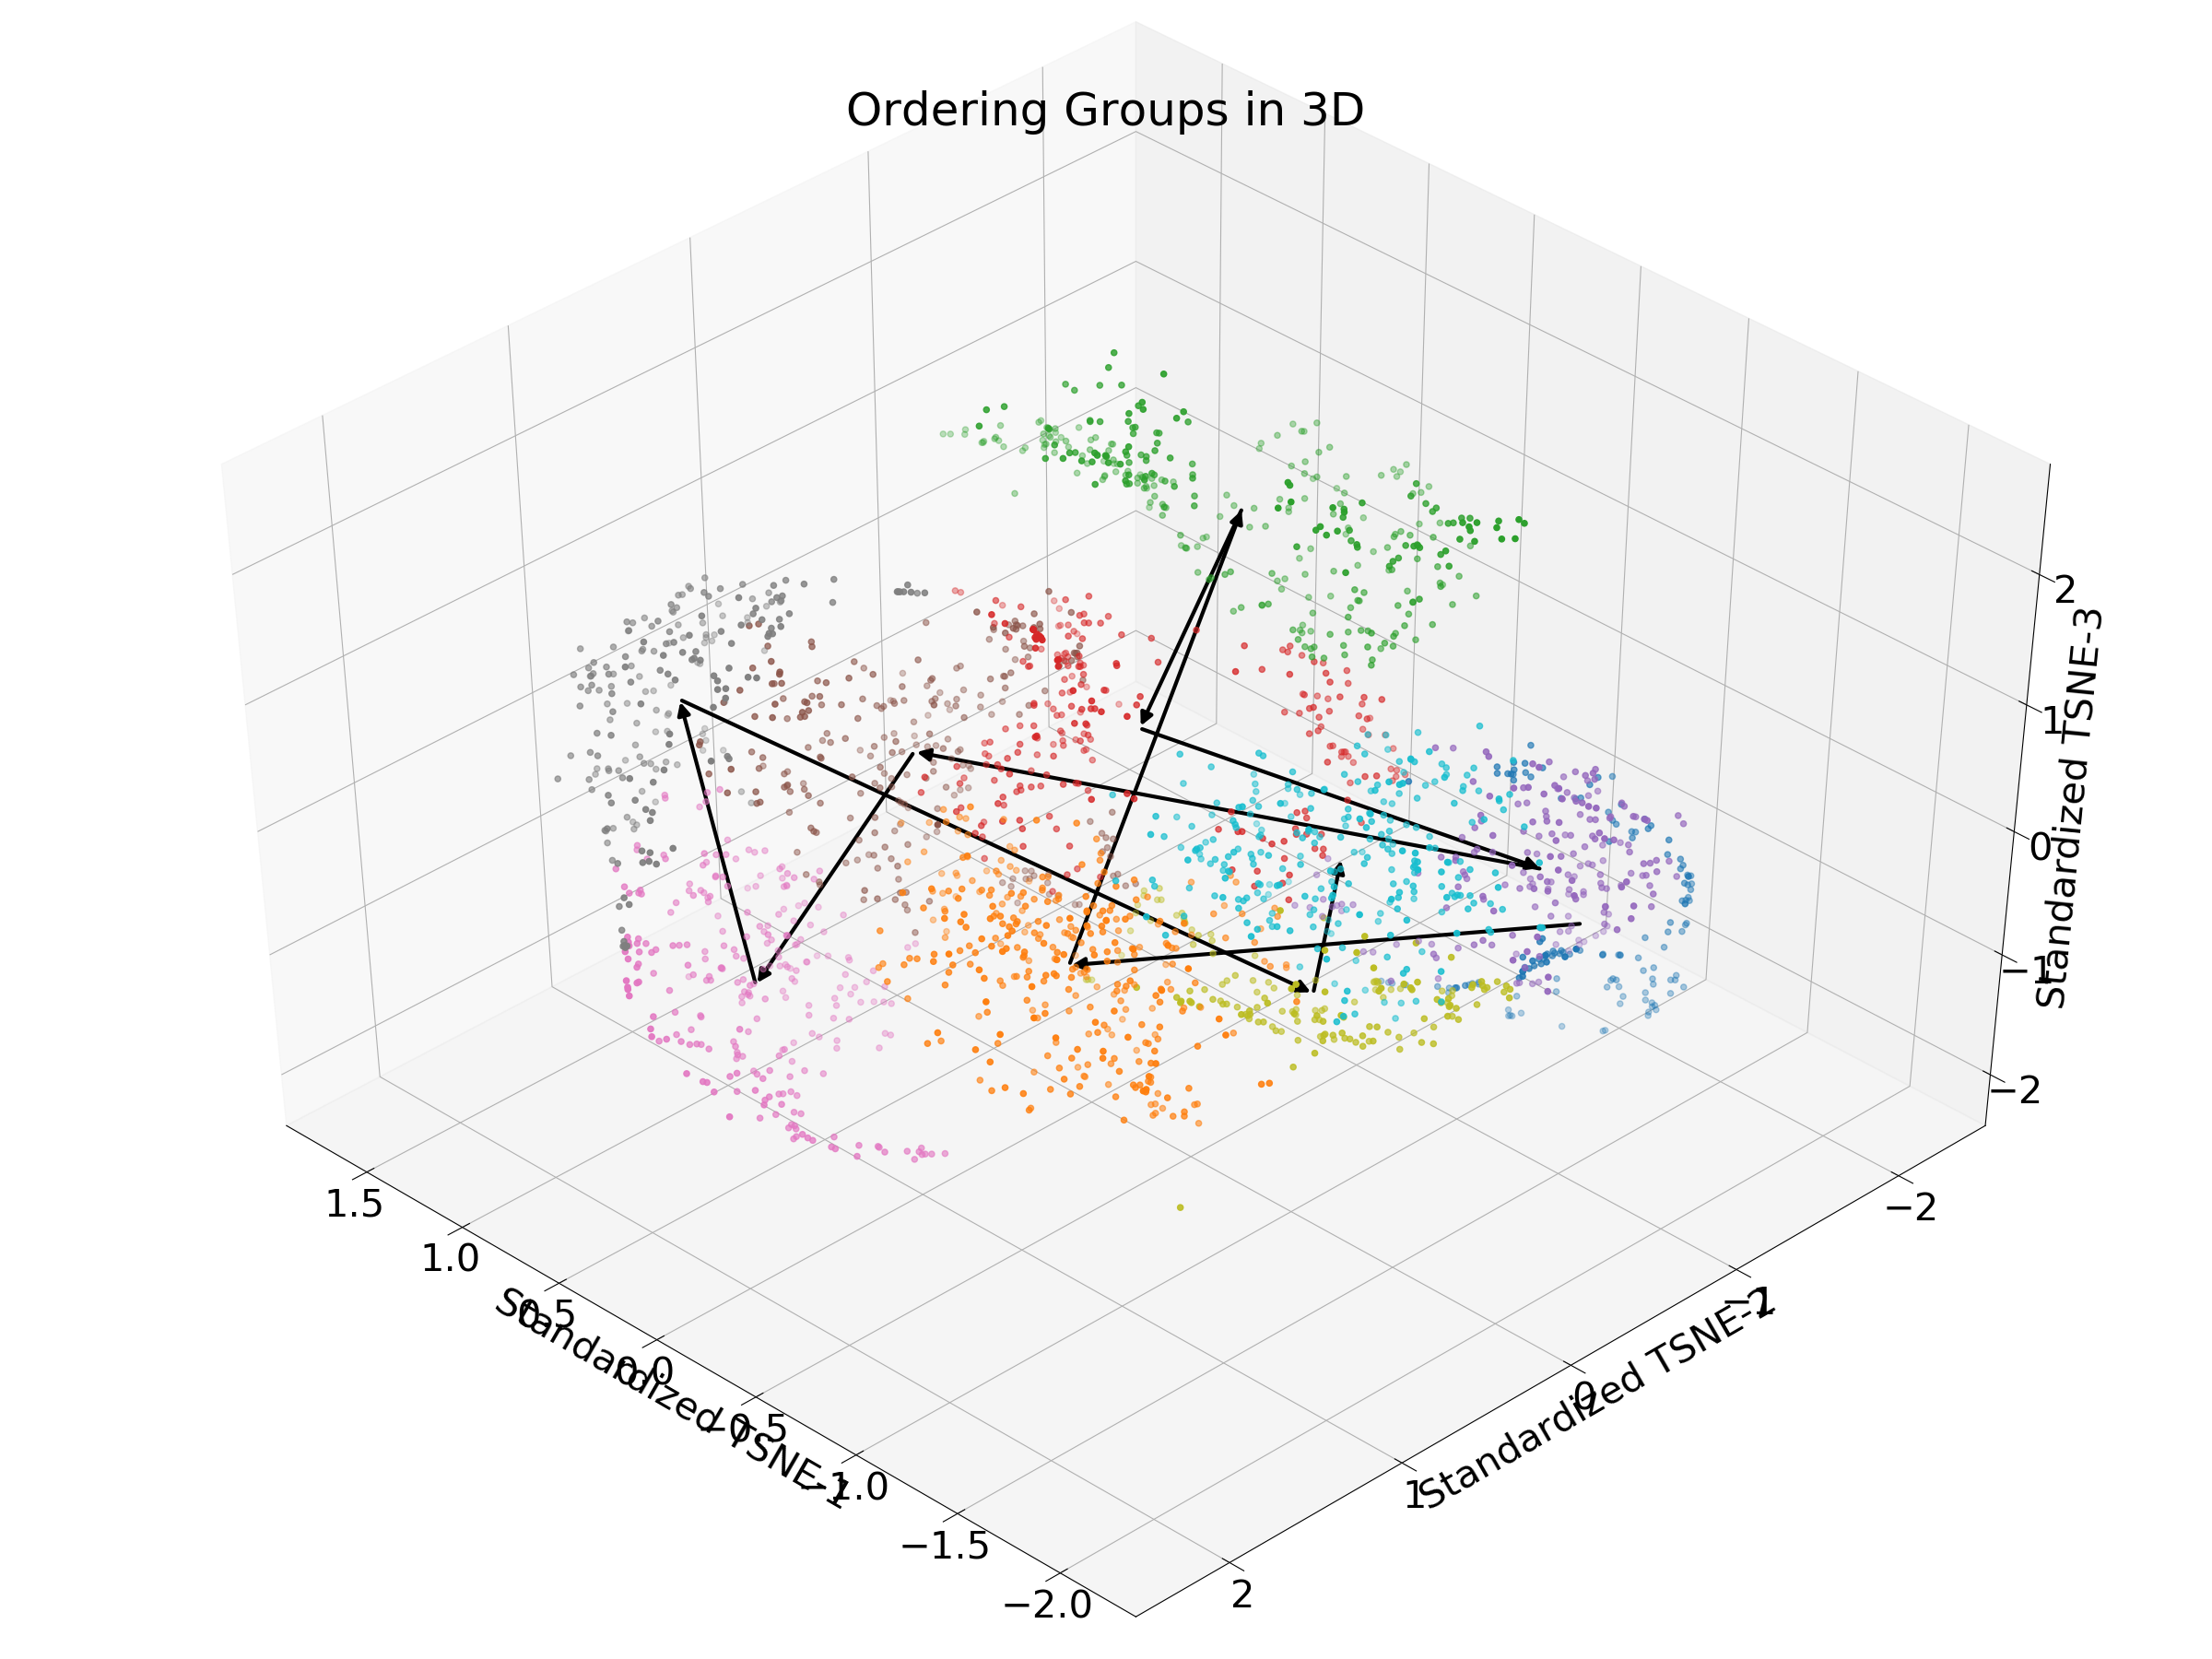
\includegraphics[height=5cm]{figures/Pseudotime/Top10/2.png}
                            \\
                            
                            \mbox{(a) NS\_SW1} & \mbox{(b) NS\_SW2} \\
                            
                            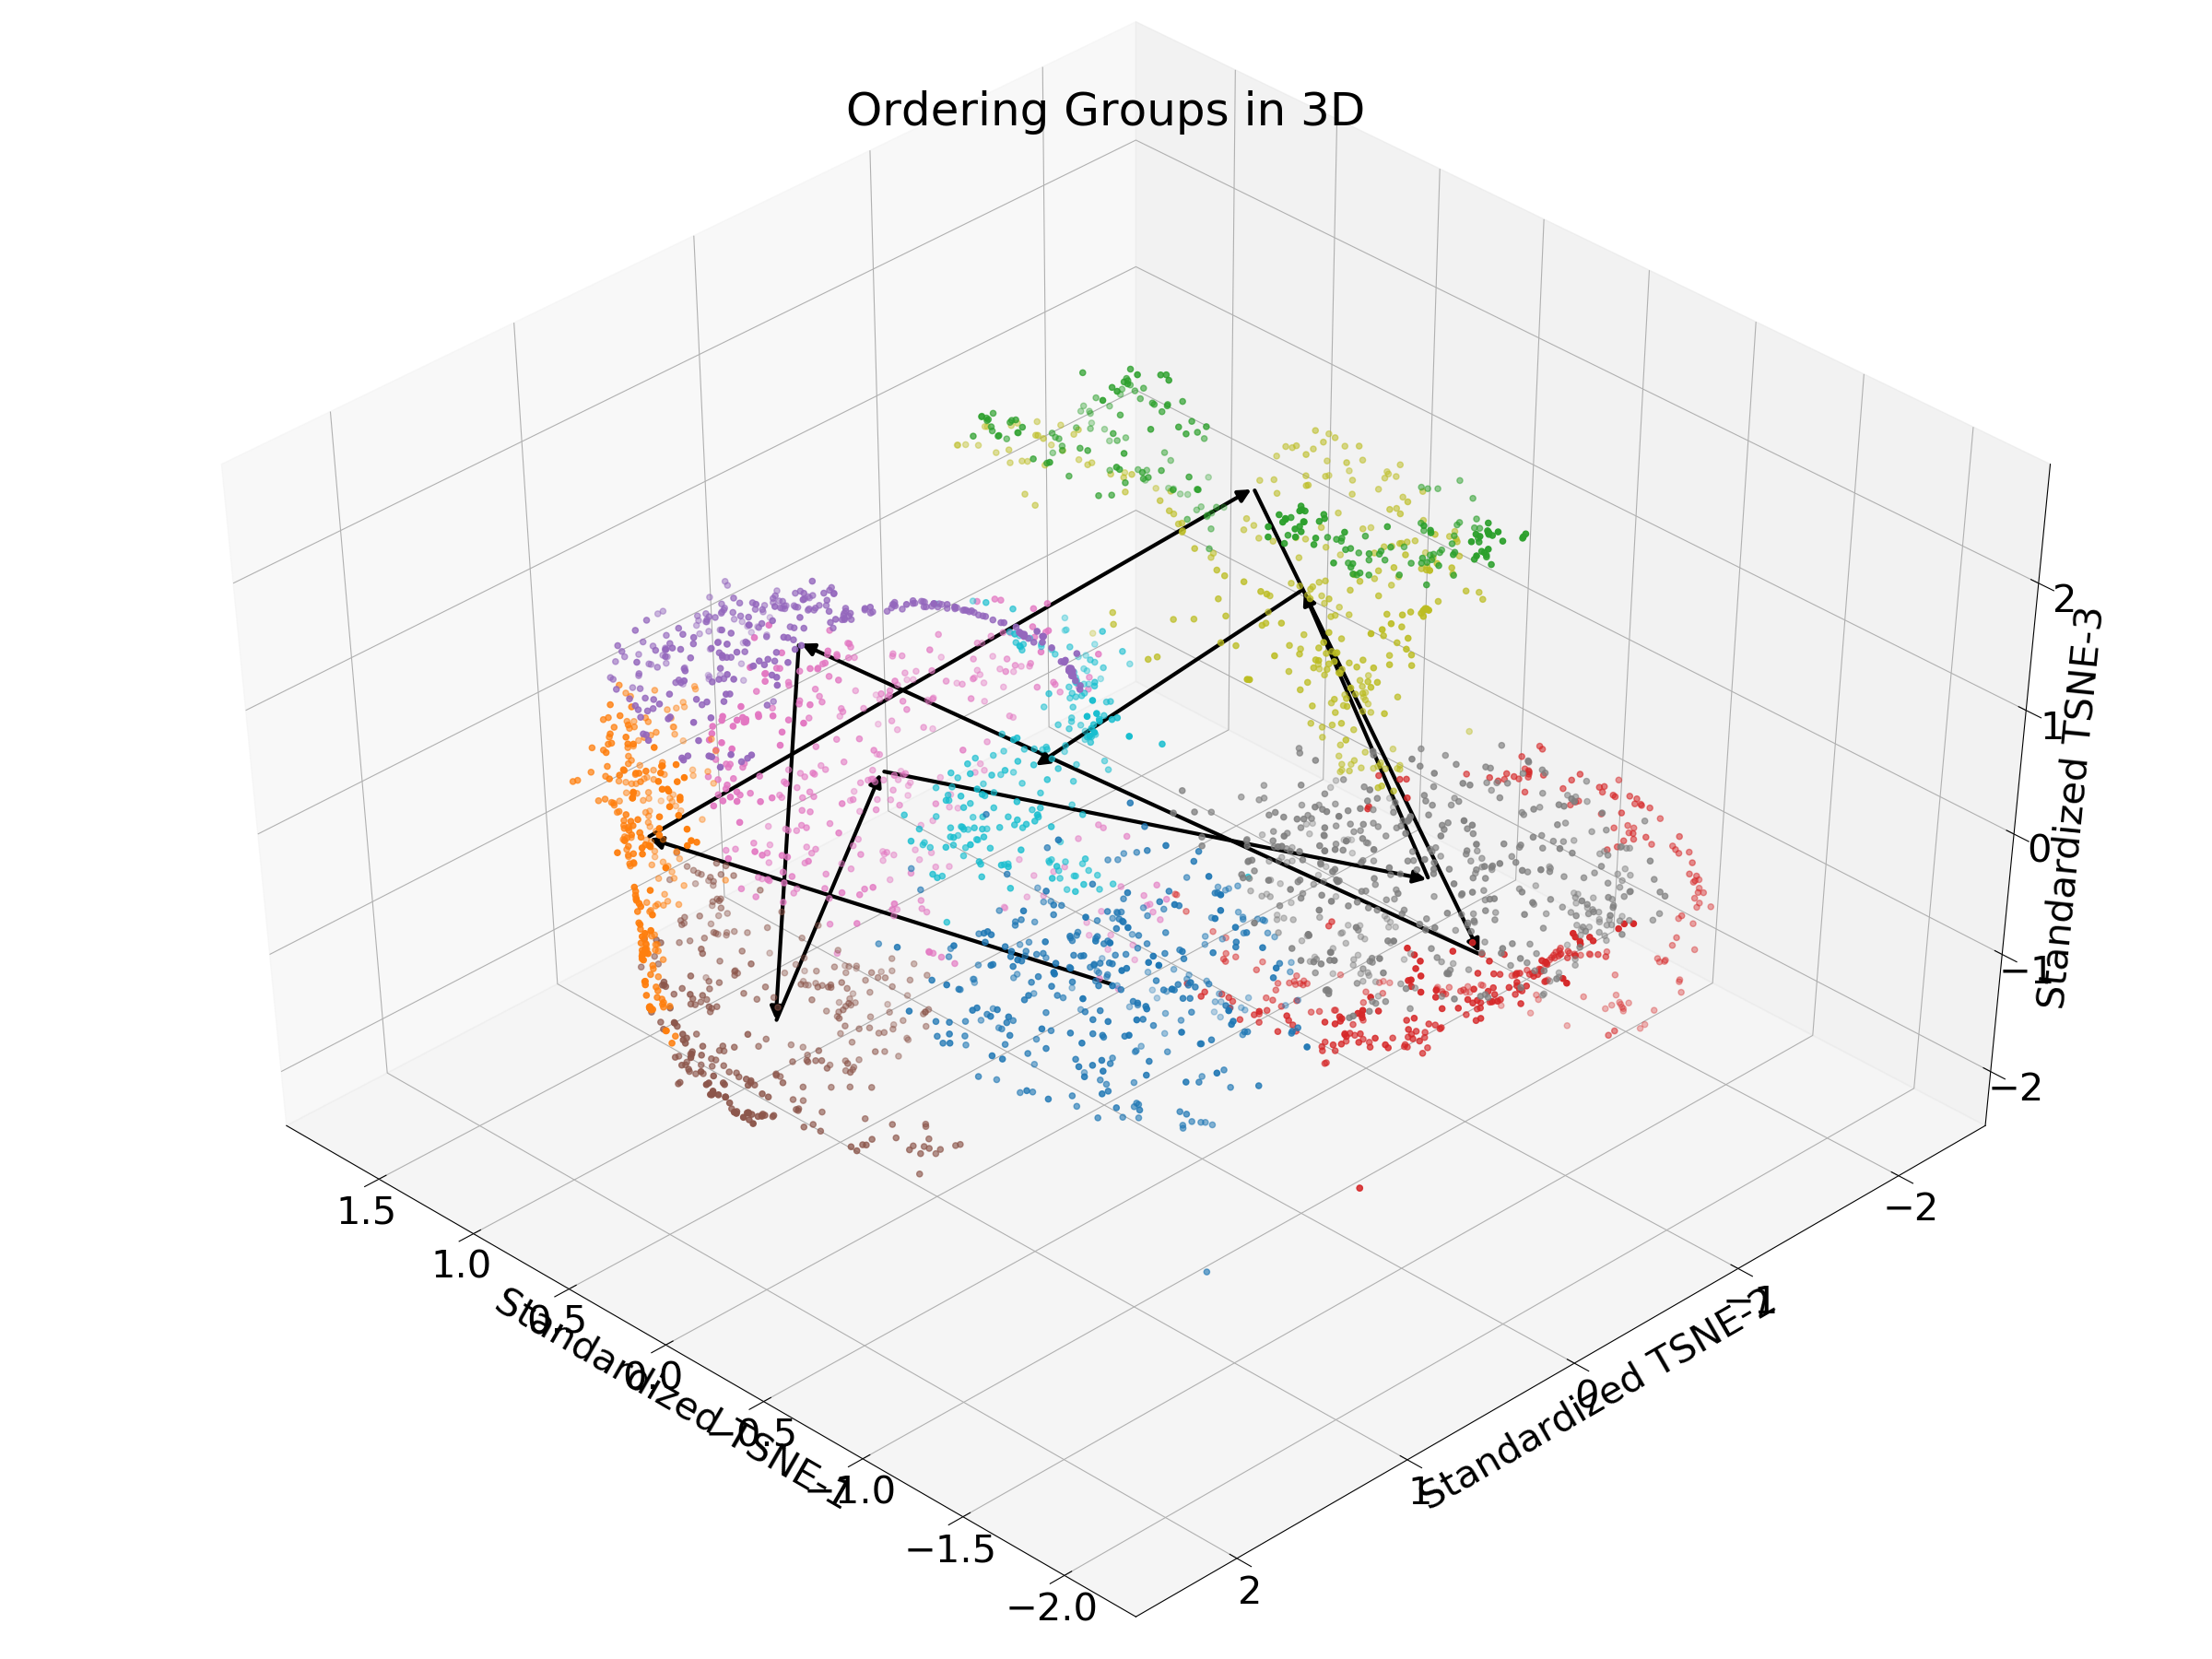
\includegraphics[height=5cm]{figures/Pseudotime/Top10/3.png}
                            &
                            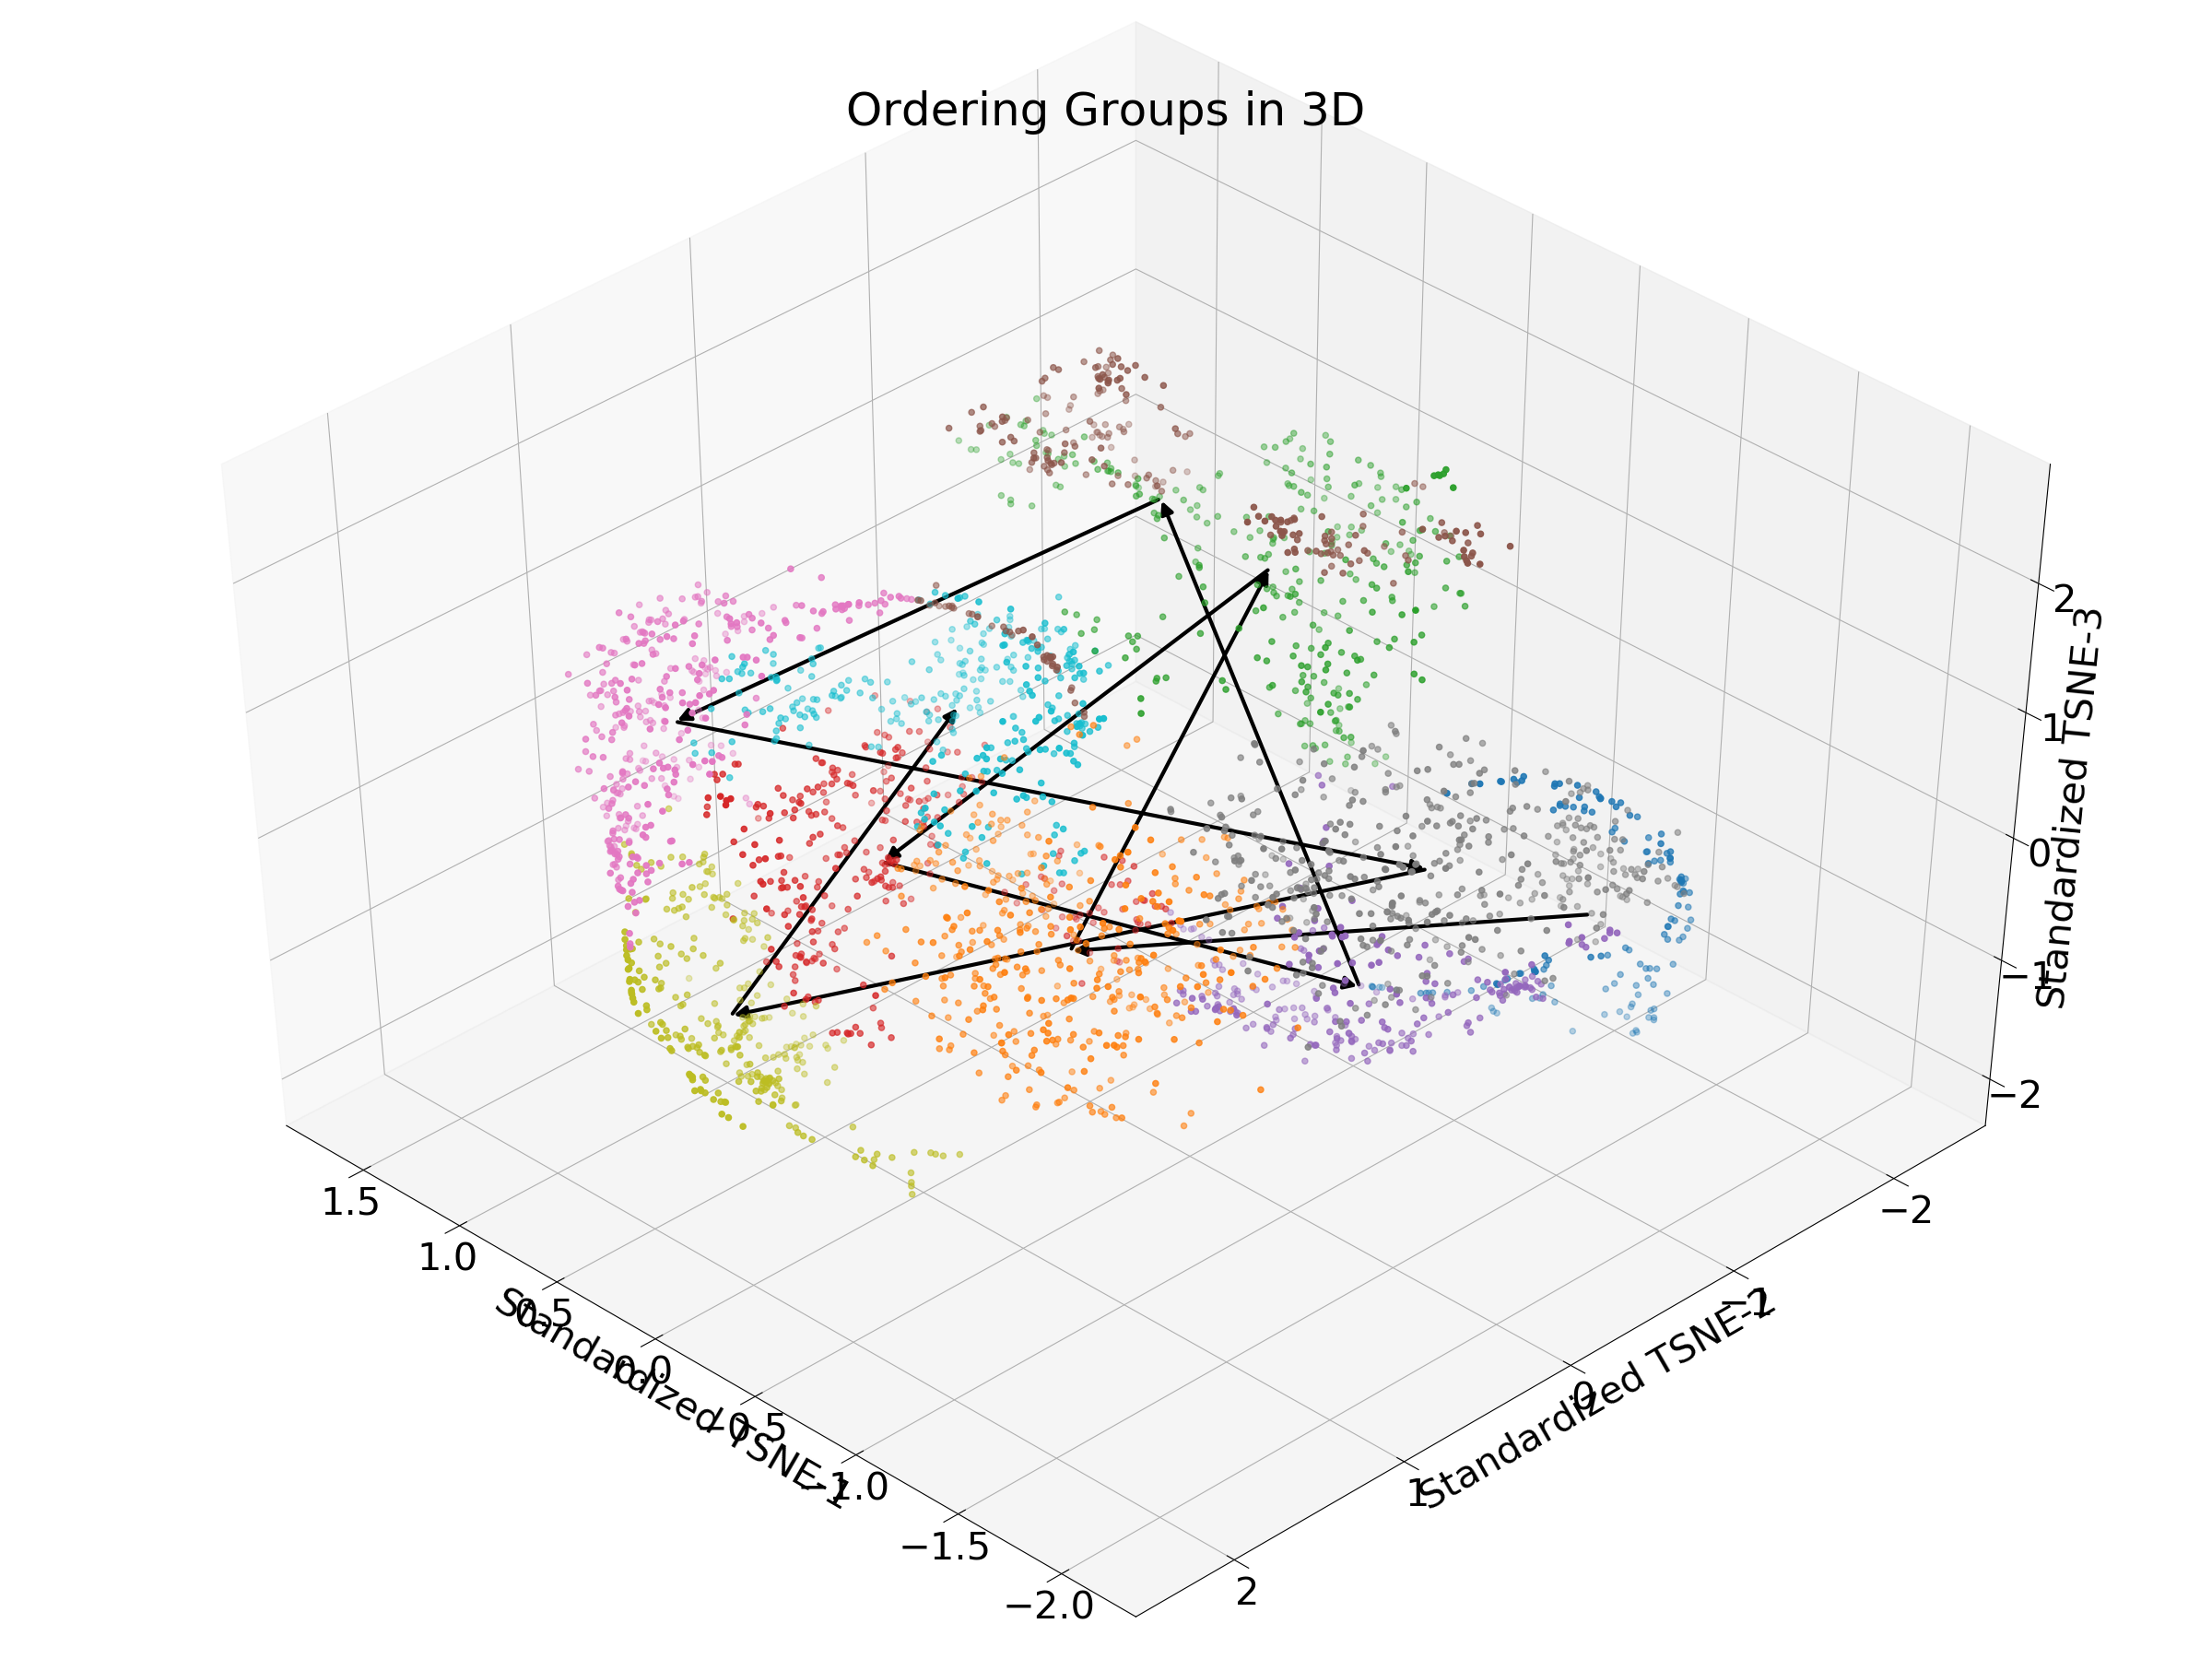
\includegraphics[height=5cm]{figures/Pseudotime/Top10/4.png}
                            \\
                            
                            \mbox{(c) NS\_SW3} & \mbox{(d) NS\_SW4} \\
                        \end{array}$
                    \end{center}
                    \caption{Pseudo-time Plot with 10 Gene which have Highest Expression}
                    \label{fig:time10gene}
                \end{figure}
    
    \section{Discussion}
        I have studied about single cell trajectory and pseudo-time analysis via this study. However, this study has some limitation points. \\
        At first, a weakness of algorithm in finding orders of cluster. According to algorithm, every gene should have only one local maximum; however, some genes, such as ID4, have more than one local maximum during spermatogenesis. \cite{ref:sperm} \\
        Second, the best combination of genes have not discovered. Some well-known marker gene have not been detected in this study. Hence, I should find the best combination upon each single cell RNA sequencing. \\
        At last, small cell number has made limitation. In the reference, they have used 62,000 cells; however, I only have 11,000 cells for RNA sequencing. Therefore, small cell number might occur some miss in RNA sequencing.
    
    \section{Acknowledgment}
        This study has been supported by Inkyung Jung Lab (\url{https://junglab.wixsite.com/home}).
    
    \addcontentsline{toc}{section}{References}
    \bibliographystyle{apalike}
    \bibliography{reference}

    
\end{document}